\documentclass{report}



\usepackage[english]{babel}
\usepackage[utf8]{inputenc}
\input{ix-utf8enc.dfu}
\usepackage{graphicx}
% \usepackage{svg}

% \usepackage[colorinlistoftodos]{todonotes}
\usepackage{float}
\usepackage{multirow}
\usepackage[table,xcdraw]{xcolor}

\usepackage{caption}  % Use for \captionof(*) command
\usepackage{subcaption}
\usepackage{pdfpages}


% \usepackage{authblk}
% 
% 
\usepackage{titlesec}

\setcounter{secnumdepth}{4}
\setcounter{tocdepth}{3}


\usepackage[Glenn]{fncychap}

% \usepackage[sorting=none]{biblatex}


\usepackage{fancyhdr}
\usepackage{extramarks}
\usepackage{amsmath}
\usepackage{amsthm}
\usepackage{amsfonts}
\usepackage{parskip}
\usepackage[version=3]{mhchem} 
\usepackage{fixltx2e}
\usepackage{refcount}
\usepackage{siunitx}
\usepackage{lastpage}
\usepackage{textcomp}
\usepackage{xfrac}
\usepackage{lmodern}
\usepackage[hidelinks]{hyperref}
\usepackage{cool}
\usepackage{cancel}
\usepackage{microtype}
\usepackage{gensymb}

% \usepackage{natbib}
\usepackage{etoolbox}
\patchcmd{\chapter}{\thispagestyle{plain}}{\thispagestyle{fancy}}{}{}


\usepackage [autostyle, english = american]{csquotes}
% \MakeOuterQuote{''}


\pdfoptionpdfminorversion=6



% \usepackage{notoccite}


%
% Basic Document Settings
%

\topmargin=-0.45in
\evensidemargin=0in
\oddsidemargin=0in
\textwidth=6.5in
\textheight=9.0in
\headsep=0.25in

\linespread{1.1}

\clubpenalty = 10000
\widowpenalty = 10000

\fancypagestyle{fancyTOC}{
    \lhead{\MakeUppercase{\rightmark}}
  \chead{}
  \rhead{}
  \lfoot{\MakeUppercase{\leftmark} }
  \cfoot{}
  \rfoot{\thepage}
  \renewcommand{\headrulewidth}{0.4pt}
  \renewcommand{\footrulewidth}{0.4pt}

%   \renewcommand{\chaptermark}[1]{%
%   \markboth{#1}{}}
}

\fancypagestyle{fancyacronym}{
    \lhead{LIST OF ACRONYMS}
  \chead{}
  \rhead{}
  \lfoot{LIST OF ACRONYMS }
  \cfoot{}
  \rfoot{\thepage}
  \renewcommand{\headrulewidth}{0.4pt}
  \renewcommand{\footrulewidth}{0.4pt}

%   \renewcommand{\chaptermark}[1]{%
%   \markboth{#1}{}}
}

\fancypagestyle{fancy2}{
% \lhead{\nouppercase{\rightmark}}
 \lhead{\rightmark}
 \chead{}
  \rhead{}
%   \lfoot{\thechapter\ \ \ \nouppercase{\leftmark} }
  \lfoot{\thechapter\ \ \ \MakeUppercase{\leftmark} }
  \cfoot{}
  \rfoot{\thepage}
  \renewcommand{\headrulewidth}{0.4pt}
  \renewcommand{\footrulewidth}{0.4pt}

%   \renewcommand{\chaptermark}[1]{%
%   \markboth{#1}{}}
}


\pagestyle{fancy}
% \lhead{\nouppercase{\rightmark}}
 \lhead{\rightmark}
 \chead{}
  \rhead{}
%   \lfoot{\thechapter\ \ \ \nouppercase{\leftmark} }
  \lfoot{\thechapter\ \ \ \MakeUppercase{\leftmark} }
  \cfoot{}
  \rfoot{\thepage}
  \renewcommand{\headrulewidth}{0.4pt}
  \renewcommand{\footrulewidth}{0.4pt}

  \renewcommand{\chaptermark}[1]{%
  \markboth{#1}{}}



\setlength\parindent{0pt}
\setlength\parskip{1.5ex}





%
% Create Problem Sections
%

% \newcommand{\enterProblemHeader}[1]{
%     \nobreak\extramarks{}{Problem \arabic{#1} continued on next 
% page\ldots}\nobreak{}
%     \nobreak\extramarks{Problem \arabic{#1} (continued)}{Problem \arabic{#1} 
% continued on next page\ldots}\nobreak{}
% }
% 
% \newcommand{\exitProblemHeader}[1]{
%     \nobreak\extramarks{Problem \arabic{#1} (continued)}{Problem \arabic{#1} 
% continued on next page\ldots}\nobreak{}
%     \stepcounter{#1}
%     \nobreak\extramarks{Problem \arabic{#1}}{}\nobreak{}
%     
% }
% 
% \setcounter{secnumdepth}{0}
% \newcounter{partCounter}
% \newcounter{homeworkProblemCounter}
% \setcounter{homeworkProblemCounter}{1}
% \nobreak\extramarks{Problem \arabic{homeworkProblemCounter}}{}\nobreak{}

%
% Homework Problem Environment
%
% This environment takes an optional argument. When given, it will adjust the
% problem counter. This is useful for when the problems given for your
% assignment aren't sequential. See the last 3 problems of this template for an
% example.
%
% \newenvironment{homeworkProblem}[1][-1]{
%     \ifnum#1>0
% 	\setcounter{homeworkProblemCounter}{#1}
%     \fi
% %     \section{Problem \arabic{homeworkProblemCounter}}
%     \setcounter{partCounter}{1}
%     \enterProblemHeader{homeworkProblemCounter}
% }{
%     \exitProblemHeader{homeworkProblemCounter}
%     \pagebreak
% 
% }

%
% Homework Details
%   - Title
%   - Due date
%   - Class
%   - Instructor
%   - Author
%
% 
% \newcommand{\hmwkTitle}{Homework\ \# 09}
% \newcommand{\hmwkDueDate}{16 April 2015}
% \newcommand{\hmwkClass}{NE 150}
% \newcommand{\hmwkClassInstructor}{Professor Max Fratoni}
% \newcommand{\hmwkAuthorName}{Andrew S Voyles}

%
% Title Page
%

\title{Our Title}

\date{Some date}

\author{\textbf{Contributing Authors:}\\ \\
James	Bevins\\
% Christopher	Brand - Naughty...\\
Christopher	Brand \\
Grant	Buster\\
Denia	Djoki\'{c}\\
Andrew	Greenop\\
Eric	Harvey\\
Tom	Hickey\\
% \'{A}nth\'{o}n\'{y}	J\'{u}\'{a}r\'{e}z\\
Anthony	Juarez\\
% Azimbek	Jumakulov - Naughty...\\
Azimbek	Jumakulov \\
James	Kendrick\\
% Nicolas	Mertz - Naughty...\\
% Diana	Othman - Naughty...\\
% Scott	Parker - Naughty...\\
% Bushra	Samimi - Naughty...\\
Nicolas	Mertz \\
Diana	Othman \\
Scott	Parker \\
Bushra	Samimi \\
Julie	Stabile\\
Andrew	Voyles\\
Xin	Wang
}



\renewcommand{\part}[1]{\textbf{\large Part 
\Alph{partCounter}}\stepcounter{partCounter}\\}

%
% Various Helper Commands
%

% Useful for algorithms
\newcommand{\alg}[1]{\textsc{\bfseries \footnotesize #1}}

% For derivatives
\newcommand{\deriv}[1]{\frac{\mathrm{d}}{\mathrm{d}x} (#1)}

% For partial derivatives
\newcommand{\simplepderiv}[2]{\frac{\partial}{\partial #1} (#2)}

% Integral dx
\newcommand{\dx}{\mathrm{d}x}

% Alias for the Solution section header
\newcommand{\solution}{\textbf{\large Solution}}

% One sentence of lorem ipsum text
\newcommand{\shortlipsum}{Lorem ipsum dolor sit amet, consectetuer adipiscing 
elit.}

% Pad zeroes for footer numbering
\newcommand\twodigits[1]{%
  \ifnum#1<10 0#1\else #1\fi
}

% Consistant figure references
\newcommand{\figref}[1]{Figure~\ref{#1}}

% Define partial derivative alias
\newcommand{\partialder}[1][2]{frac{\partial u}{\partial t} #1}

% Volume symbol
\newcommand{\volume}{\mathop{\ooalign{\hfil$V$\hfil\cr\kern0.08em--\hfil\cr}}\nolimits}

% Area symbol
\newcommand{\area}{\mathop{\ooalign{\hfil$A$\hfil\cr\kern0.08em--\hfil\cr}}\nolimits}

% Sin and Cos with auto-parentheses 
\newcommand{\sinp}[1]{\sin{\left( #1\right)}}
\newcommand{\cosp}[1]{\cos{\left( #1\right)}}
\newcommand{\expp}[1]{\exp{\left( #1\right)}}




% Make vectors use boldface
\renewcommand{\vec}[1]{\mathbf{#1}}


% Consistant matrix notation
\newcommand{\matr}[1]{\mathbf{#1}} % undergraduate algebra version
% \newcommand{\matr}[1]{#1}          % pure math version
% \newcommand{\matr}[1]{\boldsymbol{#1}}     % ISO complying version


% \newcommand{\myparagraph}[1]{\paragraph*{#1}\mbox{} \\}
\newcommand{\myparagraph}[1]{\paragraph*{#1\\}}



\makeatletter
% Make common definition of mean
\newcommand*\mean[1]{\overline{#1\raisebox{3mm}{}}}

% \def\toclevel@subsubsection{2}


\makeatother









\begin{document}

% \pagenumbering{arabic}
% 
% 
% \maketitle
% 
% 
% \tableofcontents
% 
% \thispagestyle{fancyTOC}


\pagenumbering{alph}
\begin{titlepage}
\maketitle
\thispagestyle{empty}
\end{titlepage}
\pagenumbering{arabic}

\pagestyle{fancyTOC}


\tableofcontents
% \thispagestyle{fancyTOC}
\pagestyle{fancyTOC}




\listoffigures
\thispagestyle{fancyTOC}


\listoftables
\thispagestyle{fancyTOC}

\newpage


\pagestyle{fancyacronym}

\chapter*{List of Acronyms}
\pagestyle{fancyacronym}

AAPA - American Association of Port Authorities

AQI -  al-Qaeda in Iraq

ASP - Advanced Spectroscopic Portal Monitor

CBP - U.S. Customs and Border Protection

DDA - Department of Disarmament Affairs

DHS - Department of Homeland Security

DIA - Defense Intelligence Agency

DNDO - Domestic Nuclear Detection Office

DoD - Department of Defense

DOS - Department of State

FBI - Federal Bureau of Investigation

FBIS - Foreign Broadcast Information Service

GA - General Assembly

GEOINT - Geospatial Intelligence

HUMINT - Human-Source Intelligence

IC- Intelligence Community

ICE - Immigration and Customs Enforcement

IMINT - Imagery Intelligence 

IAEA - International Atomic Energy Agency 

ISI - Islamic State of Iraq

ISIL - Islamic State of Iraq and the Levant

ISIS - Islamic State of Iraq and Syria

ISOO - Information Security Oversight Office

NASIC - National Air and Space Intelligence Center 

JTWJ - Jama'at al-Tawhid wal-Jihad 

LLNL - Lawrence Livermore National Laboratory

MASINT - Measurement and Signature Intelligence 

NSC - National Security Council  

NGA - National Geospatial-Intelligence Agency 

NRO - National Reconnaissance Office

NPT - Non-Proliferation Treaty

NSA -National Security Agency

ODNI - Office of the Director of National Intelligence

OSINT - Open-Source Intelligence

PNNL - Pacific Northwest National Lab

RDD - Radiological Dispersal Device

RPM - Radiation Portal Monitor

SC- Security Council

SIGINT - Signals Intelligence 

SNM - Special Nuclear Material

UN - United Nations

WMD - Weapons of Mass Destruction

\newpage

\pagestyle{fancy2}


\chapter{Executive Summary}

Where appropriate, expected countermeasures, such as shielding of radioactive sources, are discussed within the context of discerning a weak signal in a strong background. In circumstances where it is deemed essential for personnel to monitor the shipment of regular commerce or travel, including but not limited to commercial or private traffic by land, sea, or air, portal detectors and active interrogation is considered. Such locations are qualified for observation which are considered high risk or of strategic value in fielding a conventional response to attack from ISIL on the U.S., allies, or any sovereign territory for which instability is a matter of U.S. National Security. It is assumed that ISIL will prioritize counter-value over counterforce targets, since counter-value targeting is more disruptive and more effective in a campaign of terror.





\chapter{Introduction to ISIL}





   \shortlipsum
   

    
    
    
    \section{Background}
    
    \subsection{History}
    
    The Islamic State of Iraq and the Levant (ISIL)\footnote{ISIL is also known as Daesh, the Islamic State of Iraq and Syria (ISIS),  the Islamic State of Iraq and al-Sham, or simply the Islamic State (IS).} can be traced back to the founding of the militant Jihadist group Jama'at al-Tawhid wal-Jihad (JTWJ) by the Jordanian terrorist Abu Musab al-Zarqawi in 1999. al-Zarqawi's JTWJ gained both fame and notoriety throughout Iraq in the early 2000s for  a campaign of brutal beheadings and suicide bombings against both Sunni and Shia targets \cite{Zelin2014}. Despite initial conflicts with al-Qaeda in ideology and methodology, al-Zarqawi pledged allegiance to Osama bin Laden and al-Qaeda in 2004 to coordinate  their efforts to overthrow apostate Arab regimes, as well as the Western powers. To mark this pledge, al-Zarqawi renamed his group al-Qaeda in Iraq  (AQI) \cite{Gambill2004}. Despite this commitment, tensions and occasional armed conflicts between the two groups remained.
    
    Throughout the many conflicts in Iraq in the remainder of the 2000s, AQI underwent many changes in leadership, ideology, and name. These changes, primarily the deaths of much of its upper leadership (including al-Zarqawi), were caused by a combination of military pressure from U.S. troops, multiple disagreements  with bin Laden's al-Qaeda, and backlash from other Sunnis in Iraq \cite{Zelin2014,Kahl2008}. As a result of this, AQI was reorganized as the Islamic State of Iraq (ISI) in 2007, with Abu Bakr al-Baghdadi as it newly appointed leader \cite{Zelin2014,Shadid2010}. Under the new leadership of al-Baghdadi, ISI broke a period of regional détente with al-Qaeda (following the death of Osama bin Laden in August 2011), driving a further wedge between the two groups by al-Baghdadi's refusal to pledge allegiance to the new leader of al-Qaeda, Ayman al-Zawahiri \cite{Al-Jawlani}. In April 2013, this division resulted in  al-Baghdadi announcing that ISI would be extending its reach into Syria, and changing its name to the Islamic State of Iraq and al-Sham, or the Islamic State of Iraq and the Levant \cite{Zelin2014,Al-Hussaini2013}. In June 2014, al-Baghdadi declared ISIL a global Caliphate, with himself as its Caliph \cite{Mortada2014,TheWeek2014}. To understand the significance of this declaration, let us consider the history and role of Caliphs and Caliphates in Islam.
    
    


\subsection{Legitimacy of the Caliphate}

The origin of the Islamic concept of a Caliphate can be traced back to the foundations of Islam by Muhammad, and his organization of the Arabian peoples (who became the first Muslims) into a single theocratic society  \cite{schmidt2004great,holt1977cambridge}. This society was called a Caliphate, and was envisioned as a single state, led by a divinely-appointed leader called a Caliph, with full authority over government, religion, and military strength for all Muslims worldwide \cite{lapidus2002history}. Furthermore, as based upon the teachings of the Quran and Hadith, the Caliphate is obligated to conquer the world through Jihad, but the West in particular, creating a global Caliphate with all peoples either converted into Islam, or unbelieving subjects of the Caliphate \cite{dawood2003koran,arabi2008divine,karsh2007islamic}. Following the death of Muhammad in 632, there was a brief period of consensus over leadership, but a dispute quickly arose over who would lead the Muslims as Caliph, a schism that exists still today. Sunni Muslims believe  Abu Bakr, the father-in-law of Muhammad, was the rightful successor and Caliph, and that future Caliphs should be elected by the Muslim community. In contrast, Shia Muslims believe  Ali, the son-in-law of Muhammad, was the rightful successor and Caliph, and that future Caliphs should be direct descendants of Ali \cite{karsh2007islamic,schmidt2004great}. 

Initially, the Sunnis had a majority, with Abu Bakr assuming power as the first Caliph. Following the death of Abu Bakr in 634, two other Sunni Muslims were selected as the next two Caliphs \cite{schmidt2004great}. After decades of fighting and assassinations between these two early sects, Ali became Caliph in 656, but his reign was filled with great internal chaos. Following his death in 661, the reign passed on to his son, Hasan, ushering in centuries of expansion under the dynastic Caliphates, the Umayyad Caliphate (661–750), and Abbasid Caliphate (750–1517) \cite{schmidt2004great,oliver2009caliphate}. By 1517, the Abbasid Caliphate had its seat of power located in Cairo; when the Ottoman Empire annexed Cairo, the Ottomans usurped the office of the Caliph from that last Abbasid Caliph. This ushered in a period of even more rapid expansion under  the Ottoman Caliphate, which lasted until 1924, when Turkey abolished the Caliphate as part of secular and constitutional reform following the Treaty of Versailles of 1919 \cite{schmidt2004great,ozoglu2011caliphate}. The remainder of the Middle East was divided up into largely British and French protectorates, which remains as a point of grievance for many Muslims.

Since the abolition of the Caliphate, there have been several attempts to bring about a new Caliphate, notably the  1928 efforts of the nascent Muslim Brotherhood in Egypt \cite{Tolson2008,gabriel2008they}. However, there have been no successful attempts in the modern era, until  June 2014, when al-Baghdadi declared ISIL a global Caliphate, with himself as its Caliph and the rightful successor of the Ottoman Caliphate, citing the campaigns and expansion of ISIL as signs that ISIL is a spiritual successor of the Ottoman Caliphate \cite{Mortada2014,TheWeek2014}.  This declaration has received great criticism from not only the international community \cite{Gomes2007}, but from Muslims and other Jihadist groups as well \cite{Mandhai2014,Moore2014}. ISIL's many acts of terrorism, war crimes, and human rights violations have drawn strong criticism from the international community. From within the Muslim community, the criticism stems from the ISIL Caliphate being invalid under Islamic law, as they do not have a direct line of succession from the previous Ottoman Caliphate. In addition, many Muslims and Muslim clerics fear that the brutal and violent operations of ISIL, as well as its extremely literal and orthodox interpretation of the teachings of  the Quran and Hadith, are \enquote{rejected by most mainstream Islamists because they feel it damages their cause to establish an Islamic system through peaceful means} \cite{Mandhai2014}. Some Muslims feel that ISIL's brutal slaughter of Muslims and non-Muslims alike distorts the teachings of the Quran and Hadith and the present is not the correct time for a Muslim global Caliphate. Some believe Muslims  should currently seek a time of peace, strengthening themselves for a time of war against the West in the future \cite{schmidt2004great,Moore2014,Wood2015}.

    


    \subsection{Ideology}
    
    ISIL is an adherent to the Salafi movement of Sunni Islam \cite{Bradley2015}, itself a very orthodox school of thought among Muslim theology.  As such, it promotes a reform of Islam back to its roots with Muhammad, and an extremely literal interpretation of the Quran and Hadith \cite{Hassan2015}. Many modern Jihadist groups are devout adherents to Salafi Islam, which requires that all true believers live the tenets of the Quran to the letter. Salafists  advocate Jihad and the conquest of all peoples (specifically the West) by forcible conversion, execution, or subjugation through conquest, driving towards a global Caliphate. ISIL shares these beliefs with other modern Islamic Jihadist groups, including the Muslim Brotherhood and al-Qaeda, due to its support of religious violence and terrorism \cite{schmidt2004great,gabriel2008they,Hassan2015,Moussalli2009}.
    
    One significant difference between ISIL and other mainstream Sunni Muslims is that ISIL violently condemns all Muslims who disagree with its interpretations as infidels and apostates, promoting  sectarian violence for deviating from the \enquote{pure Islam} that ISIL follows. They also advocate this same violence against journalists, civilians, relief workers, and any other individuals or groups whom ISIL believes are supporting any infidel \cite{Wood2015,Hassan2015,AustralianNationalSecurityAttorney-GeneralsDepartment2014}. Many of the atrocities that have so shocked the world - beheadings, burnings, forced marriages - result from this commitment of ISIL to live the tenets of the Quran to the letter. It is these extreme levels of  violence (sectarian and otherwise) that has earned ISIL condemnation from mainstream Sunni and Shia clerics, as ISIL's public show of fundamentalist Islam gives Islam a violent appearance in the eyes of the global community \cite{Mandhai2014}.
    
    In line with their  orthodox and literal interpretation of Islamic teachings, ISIL  has a strict literal interpretation of Islamic  end-times theology. ISIL teaches that the world is currently in the beginning of the end times, and that their actions are intended to hasten the arrival of Imam Mahdi, a Muslim messianic figure prophesied by Muhammad in the Hadith, whose rule will precede the end of all times \cite{arabi2008divine,Wood2015}. ISIL believes that when the Mahdi arrives, the global Caliphate (with ISIL at its head)  will \enquote{await the army of \enquote{Rome,} whose defeat at Dabiq, Syria, will initiate the countdown to the apocalypse} \cite{Wood2015}. However, from the declarations of ISIL, it is unclear what \enquote{Rome} actually represents - America, the West, Turkey (whose abolishment of the Ottoman Caliphate is seen as an act of supreme treachery against all Muslims, and earns them a particular vehemence from ISIL), any \enquote{apostate} group from ISIL's standpoint, or some other institution which represents an archetype of anti-Caliphate authority to ISIL \cite{Mortada2014,Wood2015}. 
    
    
    


\subsection{Land}

\subsubsection{????? Missing ?????}

\subsection{People}

\subsubsection{????? Missing ?????}


\subsection{State functions/income}

\subsubsection{????? Missing ?????}


\subsection{How does this relate to their potential nuclear interests?}
\subsubsection{????? Missing ?????}
\subsubsection{????Move in info from mat / signatures group????}

we can pull from what the State Department is already doing on this

    
    


\section{Goals}

\subsection{????????  Needs expansion  and references   ????????????}

Since ISIL began to seize power and land in Iraq and Syria, many of studied what exactly drives the organization. Perhaps the most complete discussion of the group's motivation comes from Graeme Woods' article \enquote{What ISIL Really Wants,} which appeared in the March 2015 issue of The Atlantic \cite{Wood2015}. In assessing ISIL and its goals, it is first necessary to recognize its differences with other militant Islamic terrorist organizations. 



The strict brand of Salafism which ISIL espouses has also led to another important distinction between ISIL and other terrorist organizations: the establishment of a Caliphate, with Abu Bakr al-Baghdadi as Caliph. A Caliphate is a homeland for Muslims, and ISIL believes that its establishment is necessary for it to truly follow the tenets of Islam. While other terrorist organizations were content to live amongst the people in various countries, ISIL has seized territory and established a government. In their orthodox and literal interpretation of Islam, the division of the Middle East into its current countries was driven by Western countries, and is therefore fundamentally illegitimate and cannot be tolerated. 

The taking and protection of territory by ISIL is one of its core goals. Under the tenets of Salafism, a Caliphate cannot exist without land, and so maintaining a geographic foothold is fundamental to the existence of ISIL. Without it, their caliphate will cease to exist. 

Much discussion has surrounded the flow of foreign fighters into ISIL controlled territory. Again, this is rooted in the groups' religious beliefs. According to Salafism, once a caliphate is established, all true believers must move to it, unless completely unable to do so. 

ISIL poses a more direct threat to its neighbors than to the U.S. homeland. While many foreigners with Western passports have pledged allegiance to ISIL, they often do so with no intent to return, as illustrated by the common burning of passports once individuals reach ISIL territory. Additionally, ISIL must continue to expand, taking territory from “illegitimate” governments, in order to maintain its own legitimacy as a Caliphate. 


\subsection{What makes this a different problem than traditional non-proliferation efforts?}

\subsubsection{????? Missing ?????}

Missing


\subsection{Framework for how this report is formed}

\subsubsection{????? Missing ?????}

Missing


\subsection{Their potential targets (“declaratory policies”)}

\subsubsection{????? Missing ?????}

Missing

\section{Global Relationships} \label{sec:global_rels}





In assessing how ISIL may acquire a nuclear weapon, it is necessary to consider potentially helpful alliances and allies, as well as their enemies.  As with most things related to ISIL and the Middle East, this is not necessarily as straightforward as one would assume.  While some relationships are fixed points of reference, most are dynamic and characterized by opportunism, both on the part of ISIL and the organization or state who seeks to gain some benefit from supporting or opposing them.  The following discussion is not intended to be all encompassing but instead will focus on key players and how they may help or hinder ISIL's nuclear ambitions.  

At first glance, the strategic landscape does not look favorable to ISIL as depicted in \autoref{fig:ISILRelationships} below.  While somewhat dated, it serves a decent representation of some of the key groups and states that are in direct conflict and collaboration with ISIL.  ISIL's key relationships can be broadly grouped into three categories:  countries and groups at war with ISIL, former or potential future allies, and groups that support ISIL.  

 \begin{figure}[h]
 \centering
 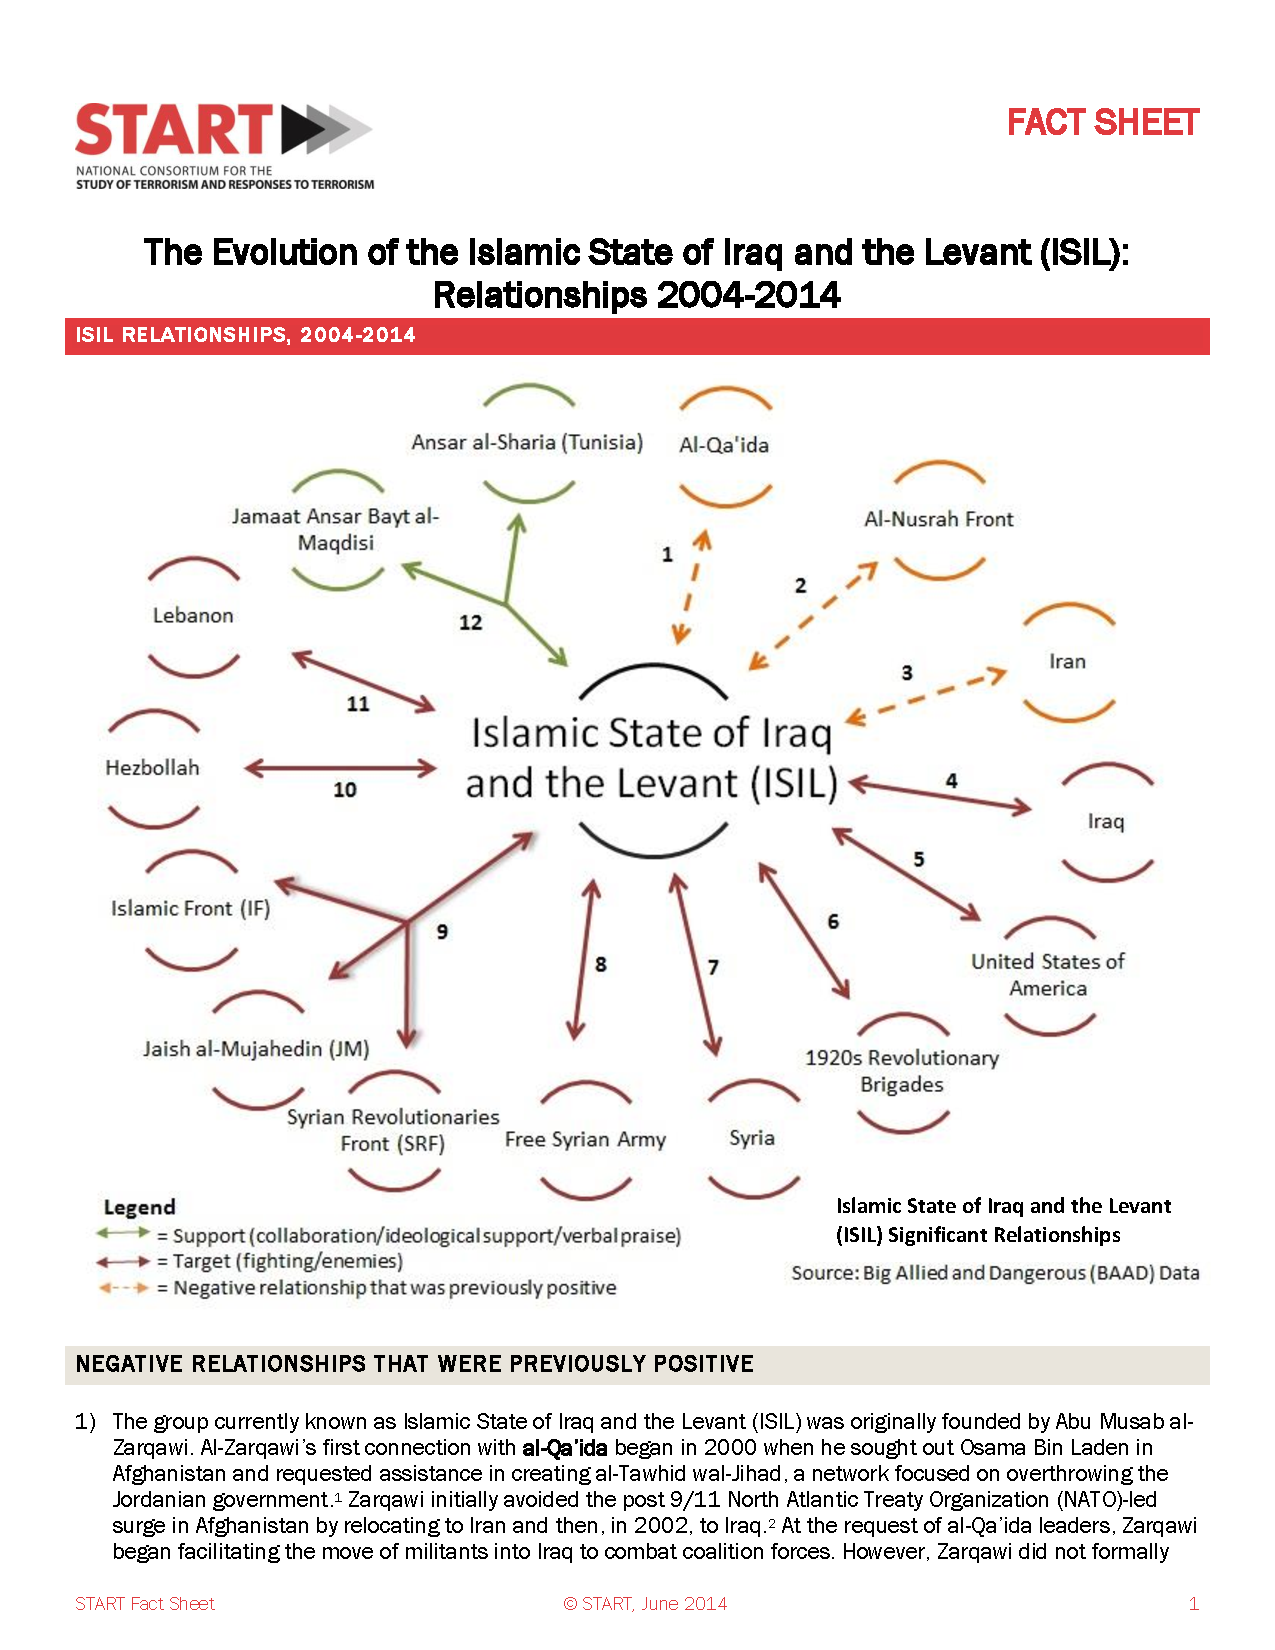
\includegraphics[trim = 0cm 5.9cm 0cm 5.35cm, clip,scale=0.6]{./figures/ISILRelationships.pdf}
   \caption{ISIL relationships as of mid-2014.  Note the figure uses the alternative name of ISIL that was preferred by the Obama administration for ISIL \cite{NationalConsortiumfortheStudyofTerrorismandResponsestoTerrorism2014}}
     \label{fig:ISILRelationships}
\end{figure}



% \subsection{Countries and Groups at War with ISIL}

ISIL has many enemies, indeed many more than are graphically depicted in \autoref{fig:ISILRelationships}.  As of January 2015, the anti-ISIL coalition led by the U.S. included 62 nations and groups including the U.S., Canada, Iraq, Jordan, Bahrain, Saudi Arabia, UAE, France, Germany, United Kingdom, Australia, Belgium, Denmark, Italy, Czech Republic, Albania, Netherlands, Estonia, Hungary, Turkey, and Lebanon, all of whom have carried out or supported military operations against ISIL \cite{Wordsworth2015}.  Additionally, although not allied with the U.S. coalition, Syria, Iran, and various Kurdish, Shia, and Sunni militias in Syria and Iraq have opposed ISIL \cite{Mooney2014}.  Despite this broad coalition, there are many unlikely allies in the list which present potential seams for ISIL exploitation  through propaganda or military action.  For example, strikes against ISIL in Syria benefit the Assad regime while U.S. trained rebels could turn on and attack the Assad regime \cite{Shinkman2015}.  Officially, the U.S. supports the removal of the Assad regime albeit without direct military intervention on part of the U.S. \cite{Shinkman2015}.  Similarly, U.S. air strikes and intelligence have supported Iran and Iraqi Sunni and Shia militias (including several that once fought U.S. forces) in their campaigns against ISIL \cite{Chulov2014}.  While these uneasy alliances have placed pressure on ISIL, it is unclear if they can be sustained over the timeframe that would be necessary to defeat ISIL and prevent their acquisition of a nuclear weapon. Sustaining these alliances would be especially difficult if ISIL were to turn its formidable propaganda machine to breaking some of these fragile links.


Additionally, there are longstanding mistrust, perceptions, and illicit alliances that could cause large fissures  without the help of ISIL.  While the Iraqi government is cooperating with the U.S. in battling ISIL, some clerics and government officials have publicly claimed the CIA was responsible for the rise of ISIL \cite{Kirkpatrick2014}.  Whether this is true is largely irrelevant if the mere perception affects the extent of U.S. - Iraqi cooperation against ISIL, especially if the need would arise to place U.S. troops in combat.  Other reports have the Turkey military providing safe travel and weapons for ISIL fighters attacking Kurdish forces, which have been a thorn in the side of Turkey \cite{Guiton2014}.  Finally, it appears that wealthy Saudis, who have a history of funding terrorist organizations, are continuing to provide ISIL with funding \cite{Windrem2014}. While this funding and free travel is not a large contributor to ISIL's overall success, it represents larger issues faced in isolating ISIL from the international community and shows a willingness of certain groups to deal with ISIL if they see personal benefit despite the international condemnation.  Currently, it is just guns, cash, and ammunition, but as time wears on does someone sell nuclear components or technology to ISIL in an attempt to accomplish some goal?  It may sound unfathomable, but perhaps no more irrational that the U.S. arming militias and rebels in Syria, despite the fact that the current issues facing the Middle East with regards to terrorism and ISIL can be traced to the U.S. arming and training of Afghani rebels in the 1980s. 

% \subsection{Groups  supporting ISIL}


Although the increasing coalition arrayed against ISIL is a promising curb to their  nuclear ambitions, the growth of ISIL's alliances is not.  Currently, ISIL has 32 affiliates throughout the world of varying size and level of support \cite{IntelCenter2015}.  A map of the countries where those organizations operate is shown in \autoref{fig:affmap}.  Two important countries in the region with respect to nuclear issues stand out.  First, Iran is currently opposed to ISIL, has no organizations pledging support to ISIL, and is funneling support for Iraq and Hezbollah to combat the spread of ISIL.  However, Iran is no stranger to supporting terrorist organizations that it believes can advance its interests, and it has previously shown tendencies to cross sectarian lines for even tenuous, direct, or indirect gain to Iran \cite{pollack2014unthinkable}.  Pakistan, on the other hand, has had no shortage of declared support, and many believe that trend is to continue \cite{IntelCenter2015,Walsh2014}.  While Pakistan is firm in statements about the control of its nuclear weapons, their program has had a history of proliferation and is widely considered to have ongoing commitments to sell nuclear weapons should the need arise \cite{Langewiesche2005,Henderson2015,Smith2011}.  Due to the consequences, the low probability event of Pakistan or Iran aiding ISIL's nuclear ambitions poses unique challenges in the goal of preventing ISIL from obtaining nuclear weapons. 


\begin{figure}[h]
 \centering
 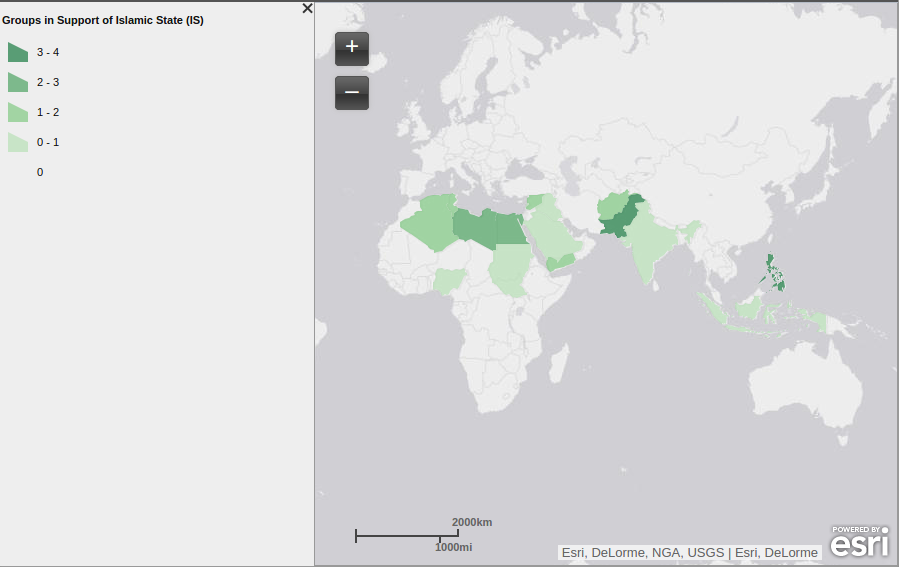
\includegraphics[scale=0.4]{./figures/affmap.png}
   \caption{Map of countries with ISIL affiliates \cite{IntelCenter2015}. }
     \label{fig:affmap}
\end{figure}



When considering ISIL's nuclear ambitions, one country not currently entangled in the ISIL conflict must be considered: North Korea.  In the past, North Korea has shown a willingness to export nuclear technology \cite{Wit2013}.  Some have argued the test of an uranium device in 2013 was an advertisement to the world that it could produce excess nuclear weapons that may be available for sale \cite{Allison2013}.  Currently, there is no known relationship between ISIL and North Korea.  However, given the unpredictability of the North Korean regime, coupled with the fact that there are operatives throughout ISIL controlled territory that would have North Korean contacts due to the prior Syrian - North Korean nuclear collaborations, any attempt to stop ISIL from obtaining a nuclear weapon needs to account for this potential pathway.   


Finally, it is important to consider the non-organizationally aligned support that ISIL receives in the form of foreign fighters.  The flow of these foreign fighters has dwarfed the influx associated with previous calls to Jihad, such as Afghanistan in the 1980s \cite{Barrett2014}.  These fighters come from all over the world as shown in \autoref{fig:enablers}, and they bring a diverse background and skill set with them.  Although no comprehensive list has been established in the open literature about the skills brought to ISIL via foreign fighters, it is likely that some of the foreign fighters possess skills necessarily to develop, fabricate, and assemble components of a nuclear weapon. 

\begin{figure}[h]
 \centering
 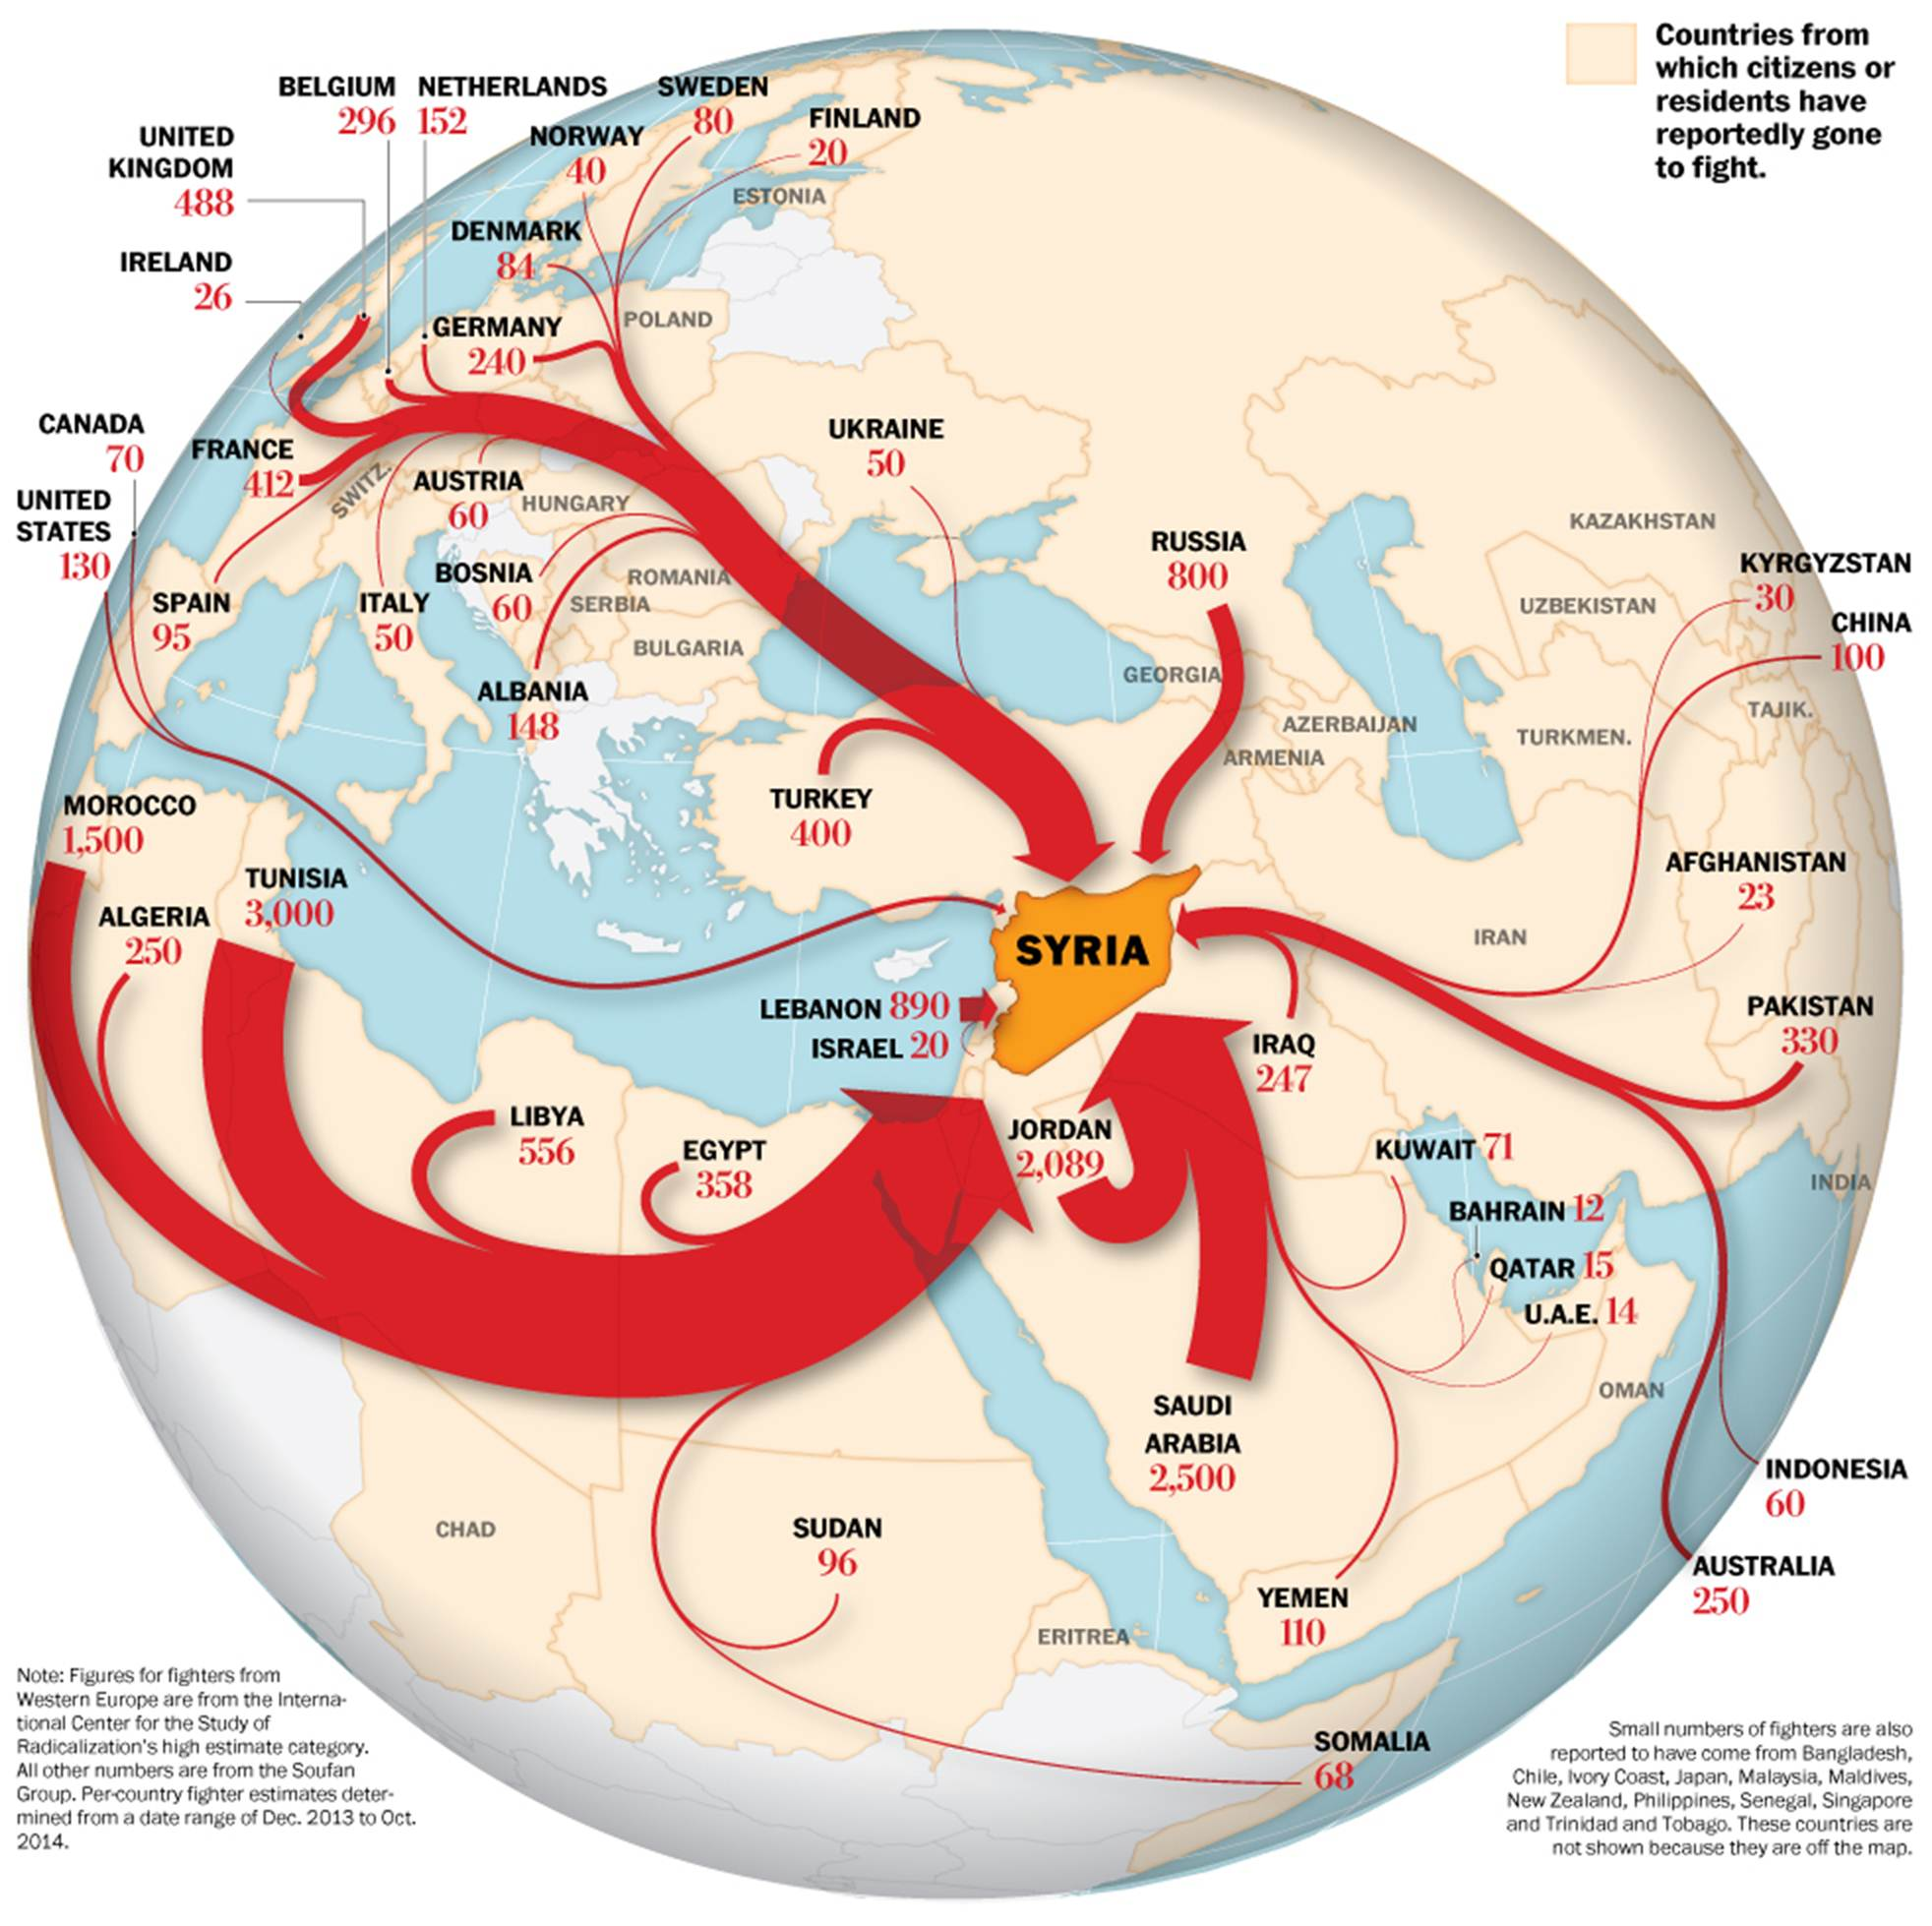
\includegraphics[scale=0.6]{./figures/enablers.jpg}
   \caption{Flow of foreign fighters into Syria \cite{Thorp2014}. }
     \label{fig:enablers}
\end{figure}







\chapter{Problem Definition}

\section{The Threat of an ISIL  Nuclear Weapon}

The threat of  nuclear weapon states is not a novel thought. Being the first and only nation to use a nuclear weapon against an enemy, the United States has feared a nuclear threat ever since weaponized nuclear technology became possible. Shortly after, the Soviet Union acquired nuclear weapons, marking the onset of the nuclear standoff during the Cold War.   Fortunately, through deterrence based on game theory against a rational adversary, not a single shot was fired between the U.S. and the USSR for approximately 44 years, until the conflict was alleviated. Since then, the nuclear threat has spread to many nations, including, most recently, Iran. 

The Iranian nuclear program has been called \enquote{the most vexing foreign policy challenge confronting the Obama administration}, and it is quite possibly the most difficult foreign policy challenge that the world has seen in many years \cite{Edelman2011}. Others have argued that Iran, as a large nation with much to lose, will develop the caution and restraint that is typically incurred by nuclear weapons development. This chain of events: weapons development, fear on a global scale, effective deterrence, and eventual restraint, has always been the crux of global nuclear weapons security. 

The world has not yet seen a nuclear capable entity    that is not sufficiently deterred by the threat of their own destruction. This is what makes ISIL a case of unique consideration. ISIL cannot be bundled into either the category of nations with inherent fear of self-destruction or the category of non-state actors with insufficient resources. They have continued to prove themselves as an organized and intelligent group that can continue to surprise the world with their capabilities. Their radically extremist ideology, vast independent wealth, powerful military, and pure ferocity set them apart from the organizations with whom the U.S. has historically dealt  \cite{bach2015isis}. 

The probability of ISIL acquiring nuclear weapons technologies and weapons is very low, so low, in fact, that this threat has been played down, with some dismissing the idea of an indigenous ISIL nuclear enrichment program as \enquote{impossible} \cite{AlexanderSmith2014,Cirincione2014}. The probability of ISIL obtaining a nuclear weapon may be incredibly small. However, risk is defined by both the probability of an occurrence as well as its potential consequences, which could be unfathomable \cite{ONeill1997}. Further, evidence  has  been reported  of ISIL  moving to obtain special nuclear material \cite{AlexanderSmith2014}. When it comes to nuclear weapons, the world cannot afford to be  surprised by ISIL. 

These low-probability, high-consequence events and any potential preventative policies are incredibly important to thoroughly analyze. For this reason, this report will focus on policies that could be implemented to prevent ISIL from gaining access to nuclear weapons technology and materials. Bernard Brodie said it best in Wizards of Armageddon: \enquote{nuclear war is unthinkable but not impossible, and therefore we must think about it} \cite{kaplan1991wizards}.





\section{What this report will focus on}

This  report will evaluate and discuss the ability of  ISIL to engage in nuclear terrorism, so as to inform a policy statement to be enforced by the U.S.. This report considers the capability and resources of other sovereign powers and terrorist organizations when those may benefit ISIL. This policy statement details an organized response to any step ISIL may make towards the deployment of a device containing special nuclear material (SNM). It stops short of a larger policy directed towards  the Administration's goal to degrade and ultimately destroy ISIL. 

The scope of this  report is limited to the materials, signatures, and means of detection for those signatures, in all phases during the development and delivery of a nuclear device. 

This  report is directed towards the immediate response to development of the nuclear capabilities of ISIL, and does not consider the consequences which might result if ISIL were to evolve into a permanent state. This  time scale greatly reduces the possibility that ISIL possesses the infrastructure necessary to produce SNM or to assemble such material into a functioning warhead, unless they capture territory containing existing infrastructure. Due to the extreme sophistication in the triggering device, the development of fusion weapons is very unlikely in the time window considered. Rather, emphasis is placed on diverting existing SNM from existing global stockpiles.

It must be considered that ISIL may orchestrate the delivery and detonation of a fission weapon or RDD without any of the material or components passing through territory which is directly controlled by ISIL. In this scenario, the search for SNM is a global concern, and the problem of detection and interception of such weapons or the orders to carry out such attacks is one which the international community must work together to address. 



\section{Limitations and assumptions of this report (group 1)}

\subsection{?????? Julie working on this section ?????}



This policy recommendation is oriented primarily towards responding and preventing ISIL nuclear capabilities. The scope encompasses strategic communication within the intelligence community as well as among the U.S and potential countries and international entities and military capability. In the interest of time, this recommendation will not consider collaboration on information gathering or post-detonation. The following policy initiative will focus on developing an integrated intelligence strategy. 

\section{Scoping and problem - kind of summary and set framework for rest of report}

This report was completed as a part of a graduate level Nuclear Security Policy course at the Goldman School of Public Policy and the Nuclear Engineering Department at the University of California, Berkeley. The class of approximately 20, including policy students and nuclear engineering students, was tasked with developing a policy recommendation for preventing ISIL from obtaining any nuclear capabilities.

As this is only a semester long project, there were great restraints on time and therefore scope. This report focuses solely on the paths to ISIL obtaining a nuclear capability. Of course, the fundamental way to preventing this would be to defeat ISIL in its entirety. However, given that the overall destruction of ISIL is a larger administration goal and is therefore being addressed by many other groups, our report focuses solely on nuclear capabilities. We also limited our scope by assuming that this policy applies only to the immediate future, and that if ISIL were to last for a longer time frame, more traditional state non-proliferation activities could take place.




\chapter{Nuclear Weapons Primer}

A glossary of much of the nuclear-related terminology used in this paper may be found summarized in  \autoref{app:glossary}.

\section{Basic Nuclear Physics \& Definitions}

\subsection{??????   Assign to someone  ????????}

\subsection{Fission}

\subsection{???????  Needs content proofing   ????????}

\subsection{???????   Need discussion of criticality  ??????}

A fission device operates on the principle that fissile materials (list of materials) will undergo fission when stuck by neutrons of sufficient kinetic energy. A nuclide which undergoes fission will release between 100-200 MeV in addition to 2-3 neutrons, which may be utilized to cause subsequent fissions in other fissile nuclei \cite{krane1987introductory}. The minimum amount of fissile material needed in order to sustain a chain reaction is known as the critical mass, which depends on the type, density, and shape of material used. A tamper, which is a high Z material which acts as a neutron reflector, is typically used in order to reduce the critical mass. 












\subsection{Critical Mass}

The minimum amount of special nuclear material needed to produce a fission weapon is called the critical mass. This value can depend on many different features including isotope, geometry of the material, micro-structure of the material, and device design. Given the many variables in play it would be infeasible to include the critical mass of every possible weapons configuration here. However, to give a general idea, \autoref{tab:critical_mass} presents the critical mass of two different designs for several types of weapons. Additionally the yields of fission devices can vary based on many factors including, type of material, device design, amount, efficiency, and many other factors. Yields are typically on the order of kilotons \cite{Moody2014}. 


\begin{table}[h]
\centering
\begin{tabular}{|l|c|c|}
\hline
\multicolumn{1}{|c|}{Material}                                              & Critical Mass, Bare Sphere (kg) & Fully Tampered Sphere (kg) \\ \hline
\ce{^{235}U}                                                                       & 52                              & 17                    \\ \hline
\ce{^{239}Pu} (alpha phase)                                                        & 10                              & 4                     \\ \hline
\ce{^{239}Pu} (delta phase)                                                        & 16                              & 6                     \\ \hline
\begin{tabular}[c]{@{}l@{}}Reactor Grade Pu \\(60\% enriched in \ce{^{239}Pu})\end{tabular} & 13                              & -                     \\ \hline
\ce{^{233}U}                                                                      & 15                              & 6                     \\ \hline
\end{tabular}
\caption{Critical Masses of a Bare and Fully Tampered Sphere for Various Special Nuclear Materials \cite{Moody2014} }
\label{tab:critical_mass}
\end{table}





\section{Fuel Cycle}



\subsection{??????  This makes some nods towards policy, and how to use the fuel cycle in our policy, but not much  ?????????}


\subsection{Uranium}

Regardless of whether nuclear material is destined to be used in a nuclear reactor for power generation or in a nuclear weapon, much of the fuel cycle is the same. Both processes start with the mining of uranium from nature, followed by chemical purification and enrichment \cite{Moody2014}.

The most important step in the process, from a proliferation standpoint, involves enriching the uranium in \ce{^{235}U}. Natural uranium is typically 0.72\% \ce{^{235}U} \cite{Benedict1981}.  If uranium is destined for a power plant, it is typically enriched to  3-5\% \ce{^{235}U}. For use in a nuclear weapon, the uranium must be enriched to greater than approximately 90\% \ce{^{235}U} \cite{Moody2014}. 

Most enrichment is done using gas centrifuges; however, this requires significant infrastructure that is almost definitely beyond the capabilities of ISIL \cite{Benedict1981}.  Furthermore, even if ISIL were able to gain control over an enrichment facility, the length of time it would take them to enrich enough uranium for a weapon would allow other countries to intervene militarily. For example, if ISIL were to gain control of Iran's Natanz facility, it would take them approximately two (using 3.5\% enriched feedstock) to six months (using natural uranium feedstock) to enrich the uranium necessary for a weapon \cite{WisconsinProjectonNuclearArmsControl2015,Heinonen2015}. Therefore, the most significant step  in stopping ISIL from enriching uranium for a weapon is simply identifying enrichment facilities, which are difficult to hide, within or close to its territory. 

While ISIL could theoretically use laser separation to enrich uranium, which is significantly more difficult to detect, this is very unlikely. Currently, there is only one prototype process under investigation, located in Australia, making it unlikely that ISIL would use this method to enrich uranium \cite{Moody2014}. 

It is also possible that ISIL could attempt to use electromagnetic isotope separation (EMIS) to produce weapons usable material like the U.S. during World War II and Iraq before the First Gulf War. However, this seems incredulity unlikely. EMIS requires the use of machines called calutrons which are very expensive and very inefficient. For example, even with hundreds of calutrons functioning together, it still took the U.S. approximately one year to produce the uranium for the Hiroshima bomb \cite{Moody2014}. Thus, given the extreme inefficiency and lengthy enrichment time frame, it seems unlikely that ISIL would be able to construct and enrich uranium without the U.S. becoming aware and taking military action.

While gaseous diffusion is still used on a commercial scale, it does not pose much of a proliferation threat. It is an incredibly energy intensive process, requiring 50 times the power per separative unit required by the use of centrifuges \cite{WorldNuclearAssociation2015b}. If ISIL were to try and enrich uranium through gaseous diffusion, it would not be difficult for U.S. surveillance to find and destroy such a plant before they acquire enough highly enriched uranium.

One final way ISIL could attempt to enrich uranium is through chemical exchange. However, while this method has been developed in both France and Japan, it has never actually been used \cite{Africa2012}. Furthermore, this technique is not yet competitive with the other techniques discussed above, making it an unlikely choice \cite{Moody2014}. 

\subsection{Plutonium} 

While uranium appears in nature, significant quantities of plutonium are only available through irradiation in a nuclear reactor \cite{Benedict1981}. It is formed when \ce{^{238}U} undergoes the process known as neutron capture \cite{Benedict1981}. \ce{^{239}Pu}, which can be used in nuclear weapons, is produced following a double beta decay of \ce{^{238}U} \cite{Duderstadt1976}. Heavy water reactors have a higher percentage of \ce{^{238}U}, thus forming \ce{^{239}Pu} at a faster rate, and are preferred to light water reactors to produce plutonium \cite{Moody2014}. While ISIL could theoretically gain control of a commercial nuclear reactor for plutonium production, it is deemed incredibly unlikely. The only commercial nuclear reactors currently near their territory are located in Iran \cite{WorldNuclearAssociation2015}. While countries like Saudi Arabia, Egypt, Turkey, and the UAE are all moving towards nuclear power, it will be many years before any of those countries have commercial plants \cite{WorldNuclearAssociation2015}. While there are not many commercial reactors that ISIL could easily use to produce plutonium, there are many research reactors scattered throughout the Middle East \cite{WorldNuclearAssociation2015a}. However, ISIL would need to make very significant territory gains for any of the closest research reactors to be in danger \cite{BBC2015}. Thus, it seems unlikely that ISIL would be able to gain control of a nuclear reactor for plutonium production. Additionally, any captured reactor fuel would require reprocessing to separate out the plutonium. The time required would be significant enough to allow for a response.  

It should be noted that Syria may have had a reactor for the production of plutonium in the past. However, that site was bombed and destroyed by an Israeli airstrike in 2007 \cite{WorldNuclearAssociation2015a}. It is not impossible that ISIL could obtain the plans for that design. Nevertheless, construction on a nuclear power plant typically takes at least 4 years, and nuclear reactors are incredibly difficult to hide \cite{WorldNuclearAssociation2015a,NuclearEnergyInstitute2015}. Therefore, there is a very low probability that ISIL could covertly produce its own plutonium, making this route of proliferation unlikely.  




\section{Weapons  of interest}

\subsection{RDD} \label{sec:RDD}

A radiological dispersal device (RDD), colloquially referred to as a dirty bomb, utilizes a conventional explosive to disperse radioactive isotopes over a geographic area. These devices do not harness the power of fusion or fission and are more limited in the scope of their destructive power \cite{Renewal2011}.  However, as evidenced by the Japanese and worldwide reaction to Fukushima, the psychological effects and economic disruption of a successful RDD detonation and dispersal of radioactive contamination, however limited, would be tremendous.
 
In an RDD detonation, the chemical explosion will result in the majority of the immediate injuries to those in the  vicinity of the weapon. Survivors in the immediate vicinity will receive the largest and most dangerous doses of radiation. There is a significant trade-off, however, between the initial blast and danger of the radiation. Larger explosions will disperse radioactive isotopes  further than smaller blasts but will yield a correspondingly less concentrated dispersal of radioactive material. Smaller explosions will directly injure fewer people and will not disperse isotopes as far,  but the dispersal will be more concentrated and dangerous (assuming the same quantity of radioactive material). This is of course tempered by the fact that fewer people will be exposed.

The most substantial effect of an RDD is the spread of fear, panic, economic disruption, and the cost associated with cleaning up a contaminated area. These devices are unlikely to result in as many deaths as a fission or fusion device due to the short duration of radiation exposure and the diffuse distribution of the dispersed materials. \autoref{tab:health_effects} from the U.S. Environmental Protection Agency shows the level of exposure required to produce various health symptoms and the time from acute exposure to symptom onset \cite{USEPA1999}. Department of Homeland Security (DHS) and local law enforcement crisis management plans to evacuate crowds following an RDD detonation and the subsequent radiation cleanup will drastically reduce the number of people who receive radiation doses large enough to cause short term health effects.

\subsection{???????? Scott's added brief RDD info, needs content proofing. Andrew tried to use it to link the above section to the case study below    ?????????}

The effect of such a device will depend on the type of radioactive material used and the method of dispersion. The radioactive material may be an alpha, beta, or gamma emitter, or any combination therein (see \autoref{app:glossary} for definitions of radiation). The health impact of the dose received from all radiation sources will be a function of the concentration of the radionuclides in the environment and the duration of exposure. Based on the case study presented in \autoref{sec:case_study}, it is unlikely that many individuals would die from acute exposure to radiation; the conventional explosives used in the RDD are expected to cause the greatest immediate damage \cite{USDepartmentofHealthandHumanServices:RadiationEmergencyMedicalManagement2014}.

 


\begin{table}[h]
\centering
\begin{tabular}{|c|c|c|}
\hline
\textbf{Dose (rem)} & \textbf{Health Effect}           & \textbf{Time to Onset (without treatment)} \\ \hline
5-10                    & Changes in blood chemistry       & Hours                                      \\ \hline
50                      & Nausea                           & Hours                                      \\ \hline
55                      & Fatigue                          & Hours                                      \\ \hline
70                      & Vomiting                         & Hours                                      \\ \hline
75                      & Hair loss                        & 2-3 weeks                                  \\ \hline
90                      & Diarrhea                         & 2-3 weeks                                  \\ \hline
100                     & Hemorrhage                       & 2-3 weeks                                  \\ \hline
400                     & Possible death                   & Within 2 months                            \\ \hline
1,000                   & Destruction of intestinal lining & Within 2 months                            \\ \hline
1,000                   & Internal bleeding                & 1-2 weeks                                  \\ \hline
1,000                   & Death                            & 1-2 weeks                                  \\ \hline
2,000                   & Damage to central nervous system & 1-2 weeks                                  \\ \hline
2,000                   & Loss of consciousness            & Minutes                                    \\ \hline
2,000                   & Death                            & Hours to days                              \\ \hline
\end{tabular}
\caption[Deterministic health effects at various radiation doses \cite{USEPA1999}]{Deterministic health effects at various radiation doses \cite{USEPA1999} \footnotemark}
% \caption[Deterministic health effects at various radiation doses]{Deterministic health effects at various radiation doses \cite{USEPA1999} }
\label{tab:health_effects}
\end{table} 



 
\footnotetext{Unit Conversions: 1 rem = 1 rad = 10 millisievert (mSv) = 0.01 sievert (Sv) = 1150 milliroentgen (mR).}





\subsubsection{RDD Case Study}  \label{sec:case_study}

\emph{Key Planning Factors for Recovery from a Radiological Terrorism Incident} is a draft document developed by Lawrence Livermore National Laboratory (LLNL) for the DHS. The report hypothesizes an RDD detonation scenario occurring from a large explosion, similar in size to the 1995 Oklahoma City bombing, located in the downtown business district of Denver, CO \cite{Security2012}.  The hypothesized device a several kilocurie (kCi) Cesium-137 source.  The analysis shows maximum  annual dose of 2 rem, which would require relocation of the surrounding population to mitigate the effective dose.  These doses   assume a rather large RDD detonation event, and are below the threshold values cited in \autoref{tab:health_effects}.  The danger of radioisotope uptake caused by an RDD is a chronic accumulation over time, rather than an acute dose at once.  The cost of decontamination efforts, and the loss of functionality in surrounding areas can have a devastating social and economical impact.  
 


\subsubsection{Radioisotopes of Concern}

Various radioisotopes can be utilized to construct the RDD.  A portion of these radioisotopes are naturally occurring, while others are produced in radiological work sites such as power reactors, research reactors, and accelerators.  Some of the requirements for isotope selection include: high specific activity, suitable radiological half life, energy of ionizing radiation, ease of acquisition, environmental mobility, and high biological half life (related to the retention time of the isotope in an organism).  Given the requirements for the possible types of material sources, ten reactor produced isotopes stand out as being suitable for radiological terror:  \ce{^{60}Co}, \ce{^{3}H}, \ce{^{90}Sr}, \ce{^{131}I}, \ce{^{137}Cs}, \ce{^{192}Ir}, \ce{^{241}Am} 
\footnote{Radioisotope undergoes decay through a chain of isotopes, including additional types of radiation emissions (e.g., combination of primary beta and secondary gamma emissions).}, 
\ce{^{238}Pu} \footnotemark[2] \footnote{Not included in this assessment due to higher level of radiological materials controls classifications for plutonium materials (e.g., HLW).} 
\footnote{Relative abundance or material availability is very low.}, 
\ce{^{210}Po} \footnotemark[2] \footnotemark[4] \footnote{From this listing, it is possible that polonium-210 does not pose a significant threat. Additional details are provided by the CDC on polonium \cite{CentersforDiseaseControlandPrevention2014}.}, 
and \ce{^{252}Cf} \footnotemark[2] \footnotemark[4].



% \begin{itemize}
%   \item \ce{^{60}Co}
%   \item \ce{^{3}H}  
%   \item \ce{^{90}Sr}
%   \item \ce{^{131}I}
%   \item \ce{^{137}Cs}
%   \item \ce{^{192}Ir}
%   \item \ce{^{241}Am} \footnote{Radioisotope undergoes decay through a chain of isotopes, including additional types of radiation emissions (e.g., combination of primary beta and secondary gamma emissions)} 
%   \item \ce{^{238}Pu} \footnotemark[2] \footnote{Not included in this assessment due to higher level of radiological materials controls classifications for plutonium materials (e.g., HLW).} \footnote{Relative abundance or material availability is very low.}
%   \item \ce{^{210}Po} \footnotemark[2] \footnotemark[4] \footnote{From this listing, it is possible that polonium-210 does not pose a significant threat.[3]  Additional details are provided by the CDC on polonium \cite{CentersforDiseaseControlandPrevention2014}}
%   \item \ce{^{252}Cf} \footnotemark[2] \footnotemark[4]
% 
% \end{itemize}



This list is subject to scrutiny and may be modified with further research.  For now, this serves as a snapshot of commercially or industrially available materials of the most interest in this evaluation.  Accounting for relative abundance and availability, the number of  isotopes of concern is reduced from ten to seven.  The remaining isotopes can be further categorized by type of radiation emissions:
 
 
 \subsubsection{???????   Do consistent format of decay schemes - isotope, decay type, Emax, half life, decay notes ??????????}

Alpha emitters

Americium-241 (\ce{^{241}Am}) decays by alpha emission (5.637 MeV) with a half-life of 432.2 years, accompanied by de-excitation via gamma ray emission [10].  Because of the low penetration of alpha radiation, \ce{^{241}Am} only poses a health risk when ingested or inhaled [5].  Protecting water and food supplies from \(\ce{^{241}Am}\) is essential. 
 
Beta emitters

Cesium-137 (137Cs) has a half-life of  30.17 years. Approximately  95 percent decays by beta (\(\beta\)) emission to \(\ce{^{137}Ba}\), a metastable  isomer. The remainder directly populates the ground state of barium-137, which is stable. Ba-137m has a half-life of about 153 seconds, and is responsible for all of the emissions of gamma rays (661.67 keV) in samples of cesium-137 [6,9,10].

Iodine-131 (131I) is a \(\beta\)-emitting isotope with a half-life of eight days, and comparatively energetic (190 keV average and 606 keV maximum energy) beta radiation, which penetrates 0.6 to 2.0 mm from the site of uptake [7].  It is noted that Iodine 131 has a particularly high radiotoxicity, but only in close contact. 

Iridium-192 (192Ir) is a radioactive isotope of iridium with a half-life of 73.83 days.  It decays by emitting \(\beta\) particles and gamma (\(\gamma\)) radiation.[8]  The 1459.7 keV is a noted identification signature.

Strontium-90 (90Sr) is a radioactive isotope of strontium produced by nuclear fission, with a half-life of 28.8 years.  It undergoes \(\beta\)- decay into yttrium-90, with a decay energy of 546 keV.[9][10]

Tritium - Hydrogen-3 (3H) is a radioactive isotope of hydrogen with a half-life of 4,500 days, and it releases 18.6 keV of energy in the process of emitting \(\beta\) particles. The electron's kinetic energy varies, with an average of 5.7 keV, while the remaining energy is carried off by the nearly undetectable electron antineutrino.  Beta particles from tritium can penetrate only about 6.0 mm of air, and they are incapable of passing through the dead outermost layer of human skin.[11]
 
Gamma emitters

Cobalt-60, has a unique signature in the release of two energetic gamma emissions (1173.24 and 1332.5 keV).[10]

Cesium-137 (Decay to Barium 137m, and its subsequent decay to Barium 137 causes delayed secondary emission gammas at 80.9, 276.4, 302.9, 356.02, and 383.85 keV)[10],

Iridium-192 (192Ir) is a radioisotope with a half-life of 73.83 days, it decays emitting \(\gamma\) radiation.[8]  The 1459.7 keV is a noted identification signature.



References
[4] 	Ferguson, C.D., Kazi, T. and Perera J. (2003) Commercial Radioactive Sources: Surveying the Security Risks, Monterey Institute of International Studies, Center for Nonproliferation Studies, Occasional Paper 11, ISBN 1-885350-06-6.
[5]	CDC on Americium. \url{http://www.bt.cdc.gov/radiation/isotopes/americium.asp}
[6]	CDC on Cesium.  \url{http://www.bt.cdc.gov/radiation/isotopes/cesium.asp}
[7]	CDC on Iodine.  \url{http://www.bt.cdc.gov/radiation/isotopes/iodine.asp}
[8]	CDC on Iridium.  \url{http://www.bt.cdc.gov/radiation/isotopes/iridium.asp}
[9]	CDC on Strontium.  \url{http://www.bt.cdc.gov/radiation/isotopes/strontium.asp}
[10] 	S.Y.F. Chu, L.P. Ekström, and R.B. Firestone, The Lund/LBNL Nuclear Data Search, v. 2.0, Feb. 1999, \url{http://nucleardata.nuclear.lu.se/nucleardata/toi/}.
[11]	Emory University. Environmental Health and Safety Office. Nuclide Safety Data Sheet Hydrogen-3 [Tritium]. \url{http://www.ehso.emory.edu/content-forms/3anuclidedatasafetysheets.pdf}




\subsection{Fission}

 
A fission weapon is a device which assembles a self-sustaining fission chain reaction to produce massive amounts of energy on a very prompt time scale.  The key  elements for initiating and  sustaining this chain reaction  are uranium and plutonium. However, only specific isotopes of uranium and plutonium are viable for a weapon. Therefore, enrichment of natural uranium or the production of plutonium, which is not a naturally occurring element, are required. Typically, uranium is considered for use in a physics package, the fissile core of a nuclear weapon, if it has been enriched to approximately 80 wt\% or higher \(\ce{^{235}U}\). Additionally weapons grade plutonium is defined as at least 93 wt\% \ce{^{239}Pu}. While these are the most common types of fuel used in fission weapons, it is possible to use reactor grade plutonium (which has an isotopic composition of approximately 60 wt\% \ce{^{239}Pu} and 25 wt\% \ce{^{240}Pu}), \ce{^{233}U}, or \ce{^{237}Np}. The high spontaneous fission rate of \ce{^{240}Pu} reduces  weapon yield. However, much like an RDD, even a low yield fission weapon will likely cause massive panic and economic disruption.  \ce{^{233}U} is produced by irradiating \ce{^{232}Th} in a nuclear reactor; during this process, \ce{^{232}U} is also produced. \ce{^{232}U} is highly radioactive,  impossible to safely handle, and very difficult to separate from \ce{^{233}U}; thus, \ce{^{233}U} is a poor choice of fuel for a fission weapon. Finally, it is theoretically possible to  use \ce{^{237}Np} to produce a nuclear weapon. However, due to its high neutron energy fission threshold and low fission cross section, it would be difficult from an engineering perspective to construct a weapon fueled by \ce{^{237}Np} \cite{Moody2014}.


\begin{figure}[h]
  \centering
  \includegraphics[scale=0.6]{./figures/assembly_methods.pdf}
  \caption{Schematic illustrations of gun-type and implosion devices \cite{WikimediaCommons2006}.}
  \label{fig:assembly_methods}
\end{figure}




There are two main designs for fission weapons:  gun-type and  implosion-type. Both of these designs (seen schematically in \autoref{fig:assembly_methods}) combine previously subcritical assemblies of SNM in order to form a critical assembly, initiating a nuclear explosion \cite{Serber1992}. Implosion-type weapons can be fueled with either uranium or plutonium; however,  gun-type weapons can only use uranium fuel, as the high spontaneous fission rate of  plutonium would have a high probability of a fizzle yield. While both designs produce functional weapons, an implosion device is significantly more difficult to design, requiring advanced detonation and timing circuits \cite{Serber1992}. If ISIL were to obtain a fission device through an indigenous program, it is extremely unlikely such a device would use plutonium. However, it would be possible for them to steal or purchase a completed plutonium physics package, or divert the technology to trigger an implosion device from another nuclear-capable state, thus making it necessary to monitor for such a device \cite{Moody2014}.








\subsection{Fusion}


\subsubsection{?????? Scott's Brief Fusion Summary, needs  proofing}

A fusion device is a multistage weapon which consists of multiple fission stages and at least one fusion stage. The fission stages are used to drive the fusion reaction, which in turn provides a short, high energy pulse of neutrons which then drive additional fission. This complicated array of triggering devices is used in order to explosive yields which far exceed a single fission device. \autoref{fig:ulam_device} shows an example of a fusion device.

\begin{figure}[h]
  \centering
  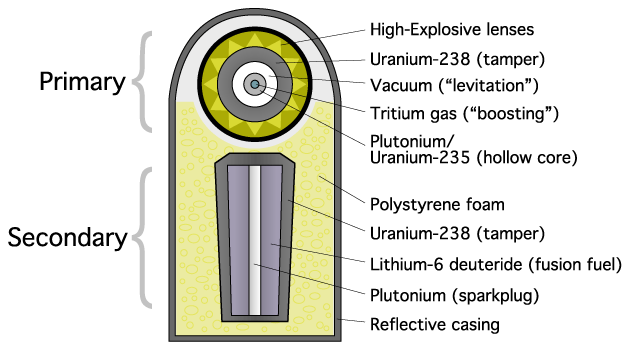
\includegraphics[scale=0.45]{./figures/Ulam_device.png}
  \caption{Schematic representation of the design of a fusion weapon \cite{WikimediaCommons2005}.}
  \label{fig:ulam_device}
\end{figure}




The basic process of detonation is as follows: The primary device triggers first and supplies x-rays, which heat the secondary device, which heats the polystyrene foam into a plasma. The Plutonium “spark plug” at the center of the fusion assembly begins to undergo fission due to the compression from the polystyrene plasma. The Lithium-6 deuteride blanket, which surrounds the plutonium spark plug, produces tritium and begins the fusion stage. The flux of neutrons from the fusion reactions causes the \ce{^{238}U} tamper to undergo fission. At this stage the device breaks apart and a detonation is complete \cite{Defense1998}. 

Fusion weapons are far more sophisticated than fission weapons, and essentially consists of three fission devices and one fusion device. It is assumed that ISIL is pursuing nuclear weapons in order to commit acts of terrorism; optimizing yield does not greatly enhance the terror of a nuclear device. Due to the complexity of the design of multistage fusion devices, it is assumed that ISIL will elect to pursue gun-type fission weapons. 






\chapter{Enabling Capabilities }

\section{Intelligence }

\subsection{Introduction}

The IC consists of sixteen distinct organizations managed by the Office of the Director of National Intelligence (ODNI) as depicted in \autoref{fig:structure_infographic}. These distinct organizations with divergent and overlapping capabilities, interests, and charters, can make a coordinated assessment of a dynamic threat like ISIL difficult. An overview of the IC and intelligence collected is provided in \autoref{app:intel}. Similar to the intelligence community (IC) reorganization following the 9/11 attacks and recommendations of the 9/11 Commission, the current threat of ISIL provides an opportunity for the IC to adapt to a dynamic threat environment and improve upon the weaknesses in IC structure and capabilities \cite{Kean2004}. Central to the U.S ability to deter ISIL from acquisitions of nuclear materials is an effective intelligence strategy to identify threats and guide response actions. 

\begin{figure}[h]
 \centering
 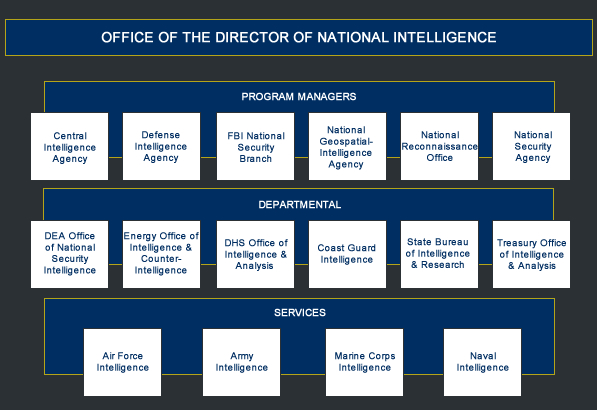
\includegraphics[trim = 0cm 0cm 0cm 0cm, clip,scale=0.7]{./figures/structure_infographic.jpg}
   \caption{Structure of the Office of the Director of National Intelligence \cite{OfficeoftheDirectorofNationalIntelligence}}
     \label{fig:structure_infographic}
\end{figure}

A basic assumption in our policy initiative is the ability of the IC to gather information through the use of radar, traditional and covert human sources, satellites, aircrafts, and ship signals \cite{Richelson2011}. This yields knowledge about the key primary, secondary and tertiary players involved, insight into the ideology and organization of ISIL, entities that might be providing it with economic or military aid, and operational details for the employment of a NW.

From the U.S. perspective, 9/11 serves as a case study to understand the shortcomings of IC, subsequent recommended changes, and possible shortcomings facing the IC with respect to ISIL. The 9/11 Report found that there are cultural and organizational factors that hinder strategic communication between U.S intelligence agencies (See \autoref{app:partners} for a discussion on strategic communication on the international level, which also applies at the inter-agency level).  Prior to 9/11, U.S intelligence agencies operated in a culture dominated by \enquote{need-to-know}, which implied that organizations were given discretion in sharing data \cite{McConnell2008}. In the context of a dynamic ISIL threat, this means that agencies often have static analyses formed from an incomplete picture and lacking a competing analysis derived from the same data. The divisions between individual agencies render them incapable of accessing, prioritizing, translating, analyzing, and relaying the information for the policymakers to respond to in a timely manner. As a result, information flow is hindered by each agency's networks and databases lacking protocols to interact with other agencies' networks and databases.  Organizational inertia, standard operating procedures, and guidelines hinder the ability to change or implement new ideas. For example, the CIA's culture of risk aversion in the 1990s was detrimental to its intelligence capabilities and prevented them from properly assessing and taking action against the rising threat of terrorism \cite{Zegart2005}.

The situation is only complicated when considering international intelligence agencies and the sharing of data. To simplify the problem, the factors considered in determining the level of cooperation and the nature of an intelligence partnership between U.S. and other countries were distilled down to the historical relationships between both parties, the country's relationship to ISIL, its military and intelligence capability, and its vulnerability and geographical proximity to ISIL. The role of international entities is gauged by the organization's functions, credibility, and past success in relaying information and promptly responding to crises.  These factors are further described in \autoref{app:intel}. 

Using the guidance in \autoref{app:intel}, a framework can be developed for information exchange between countries: 

\begin{itemize}
  \item \textbf{Level 1:} U.S. should install open information sharing with the countries in category one. During WWII, U.S. and Great Britain had joint research of the atomic bomb. This cooperation can be repeated for actions against ISIL.
  \item \textbf{Level 2:} Information sharing with category two countries should be limited to low and medium security information (see \autoref{app:intel} for further description).  
  \item \textbf{Level 3:} The U.S. should consider to have limited information sharing of low importance security information with category three countries.  
\end{itemize}

Several international organizations and treaties are in place to facilitate communication flow and prevent the spread of nuclear weapons and technology (see \autoref{app:partners}).  However, communication in these organizations organization can be a challenge, and most of the current infrastructure is designed towards state actors, not the current ISIL threat.  Although not a specific alliance against ISIL or nuclear terrorism, the five eyes agreement (see \autoref{app:intel}) can provide valuable intelligence on possible nuclear activities that ISIL may engage. This group is stable, efficient, and more nimble in intelligence collaboration than the existing international non-proliferation structure.  

\section{Military Capability}

\subsection{????? No substance for capabilities or much on current coalition efforts - Needs addressed.  Only need a little more in this section, but a more thorough overview of relevant capabilities should be in an appendix ?????}



More than 60 countries have joined the \enquote{global coalition to degrade and defeat ISIL} \cite{Drennan2014}. The member countries can choose their method and level of participation. Saudi Arabia trains and equips Syrian opposition forces. Jordan's key role will be intelligence acquiring and sharing. Germany, France, and the United Kingdom are conducting airstrikes. 

The number of countries in the coalition is growing with Obama's campaign, but the bar for inclusion is fairly low. While many countries have committed military capabilities to combating ISIL, some countries join the coalition by merely declaring their intent to contribute. All these member countries don't share the same understanding of whom the real enemy is - ISIL or the Syrian regime led by President Bashar al-Assad. For example, Turkey has urged the coalition to topple the Assad regime as a condition to provide its air bases to carry out attacks against ISIL. 

\subsection{????? I don't know what to do with this section.  It covers several area, makes unsubstantiated claims, and doesn't really coherently address the coalition or military capabilities.  I think this needs rewritten and focused.  Statements such as "the country [UK] is extra vulnerable to terrorist attacks on its nuclear installations" needs a reference and doesn't belong in this section (Perhaps an Appendix and a reference to that appendix in section 2.3.  Topic of discussion is bracketed ?????}

\subsection{????? From here... ?????}
The possibility of ISIL acquiring nuclear weapons means a stronger monitoring of nuclear-capable countries is needed. At the moment, only two handfuls of countries that have that capability. 

UK and France have been U.S.' allies even since the country launched its global fight against terrorism after the 9/11 incident. Hence, the U.S. can expect UK specifically to be its closest ally in preventing ISIL's nuclear terrorism effort. The two countries \enquote{special relationship} dated back to Churchillian era means that the U.S. can usually count on the UK for mutual support, especially considering ISIL's threats to the country is very high. UK has been ISIL's main target for terrorist attacks, and given UK's nuclear capability, the country is extra vulnerable to terrorist attacks on any of its nuclear installations. So far, UK has joined U.S.-led coalition against ISIL, nevertheless, prospect for bilateral cooperation between the two countries cannot be disregarded.

Meanwhile, France is U.S.' oldest ally and relationship remains active and friendly. France supported U.S. in various issues, however, France was skeptical when U.S. invaded Iraq after the 9/11 incident. ISIL has also posed great threats to France (being a successful nuclear energy producer and all), France can be vulnerable to attacks on its nuclear energy facilities as well as its possession of nuclear weapons stocks. France is also among ISIL's main recruitments considering France high marginalized and discontented Muslim populations. France's high ISIL threats and vulnerabilities made the country a good collaborator in effectively fighting ISIL.

Nuclear capabilities in the hand of weak or unstable government give opportunity for ISIL to acquire nuclear capabilities. Nuclear capabilities of Pakistan and its weak governance as well as security vulnerabilities is of concern to the U.S.. Looking at U.S.-Pakistan relationship, it has its ups and down. Over the decades, Pakistan has been a great ally to the U.S., but there are a few instance where the two countries were in disagreement. U.S. viewed Pakistan as its ally and threat in the country's global war on terror, in which Pakistan is seen as the \enquote{weakest link} as it continue to fail in containing act of terrorism going on in its own country. U.S. need to prop Pakistan and reduce the country's vulnerabilities of ISIL penetrations and the possibility of ISIL acquiring Pakistan's nuclear weapons.

India is also another country with nuclear weapon capability, and is mostly on the \enquote{other side} of U.S.' security policies. India, together with Russia was among the pioneers of Non-Aligned Movement (NAM), in which views on security issues tend to be divergent with the U.S.. However, as of recently, the U.S. and India have set up \enquote{global strategic partnership}, based on shared democratic values and increasing convergence of interests on bilateral, regional and global issues; key recent developments in the relationship include the rapid growth of India's economy and bilateral trade, the close links between the Indian and American computer and Internet industries, a geopolitical coalition to balance the rise of China, the weakening of U.S.-Pakistan relations, among others. U.S. has cooperated with India in area of civil nuclear, and this can be expanded to development of nuclear security hopefully in the future. However, unlike Pakistan, India believed ISIL's threats as periphery issue to the country.

In analyzing Russia as a possible bilateral partner, the two country has had strained relationship, increasingly since the economic sanctions imposed by the U.S. to Russia. Dispute between the two countries have centered on power struggle for new world order, and recently exacerbated by Russia's annexation of Crimea. The two countries have been historical rival and the Cold War has proven to be one of the expansive and stretched out power struggle between the two. However, both countries realized and agreed to maintain dialogue in several areas including terrorism. Being misaligned with Russia on ISIL and nuclear terrorism issue could be serious mistakes as Russia's nuclear capability, if not protected and are allowed to be shared in the wrong hand, could have grave catastrophic impact to global security environment.

China, another U.S.' partner and rival at times, also have nuclear capabilities. China and the U.S. has close partnership particularly in economic sector, two-way trade between the two countries is over U.S.\$590 billion in 2014 alone. Chinese Muslim Uyghur militants have been associated with ISIL and efforts to undertake terrorist attacks in China. This strengthen the need for collaboration between China and U.S.; to ensure any ISIL activities can be contained in China and the country's nuclear weapons is protected from any probability of ISIL acquiring them.

U.S. considered North Korea as grave threats and this can be further exacerbated if North Korea is presented with the opportunity to work with ISIL. The prospect of North Korea selling their nuclear weapons and missiles to ISIL cannot be discounted. However, the possibility of U.S. and North Korea to cooperate in hampering this issue is not viable. The U.S. need to come up with initiatives to solve this problem.

Iran and U.S. shared a common enemy factor in terms of ISIL. As the nuclear talks between the two countries are being hashed out, both countries have committed on fighting ISIL together. This can be a good opportunity for U.S. to combat ISIL more effectively as U.S. cannot disregard Iran's influence and role in Iraq's security landscape and their fight against ISIL.
Meanwhile, collaborating with Israel is considered a gray area and not clear-cut as it seems. Israel has been known to voice their support of ISIL, keeping in line with ISIL's common enemy with Israel i.e. Iran. As U.S. and Israel have been a strong ally in the Middle East region, this fact presented a conundrum to the U.S..

The U.S. may find other allies in the Middle East region, however, the region is deeply divided in their positions against the ISIL. Although most Middle Eastern countries sees ISIL as a serious threat to the region and its people, some still supported ISIL, if not openly but explicitly. U.S. has worked closely with Jordan, with the U.S. creating a U.S.\$5 billion counterterrorism partnership fund with Jordan and other countries (Libya, Lebanon, Syria) that are considered on the \enquote{frontlines} of U.S.' fights against ISIL.

The U.S. can find allies in European countries as well, as the region is facing \enquote{recruitment} threats from ISIL. Thousands of Europeans have been recruited by ISIL to fight jihad cause in ISIL's territories. ISIL is also setting up bases in a number of European countries, expanding its influence beyond the Middle East region. The U.S. can identify these countries and create cooperation efforts in order to effectively eliminate ISIL.

\subsection{????? ...to here. ?????}







\section{Post-Detonation Forensics Methods}

\subsection{????? Need short paragraph discussion on pre-detonation nuclear forensics. ?????}

The goal of post detonation forensics is to determine the design, composition, and origin of a nuclear weapon. To assist in the attribution process, there exists a distributed network of monitoring stations which measure different signals which would confirm the occurrence and characteristics of a nuclear detonation. These stations include: over 170 seismic monitoring devices, six underwater (hydroacoustic) and 5 land systems which monitor sound waves, and 60 surface stations which measure infrasound (ultra-low-frequency) \cite{Lane2012}. The location of detonation and the yield of the nuclear device may be estimated from an analysis of these signals. In the hours and days that follow detonation, measurements of the radionuclide composition near the blast zone and in the plume of gas and dust released into the upper atmosphere allow conclusions to be drawn concerning the efficiency of the device, the weight of the fuel (i.e. the level of sophistication), whether the fuel was plutonium or uranium, how the fuel was created, and whether or not DT fusion occurred (based on the known cross-sections of 14 MeV neutrons with the surrounding environment) \cite{Davis2011}. Additionally, there exists a vast orbital infrastructure which monitor for optical, X-ray, gamma-ray, and neutron emission characteristic of nuclear detonations; the exact capabilities of these systems is classified \cite{1446400}. 

\subsection{Timescale for data processing and response}

Reference on Drive: Forensic questions you can answer (in the fission folder).

If nuclear material is intercepted before detonation, an analysis of the enrichment and contaminants may be achieved at the National Labs (Oak Ridge, Los Alamos). On the scale of weeks to months, it is possible to discern the age of the material post fabrication by analyzing the micro-structure, activity, and isotopic composition. Immediately following detonation, the timescale of analysis relies on how quickly radiation monitoring equipment may be delivered to the blast site and how quickly samples are gathered and shipped back to one of 16 radiological facilities equipped to perform nuclear forensics \cite{1446400}. Airplanes capable of sampling large volumes of the dust and gas (Xenon) in the plume generated by the detonation must be performed within 1-2 days of the detonation and may indicate the composition, efficiency, and sophistication of the device. Analysis of materials taken from the ground near the detonation point will take 1-2 weeks to analyze and will confirm and refine the findings of atmospheric monitoring. The identification of the origin of the weapon will depend largely on what is presently known about the yield, sophistication, and efficiency of weapons in global stockpiles. What is exactly known of the capabilities of weapons designed outside of the United States is classified \cite{Glasstone_1964}. Given quick access to the nuclear blast site and a somewhat thorough understanding of the nuclear capabilities of other sovereign powers, the technical analysis of the origin and design of a nuclear blast would be available within 3-10 days, depending on the availability of data. Ongoing research is aimed at developing LIBS technologies which may reduce the nuclear forensics timeline with rapid (\textless 15 hours) debris dissolutions techniques, or techniques which do not require the dissolution of collected debris \cite{Condron}. 


\section{Detection technologies }

\subsection{????? Recommend developing short (~1 page or less) overview of some of the high level considerations involved in detecting nuclear material, limitations, and current programs.  Place the remainder of the material, basically what is included here, into an Appendix.  Did not grammar review.   ?????}

\subsection{Fission Weapons}
 
   \subsubsection{Passive Signals}

Passive signals for nuclear materials include the gamma rays that are given off during natural radioactive decay of the material, and neutrons that result either from spontaneous fission or (\(\alpha\),n) nuclear reactions (the \(\alpha\) particle comes from natural \(\alpha\) decay). The two most likely and common types of material that could be used for a nuclear weapon are highly enrich \ce{^{235}U} and highly enriched \ce{^{239}Pu}, and so these materials will be considered for passive detection. Weapons grade Uranium has a very low rate of released neutrons, and so detection by gamma rays would be recommended. Weapons grade Plutonium releases both, a large amount of neutrons and gamma rays and so both methods of detection are possible. 

The time needed to get acceptable detection by use of neutron and gamma counters varies based on distance and materials. \autoref{fig:det_time} shows an conservative estimate of the distance a mobile detector would need to be to get confirmation data that is 5 standard deviations above the background radioactivity. 


\begin{figure}[h]
 \centering
 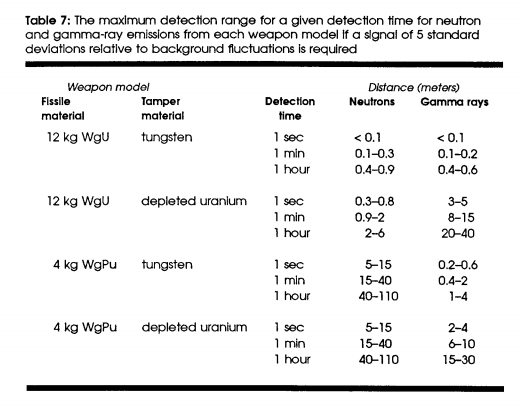
\includegraphics[trim = 0cm 0cm 0cm 2cm, clip,scale=0.6]{./figures/det_time.png}
   \caption{Table of distance and time needed to detect Weapons Grade  material with a tamper, where detection is considered when the counts are 5 standard deviations above the background. \cite{Fetter1990}}
     \label{fig:det_time}
\end{figure}


Passive gamma detection of weapons grade plutonium and uranium with a tungsten tamper are unlikely as the distance for detection is too small, even for a long detection count of 1 hour (\autoref{fig:det_time}). Passive neutron detection of weapons grade uranium is also unlikely for the same reasons. 


While the other weapon models have a fair distance of detection for a short time, the data does not take into account, additional shielding. To prevent detection by neutrons for a one minute detection period and one meter distance from the source, only 20 cm thick layer of lithium hydride would be needed \cite{Fetter1990}. To counter this, long detection period (\textgreater 10 minutes) \cite{Fetter1990} would be needed. Avoid detection of the gamma rays is significantly more difficult. The most likely and effective material to block gamma rays is lead. In order to bring the required detection period from 1 meter away to a time greater than 5 minutes, at least 100 kg of lead would be needed (see \autoref{fig:shield_time}).


\begin{figure}[H]
 \centering
 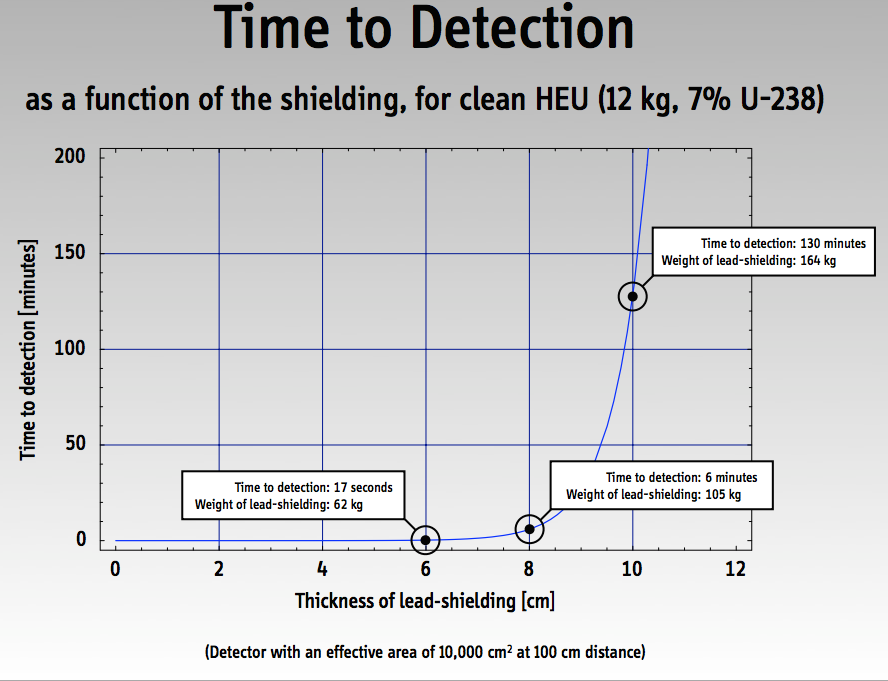
\includegraphics[trim = 0cm 0.1cm 0cm 0cm, clip,scale=0.4]{./figures/shield_time.png}
   \caption{Time needed to reach a gamma count of highly enriched uranium (HEU) 5 standard deviations above the background for a given lead shield thickness \cite{Glaser2007}.}
     \label{fig:shield_time}
\end{figure}



If short detection time periods are needed, then it is unlikely that passive signals could be effectively utilized. If longer detection time are able to be done, then gamma detection of weapons grade plutonium and uranium with a depleted uranium tamper are possible with distances greater than or equal to 1 meter away. However, the requirement of the tamper material to be depleted uranium makes this method of detection highly not recommended, as or tamper materials such as tungsten are not significantly less likely to be used. 



\subsubsection{Active Signals}


% \myparagraph{Introduction to Active Interrogation}
\textbf{Introduction to Active Interrogation}


Active interrogation is a technique where an interrogating beam of neutrons or x-rays is used to scan a container in order to excite a response signal in special nuclear material. There are many different methods of active interrogation, which involve scanning the sample with different types of particles and measuring the resulting x-rays or gamma rays emitted by the material which was scanned.

Active interrogation can accurately identify special nuclear material. Furthermore, given the many methods of active interrogation, it is harder to shield against than passive detection.

While, active interrogation is a very good way to detect shielded nuclear material that is undetectable by passive interrogation, it does have two primary problems. The first, comes from the problem of illegal immigrants using cargo containers to enter a country through its ports. If the dose from active interrogation is high enough, the interrogation could result in the deaths of any potential stowaways \cite{Morse2014}. The second, is a logical conclusion that can be drawn from the definition of active interrogation. Namely, it involves shooting a beam at a target and waiting for a reaction. This obviously takes longer than simply measuring if any radiation comes off of a container. Thus, it is very likely not possible to use active interrogation on every container at a port, without slowing down commerce.

\textbf{Nuclear Resonance Fluorescence}

Nuclear Resonance Fluorescence is a method of active interrogation that involves hitting a target with high energy X-rays. This causes special nuclear material to enter an excited state, which will de-excite and give off a fluorescence gamma ray which can be detected. These fluorescence gamma rays are unique to each isotope allowing for positive identification \cite{Morse2014a}. The signatures expected from \ce{^{235}U} and \ce{^{239}Pu} are given in \autoref{tab:fluor_gammas}.

The main benefit of this method of active interrogation is that it works through several inches of steel or lead and several feet of hydrogenous material, which passive detection does not \cite{PhysRevC.78.041601}. Another interesting benefit is that this method of active interrogation can detect not only fissionable materials, but also any isotope larger than helium \cite{Bertozzi2005}.

This method of interrogation is able to function with very few counts. For example if the material gives of 20 counts, and the detector threshold is set at 17, meaning it alerts whoever is monitoring it when it receives 17 counts, this method has an efficiency of 99\% and a false positive rate of only 1\% \cite{Chichester2009}. 

\begin{figure}[h]
 \centering
 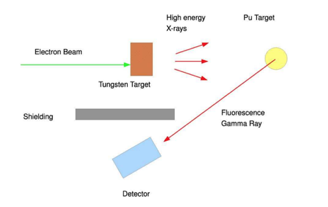
\includegraphics[trim = 0cm 0cm 0cm 0cm, clip,scale=0.7]{./figures/NRF_setup.png}
   \caption{A typical set-up for  a nuclear resonance fluorescence system \cite{Morse2014a}.}
     \label{fig:NRF_setup}
\end{figure}




% Please add the following required packages to your document preamble:
% \usepackage{multirow}
\begin{table}[H]
\centering
\begin{tabular}{|c|c|c|}
\hline
Isotope                 & Transition    & Statistical Significance \\ \hline
\multirow{9}{*}{\ce{^{235}U}}   & 1656.23(80)   & 5.8                      \\ \cline{2-3} 
                        & 1687.26(33)\footnotemark[1]  & 10.2                     \\ \cline{2-3} 
                        & 1733.60(22)\footnotemark[1]  & 56.4                     \\ \cline{2-3} 
                        & 1769.16(28)\footnotemark[2] & 9.3                      \\ \cline{2-3} 
                        & 1815.31(22)\footnotemark[2] & 19.9                     \\ \cline{2-3} 
                        & 1827.54(23)   & 13.3                     \\ \cline{2-3} 
                        & 1862.31(20)   & 20.1                     \\ \cline{2-3} 
                        & 2003.32(25)   & 14.5                     \\ \cline{2-3} 
                        & 2006.19(31)   & 7.2                      \\ \hline
\multirow{12}{*}{\ce{^{239}Pu}} & 2040.25(21)   & 5.8                      \\ \cline{2-3} 
                        & 2046.89(31)   & 4.2                      \\ \cline{2-3} 
                        & 2135.00(37)\footnotemark[1]  & 3.5                      \\ \cline{2-3} 
                        & 2143.56(13)\footnotemark[1]  & 9.7                      \\ \cline{2-3} 
                        & 2150.98(31)\footnotemark[1]  & 4.2                      \\ \cline{2-3} 
                        & 2289.02(25)   & 6.2                      \\ \cline{2-3} 
                        & 2423.48(22)\footnotemark[2] & 7.2                      \\ \cline{2-3} 
                        & 2431.66(25)\footnotemark[2] & 6.3                      \\ \cline{2-3} 
                        & 2454.37(26)   & 6.2                      \\ \cline{2-3} 
                        & 2460.46(37)   & 4.7                      \\ \cline{2-3} 
                        & 2464.60(30)   & 5.7                      \\ \cline{2-3} 
                        & 2471.07(34)   & 4.6                      \\ \hline
\end{tabular}
\caption{Fluorescence Gamma Rays Given off by Isotopes of Concern \cite{PhysRevC.78.041601}.}
\label{tab:fluor_gammas}
\end{table}

\footnotetext[1]{Line pairs which are separated by 46.2 keV implying that one of the decays goes to a ground state while the other is to an excited state with an energy of 46.2 keV \cite{Bertozzi2005}. Furthermore, \ce{^{233}U} and \ce{^{237}Np} are not included here because of the low probability that they would be used in a device obtained by ISIL.}

\footnotetext[2]{Another set of line pairs separated by 46.2 keV implying that one of the decays goes to a ground state while the other is to an excited state with an energy of 46.2 keV \cite{Bertozzi2005}.}




\textbf{Neutron Interrogation}

Neutron interrogation involves hitting a target with a pulsed beam of neutrons in order to induce fission in target fissile material. Once fissions occurs, prompt and delayed neutrons and photons are emitted from the sample and may be detected. The characteristic energies of the neutrons and photons reveal the identity of the material \cite{Chichester2009}.  \autoref{fig:Chichester_timing}  shows the general pattern of responses to this type of interrogation while representative count rates for special nuclear material shielded by wood. Furthermore specific signatures to that can be expected from \ce{^{235}U} and \ce{^{239}Pu} can be found in \autoref{tab:neutron_signatures}.

The primary advantage of this technique is is that the systems are very small (\textless\ 0.2 m\(^3\)), light weight (\textless\ 12 kg), and use very little power (\textless\ 50 W) \cite{Chichester2009}.  Another major benefit is that research indicates this method will not subject the cargo to an excessive dose of radiation \cite{Hall2007}.  One major downside of this method is that it seems like research is still being conducted to determine if this method will work for a full size ago container \cite{Hall2007}.  A second major downside is that current technology requires the sample to be less than a meter from the detector, approximately 91.4 cm \cite{Hall2007}. A major technical downside of this technology is that, because it works by inducing fissions, it is only able to detect fissionable material.



\begin{figure}[h]
 \centering
 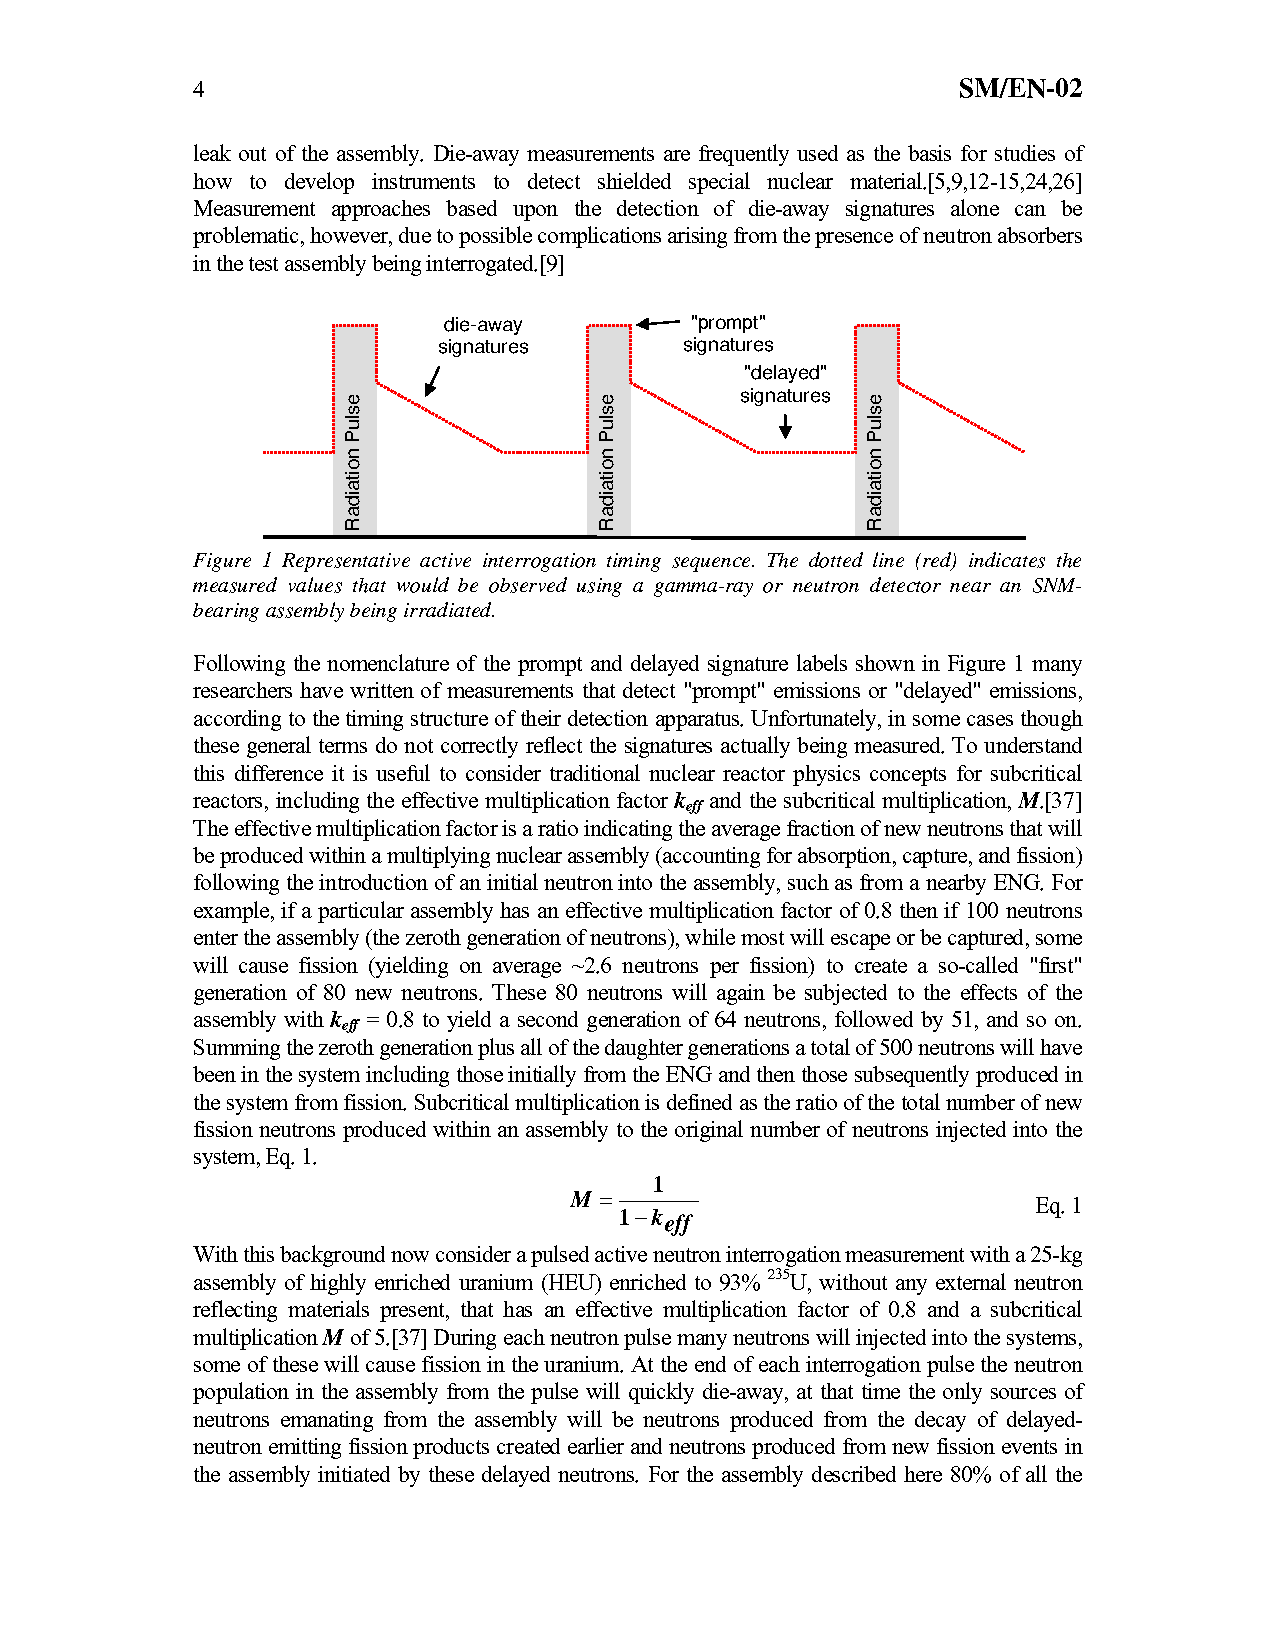
\includegraphics[trim = 5cm 18.7cm 5cm 5cm, clip,scale=1]{./figures/Chichester_timing.pdf}
   \caption{Representative pattern for pulsed neutron beam and when specific signatures can be expected \cite{Chichester2009}.}
     \label{fig:Chichester_timing}
\end{figure}


\begin{figure}[h]
 \centering
 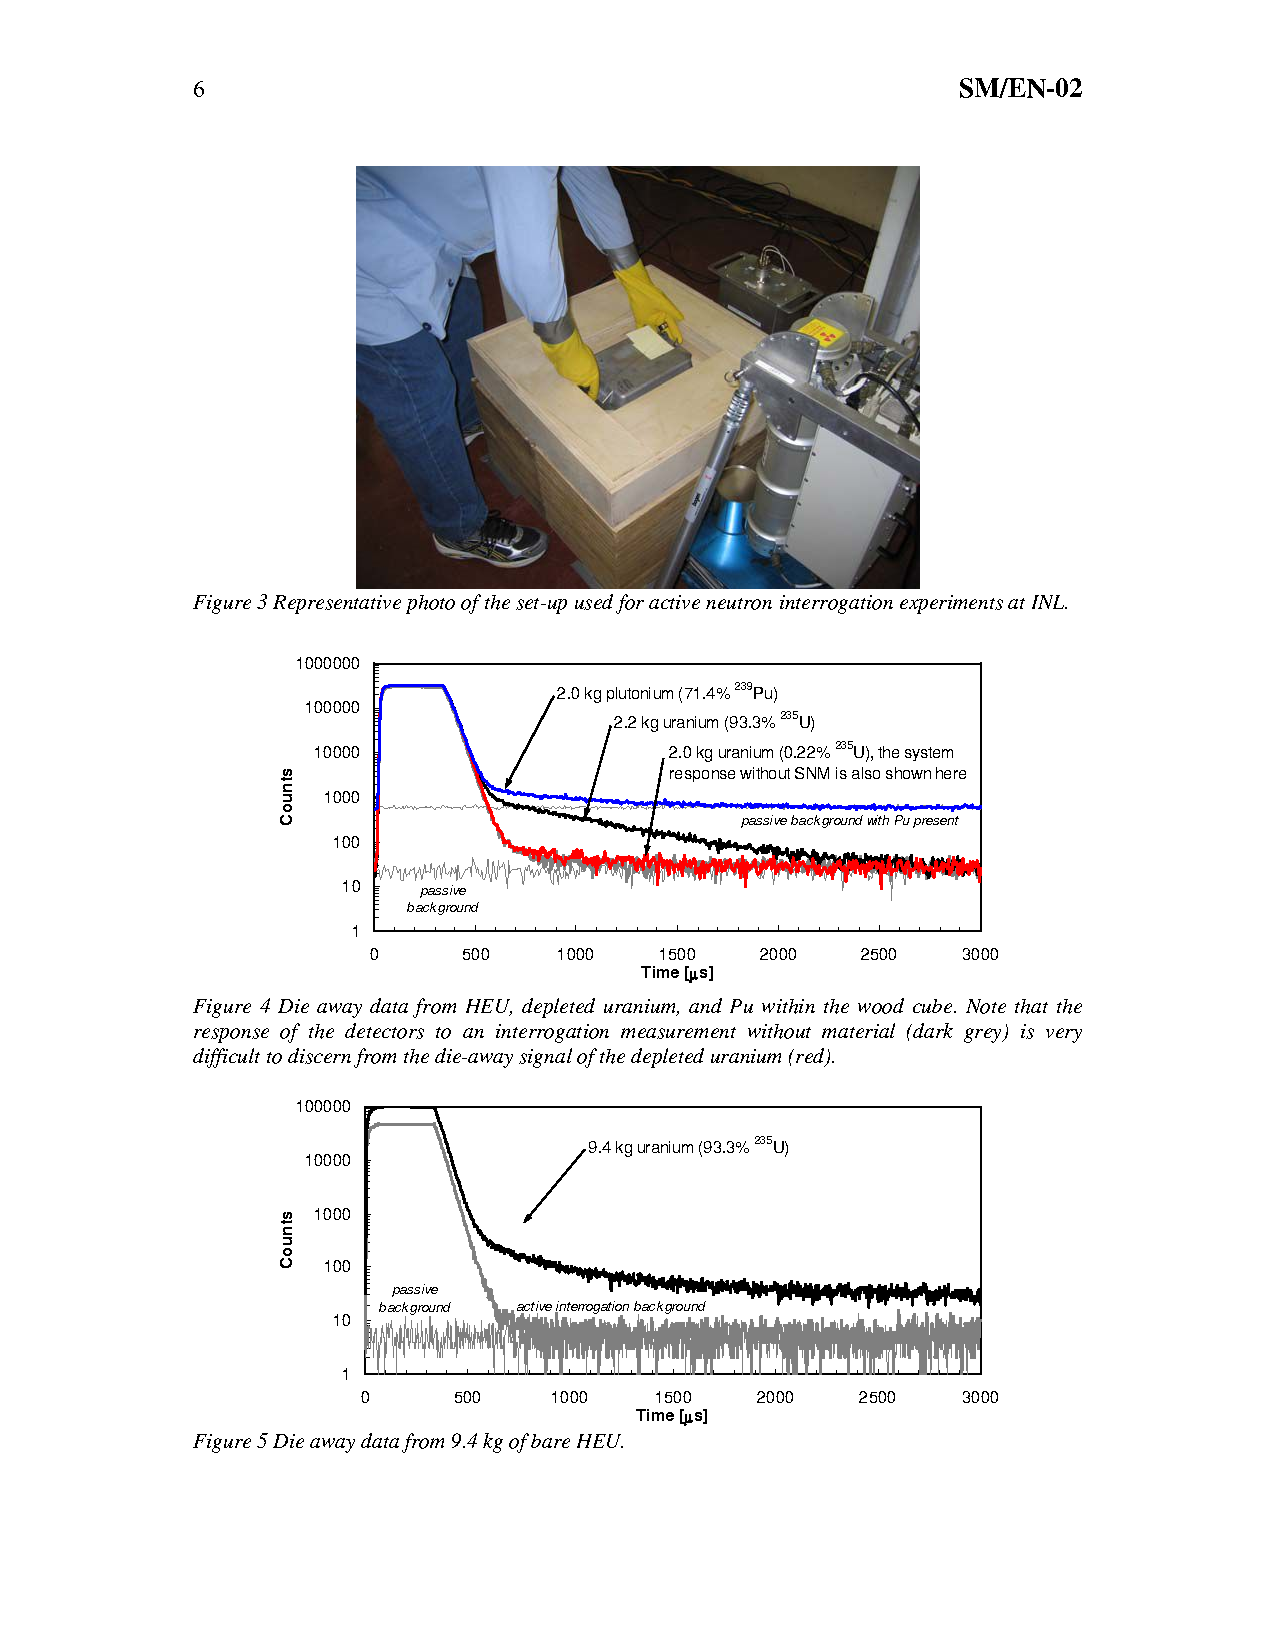
\includegraphics[trim = 3cm 11.3cm 3cm 10.5cm, clip,scale=1]{./figures/Chichester_counts.pdf}
   \caption{Counts over time for HEU, depleted uranium, and Pu in a wooden cube \cite{Chichester2009}.}
     \label{fig:Chichester_counts}
\end{figure}



As can be seen in \autoref{fig:Chichester_counts}, counting times necessary to identify samples are not incredibly long and can be under a minute \cite{Chichester2009}.




\begin{table}[H]
\centering
\begin{tabular}{|c|c|c|}
\hline
Parameter                                                                                                                & \ce{^{235}U}                                                                                               & \ce{^{239}Pu}                                                                                               \\ \hline
\begin{tabular}[c]{@{}c@{}}Average Prompt Neutron Yield (multiplicity)\footnotemark[4]\\ (prompt neutrons per fission)\end{tabular}   & \begin{tabular}[c]{@{}c@{}}2.43 (thermal) \\ 2.57 (fission spectrum) \\  4.6 (14 MeV)\end{tabular} & \begin{tabular}[c]{@{}c@{}}2.87 (thermal) \\  3.09 (fission spectrum) \\  4.9 (14 MeV)\end{tabular} \\ \hline
\begin{tabular}[c]{@{}c@{}}Average Prompt Neutron Energy\footnotemark[5]\\ (MeV)\end{tabular}                                         & \begin{tabular}[c]{@{}c@{}}1.935 (thermal) \\  2.03 (14 MeV)\cite{PhysRevC.69.034607}\end{tabular}                       & \begin{tabular}[c]{@{}c@{}}2.010 (thermal) \\  2.19 (14 MeV)\cite{PhysRevC.69.034607}\end{tabular}                        \\ \hline
\begin{tabular}[c]{@{}c@{}}Average Prompt Photon Yield\\ (prompt photons per fission)\end{tabular}                       & 6.60\(\pm\)0.2 (thermal)\cite{Valentine2001}                                                                            & 7.06\(\pm\)0.2 (thermal)\cite{Valentine2001}                                                                             \\ \hline
\begin{tabular}[c]{@{}c@{}}Average Prompt Photon Energy\footnotemark[6]\\ (MeV)\end{tabular}                                          & 0.97\(\pm\)0.04 (thermal)\cite{Valentine2001}                                                                           & 0.95\(\pm\)0.04 (thermal)\cite{Valentine2001}                                                                            \\ \hline
\begin{tabular}[c]{@{}c@{}}Average Delayed Neutron Yield (multiplicity)\footnotemark[4]\\ (delayed neutrons per fission)\end{tabular} & \begin{tabular}[c]{@{}c@{}}0.0158 (thermal) \\  0.0165 (1.45 MeV)\end{tabular}                     & \begin{tabular}[c]{@{}c@{}}0.0061 (thermal) \\  0.0063 (1.45 MeV)\end{tabular}                      \\ \hline
Average Delayed Neutron Energy (MeV)                                           & 0.43                                                                                               & 0.4                                                                                                 \\ \hline
\begin{tabular}[c]{@{}c@{}}Average Delayed Photon Yield\footnotemark[7]\\ (delayed photons per fission)\end{tabular}                  & \begin{tabular}[c]{@{}c@{}}0.613 (short period) \\  3.31 (long period)\end{tabular}                & \begin{tabular}[c]{@{}c@{}}0.608 (short period) \\  3.26 (long period)\end{tabular}                 \\ \hline
Average Delayed Photon Energy (MeV)\footnotemark[8]                                         & 0.96                                                                                               & 0.98                                                                                                \\ \hline
\end{tabular}
\caption[Signatures from Active Neutron Interrogation \cite{Chichester2009}]{Signatures from Active Neutron Interrogation \cite{Chichester2009} \footnotemark[3]}
\label{tab:neutron_signatures}
\end{table}

\footnotetext[3]{Parentheses following certain values indicate fissions induced by neutrons of that specific energy}
\footnotetext[4]{Yields change based on the energy of the neutron that causes the fission}
\footnotetext[5]{Increases of approximately 4\% are expected for average neutron fission energies when going from thermal-neutron induced fission to fission-spectrum induced fissions}

\footnotetext[6]{Less than 2\% of these photons have energies larger than 2 MeV}
\footnotetext[7]{Delayed photon yields were measured over two counting periods. A short one, 0.2 s \textless t \textless 0.5 s and a long one, 0.2 s \textless t \textless 45 s.}
\footnotetext[8]{Energies averaged over the long counting period. Less than 1.8\% of the photons have energies greater than 2.3 MeV}



\subsection{Strategies for detecting RDD}
 
\subsubsection{Passive Signals}

The types of radioactive signals emitted from the \enquote{top 10} materials listed in \autoref{sec:RDD} are summarized here in \autoref{tab:RDD_signals}.  These passive radioactive signatures were acquired by various detection methods, with the most typical being the High Purity Germanium (HPGe) detectors and associated detector signal amplification and diagnostic tools \cite{Glaser2007}.  For each isotope, the radiation types are listed, some of primary energy levels for emitted particles based on laboratory testing results or other available references are included, and the total mass of a pure source which emits 1 petabecquerel (10\(^{15}\) Bq) of activity was calculated for inclusion. 




\begin{table}[h]
\centering
\begin{tabular}{|l|c|l|l|}
\hline
\multicolumn{1}{|c|}{Isotope} & \multicolumn{1}{c|}{Type of emission} & \multicolumn{1}{c|}{\begin{tabular}[c]{@{}c@{}}Energy of emission \\ peak(s) {[}keV{]}\end{tabular}} & \multicolumn{1}{c|}{\begin{tabular}[c]{@{}c@{}}Material mass required \\ for producing  1 PBq \\ of Activity {[}g{]} (lbs)\end{tabular}} \\ \hline
\ce{^{241}Am}                         & \(\alpha\)                                 & 59.54                                                                                               & 7871.27 (17.353)                                                                                                                         \\ \hline
\ce{^{137}Cs}                         & \(\beta\), \(\gamma\)                            & \begin{tabular}[c]{@{}l@{}}661.67 \\ 383.85 \\ 356.02 \\ 302.9 \\ 276.4 \\ 80.9\end{tabular}        & 312.06 (0.688)                                                                                                                           \\ \hline
\ce{^{131}I}                          & \(\beta\)                                  & 606                                                                                                 & 0.22 (0.0005)                                                                                                                            \\ \hline
\ce{^{192}Ir}                         & \(\beta\), \(\gamma\)                            & 1459.7                                                                                              & 2.93 (0.006)                                                                                                                             \\ \hline
\ce{^{90}Sr}                          & \(\beta\)                                  & 546                                                                                                 & 195.56 (0.431)                                                                                                                           \\ \hline
\ce{^{3}H}                            & \(\beta\)                                  & 18.6                                                                                                & 2.81 (0.006)                                                                                                                             \\ \hline
\ce{^{60}Co}                          & \(\gamma\)                                 & \begin{tabular}[c]{@{}l@{}}1173.24 \\ 1332.5\end{tabular}                                           & 23.88 (0.053)                                                                                                                            \\ \hline
\end{tabular}
\caption{Summary of Radioactive Signal Emissions for RDD Isotopes of Concern}
\label{tab:RDD_signals}
\end{table}



The NRC defines LD50(30) to be the dose of radiation expected to cause death to 50 percent of an exposed population within 30 days (LD 50/30). Typically, the LD 50/30 is in the range from 400 to 450 rem (4 to 5 Sv) received over a very short period \cite{U}.  From this metric, the dose of 400 rem will be selected for evaluation here, and would require a very large source emission of radiation - typically one much larger than the practical release and yield of a RDD - and it will not occur over a very short period.

For passive detection of radiological materials, including isotope identification, gamma ray spectroscopy of radioactive emissions can be utilized with the development and deployment of aerial vehicle mounted radiological survey detectors \cite{Security2012}.



 
\subsubsection{Shielding of Radioactive Materials}

Of the radiation types mentioned: alpha, beta, and gamma, the gamma emitters are by far the farthest penetrating, most energetic, radioisotope emitters listed.  The shielding suggested will merely attenuate the energy levels of the gamma emissions, but in essence the emission passes through the shielding and continues on its travel through the medium. \autoref{fig:shielding_reqs} shows relative stopping distances in materials for given radiation types. Alphas, although they can be very energetic upon initial release from the source, are very large particles in comparison to the surroundings.  It is more likely that the 2+ charged alpha ion will interact with matter than the other radiation types, even as depicted a piece of paper is sufficient shielding material to attenuate alpha emissions. 


\begin{figure}[h]
 \centering
 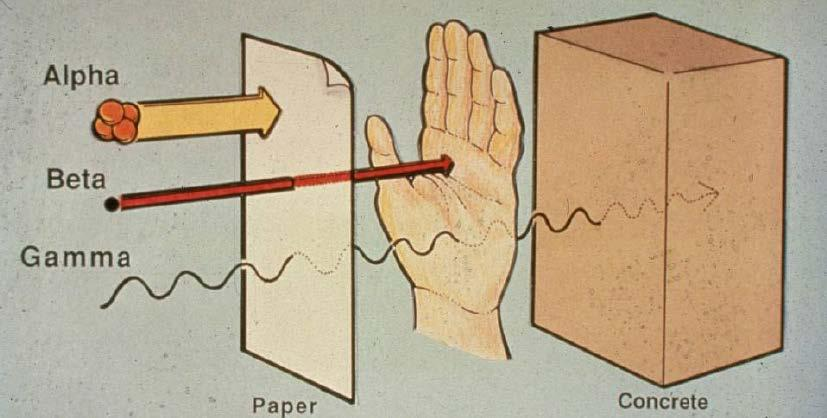
\includegraphics[trim = 0cm 0cm 0cm 0cm, clip,scale=0.5]{./figures/shielding_reqs.jpg}
   \caption{Schematic representation of the shielding requirements of alpha, beta, and gamma radiation \cite{Hallenbeck1994}. }
     \label{fig:shielding_reqs}
\end{figure}

\subsubsection{????????  This section needs MASSIVE cleaning up ????????}




\section{Etc...}




\chapter{What can be done - possibilities for our policy to be implemented}

\section{Logic Trees}

Waiting on Julie

The logic tree can be seen in \autoref{fig:logic_tree}.

\includepdf[angle=270, pagecommand={\thispagestyle{fancy2}\null\vfill\captionof{figure}{Non-linear Logic Tree}\label{fig:logic_tree}}, scale=0.85]{./figures/NucSec_Logic_Model.pdf}


\subsubsection{????????  Orphan Policy Statements, need polishing and integration ????????}

This report will concentrate on overcoming the complexities in the IC organizational structure to facilitate information sharing. The policy recommendation is a two-pronged strategy that addresses intelligence sharing and analysis on both the domestic and international aspects. The goal for the intelligence community is to foster efficient coordination by improving the flow of information among intelligence organizations, changing the \enquote{need-to-know} basis culture of information sharing, and promoting integration across the organizations to provide time-pertinent. In terms of the international side, the policy will revolve around identifying countries and international bodies the U.S is willing to share information with and to what extent the parties will be involved in the process of intelligence analysis and policy formation.

\subsection{Intel Policy Solution}

The best means of counteracting this fragmentation is to develop a more integrated system with the ODNI at the helm of this  centralized structure. The Office of the Director of National Intelligence should be allowed more authority to dictate the management of information across agencies.  To increase the coordination and familiarity with other agencies in the intelligence community, personnel should do rotations in each of the agencies. This way, it promotes cross-agency relationships and personnel become better equipped at sharing and comparing methods of collecting and analyzing information.  Agencies should be less structured on rules and regulations and instead focus on how to best adapt to changing circumstances. A combination of minimal oversight and conflicting missions due the independent nature of these agencies \cite{Zegart2005} require that ODNI implement a uniformity of standards to decrease costs and simplify the flow of information. 

\subsection{Military Policy Solution}
 
As ISIL carves its traction in Iraq and Syria, the two countries become an immediate concern for help by the U.S.. Strengthening Iraq and Syria could be among the first line of defense against ISIL. As U.S. has an improving bilateral relations with Iraq, Iraq become an easier partner for U.S. to work with in reigning ISIL. The Strategic Framework Agreement for a Relationship of Friendship and Cooperation between the U.S. and the Republic of Iraq guides the overall political, economic, cultural, and security ties with Iraq.  This agreement is designed to help the Iraqi people stand on their own and reinforce Iraqi sovereignty, while protecting U.S. interests in the Middle East. 

However, the country's relation with Syria is not black-and-white as we would like it to be. The U.S.-Syria relationship is negative after having suspended diplomatic relations in 2014. The U.S. has also imposed economic sanction to Syria since 2004 due to the country's involvement in harboring terrorist groups and the meddling of Lebanon's political affairs including the assassination of Lebanese Prime Minister Rafik Hariri. The U.S. deeply opposed to the ongoing Syrian Civil war and President Bashar al-Assad's regime, specifically regarding the country's use and stockpile of chemical and biological weapons. The U.S. has floated the idea to train the Syrian military opposition, and even considering to train the Syrian military itself in order to fight ISIL, nevertheless, President Assad viewed the proposal as infringing on their country's sovereignty. Despite the two countries differences, they actually both share a common enemy, and it is hope this fact can be harnessed to U.S.' advantage.


\subsubsection{????????  Orphan Policy Statements, need polishing and integration ????????}


\section{Target links in the logic tree}

\subsection{Pillars of nuclear technology acquisition }

There are three approaches to disrupting ISIL's operations that will be particularly important in ensuring that ISIL does not acquire a nuclear device:

\begin{itemize}
  \item Disrupt ISIL cash flow
  \item Rollback ISIL territorial gains
  \item Counteract ISIL's draw to foreign fighters
\end{itemize}

\subsubsection{Disrupt Cash Flow}

\subsubsection{???????  Need better source for ref [1]    ???????}

ISIL's principal source of income is derived from control and sale of oil, which brings in about \$1 million a day [1]. Additional funds come from kidnap for ransom, extortion, criminal activities, and a small amount from external donations. 

[1]  Brookings Institution, Summarizing speech by David Cohen, undersecretary for terrorism and financial intelligence at DoT

A new report by Financial Action Task Force (an international body) finds that it is unclear whether ISIL's revenue collection will be sustainable over time, and that ISIL will have to gain more territory to remain financially viable \cite{TheEditorialBoard2015,Report2015}.

ISIL employs an estimated 30,000 fighters, including 19,000 foreign fighters from 90 different countries, paying them roughly \$350-\$500 a month. This leads to a total payroll cost of \$10 million per month. ISIL also tries to bolster its appeal by providing public services, including electricity, to people in its territory. 

Current U.S. strategy is to:

\begin{enumerate}
  \item Disrupt ISIL revenue streams
  \item Restrict ISIL access to international financial systems
  \item Target ISIL leaders and supporters with sanctions
\end{enumerate}



\textbf{Disrupt ISIL Revenue Streams}

In the current oil market, diminished profits from selling oil may make ISIL more dependent on external donations. As need for this arises, it is important to focus on these external sources. Saudi Arabia and UAE are becoming more effective at preventing funding of terrorist organizations by their citizens, but Kuwait and Qatar remain permissive jurisdictions. More needs to be done by these states to enforce their newly passed laws against financing terrorism, and the U.S. can help them do this through State Department and other training. It is important to note that these Gulf states have an interest in stopping ISIL – ISIL has periodically targeted Qatar and its Ministry of Foreign Affairs. \subsubsection{???????? THIS PARAGRAPH NEEDS SOURCES   ?????????} 

Extortion and illicit taxation are large, internally sustainable methods of funding for ISIL. Before capturing Mosul, ISIL was already earning \$12 million a month in the city from these methods. A sophisticated ISIL taxation system has been created on the main highway between Jordan and Baghdad that replaces the government's import tax by charging a reduced rate for goods transported into the capital. ISIL does this throughout Iraq and Syria, and ensures its survivability by gaining tax income while charging low rates to Sunni truckers and other Sunnis to curry favor. Truly eroding this source of funding means breaking ISIL's hold over the territory. This is highly unlikely to happen without sophisticated ground forces following up on the airstrikes. 

\subsubsection{???????  Need better source for ref [1]  below  ???????}


Disabling ISIL oil revenue is more complicated than it might seem. ISIL has been focused on establishing a durable internal market for oil, ensuring they have a reliable source of fuel for its fleets and also establishing dependence from the local population on its cheap oil. Recent airstrikes have targeted the oil at its source, but might be better served by targeting means of transportation and sale. Syrian rebels have pointed to this as a major error in targeting, as it disrupts oil supply to power generators and local facilities, allowing ISIL to pass the blame on to the U.S. (who they call \enquote{the crusaders}) when the electricity system fails. One difficulty in targeting the means of transportation and sale is that oil is transported in tanker trucks and oil drums, and most of the transactions are in cash, making them hard to track. One policy priority should be providing large quantities of diesel fuel and oil for generators in opposition areas of northern Syria [1].
A final recommendation is to put more intelligence resources toward detecting ISIL fundraising efforts through modern communication networks (social media) \cite{Report2015}.

\textbf{Restrict ISIL access to international financial systems}

The U.S. should share practical information and intelligence at an international level, both spontaneously and on request, to effectively disrupt international financial flows \cite{Report2015}.

Operating entirely in cash is risky and cumbersome – it will be important for ISIL to access the banking system in Syria, Iraq, and internationally. Access to the international banking system is also important for ISIL to fund external operations, including operatives who may be tasked with attacking the U.S. homeland. 

There are many bank branches located in the territory where ISIL operates. DoT should aim to prevent ISIL from using these bank branches. 

The private sector is also important in these efforts. The Bank Secrecy Act allows private companies to give DoT insight into financial activity in areas where ISIL operates. 

\textbf{Target ISIL leaders and supporters with sanctions}

The U.S. should request countries to proactively identify individuals and entities for inclusion in the UN al-Qaeda Sanctions Committee list \cite{Report2015}.

 \subsubsection{???????? Say more about this, what is this list??   ?????????}

In particular, sanctions will be levied against ISIL leadership, supporters, and financial facilitators. Effective use of sanctions against the CFO-like figures who manage ISIL funding networks will frustrate ISIL's ability to raise money and recruit fighters \cite{Cohen2014}.

\subsubsection{Rollback ISIL territorial gains}

Airstrikes and other military interventions should be focused in areas that have oil reserves, mineral resources, ex-nuclear facilities, current nuclear facilities, and sources of electricity, heavy machining capabilities, and explosives production. We will present a series of maps to graphically display key areas where preventing and rolling back ISIL advances should be a priority.

Note to Red Team: I would like to integrate this into one or a few maps. I'm not sure how exactly to do this (so if anyone does let me know). If you think that's a good idea, I'll work on it over the next couple of weeks.



\begin{figure}[h]
 \centering
 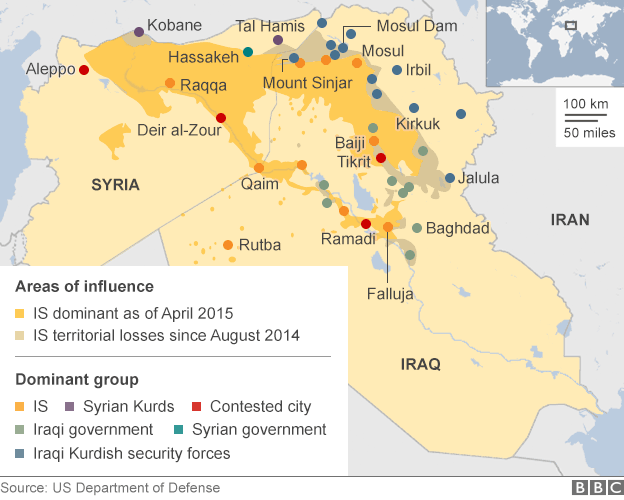
\includegraphics[trim = 0cm 0cm 0cm 0cm, clip,scale=0.6]{./figures/current_territory.png}
   \caption{Current ISIL Territory}
     \label{fig:current_territory}
\end{figure}



\begin{figure}[H]
 \centering
 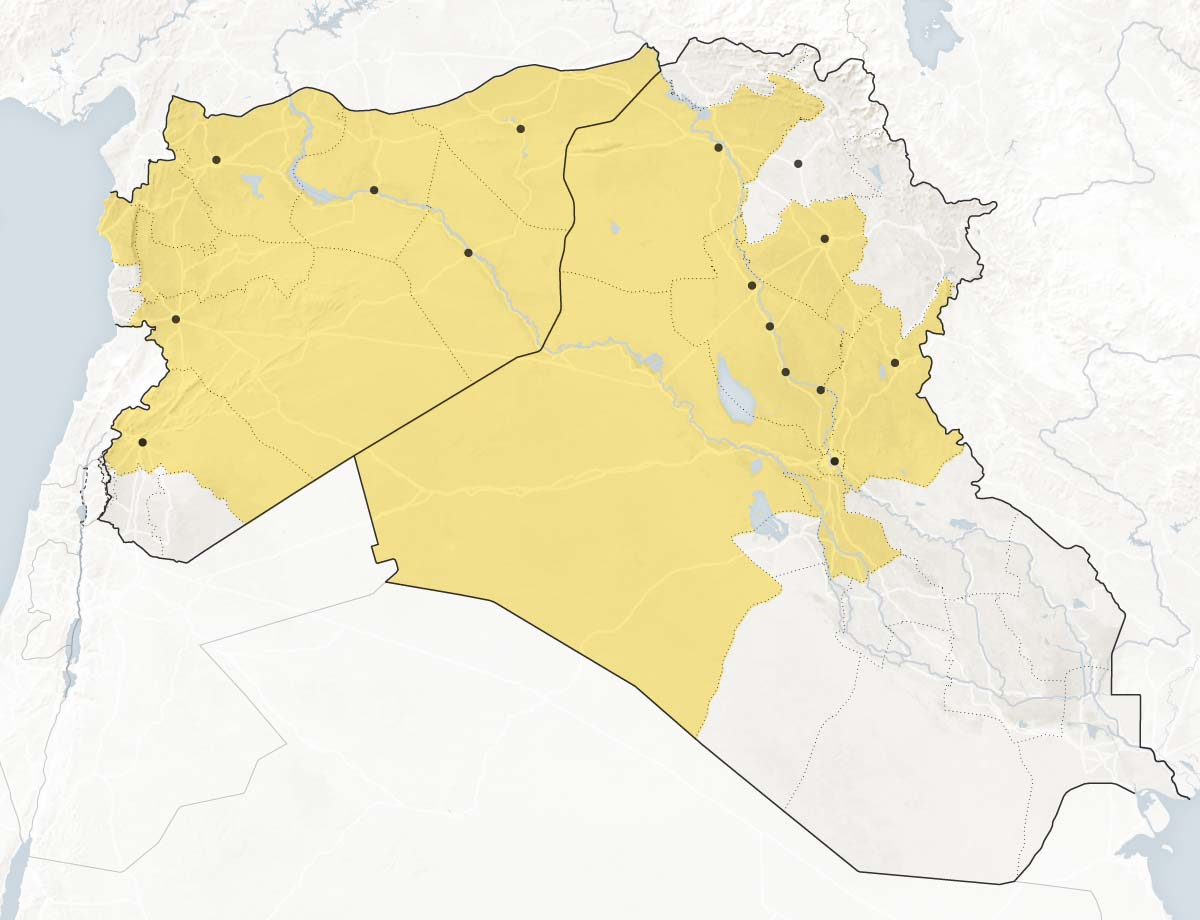
\includegraphics[trim = 0cm 0cm 0cm 0cm, clip,scale=0.3]{./figures/current2.png}
   \caption{My Caption \cite{Lewis2014}}
     \label{fig:current2}
\end{figure}


\subsubsection{??????  Needs a reference   ???????}

\begin{figure}[H]
 \centering
 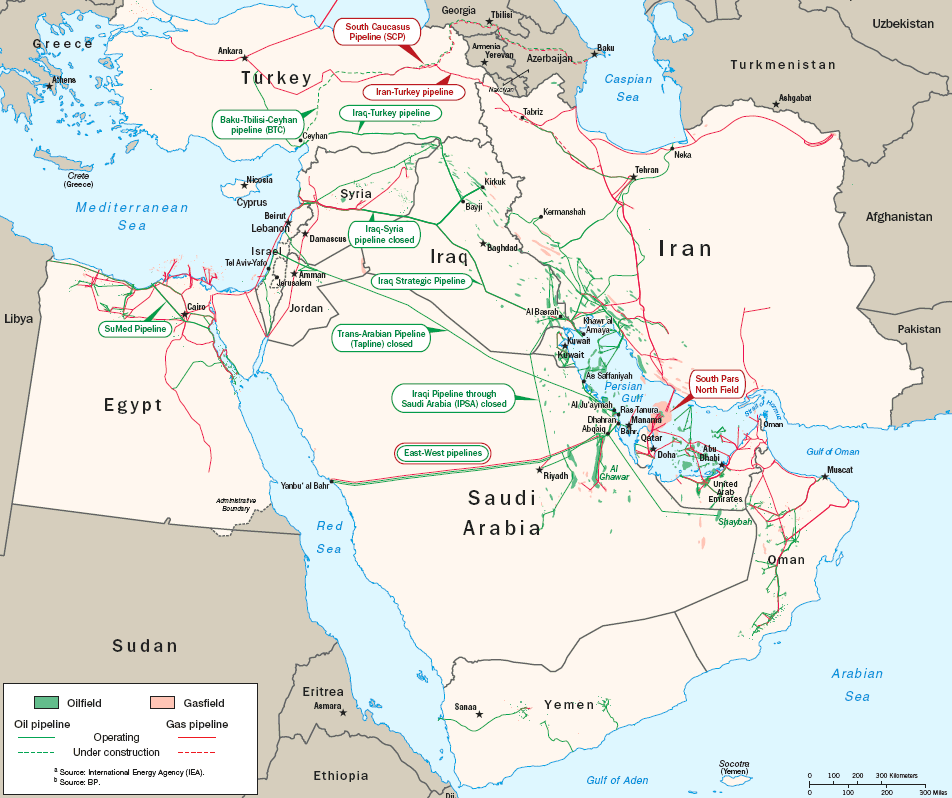
\includegraphics[trim = 0cm 0cm 0cm 0cm, clip,scale=0.4]{./figures/oil_reserves.png}
   \caption{Oil Reserves and Ground Transportation Routes}
     \label{fig:oil_reserves}
\end{figure}


\subsubsection{??????  Needs a reference   ???????}

\begin{figure}[H]
 \centering
 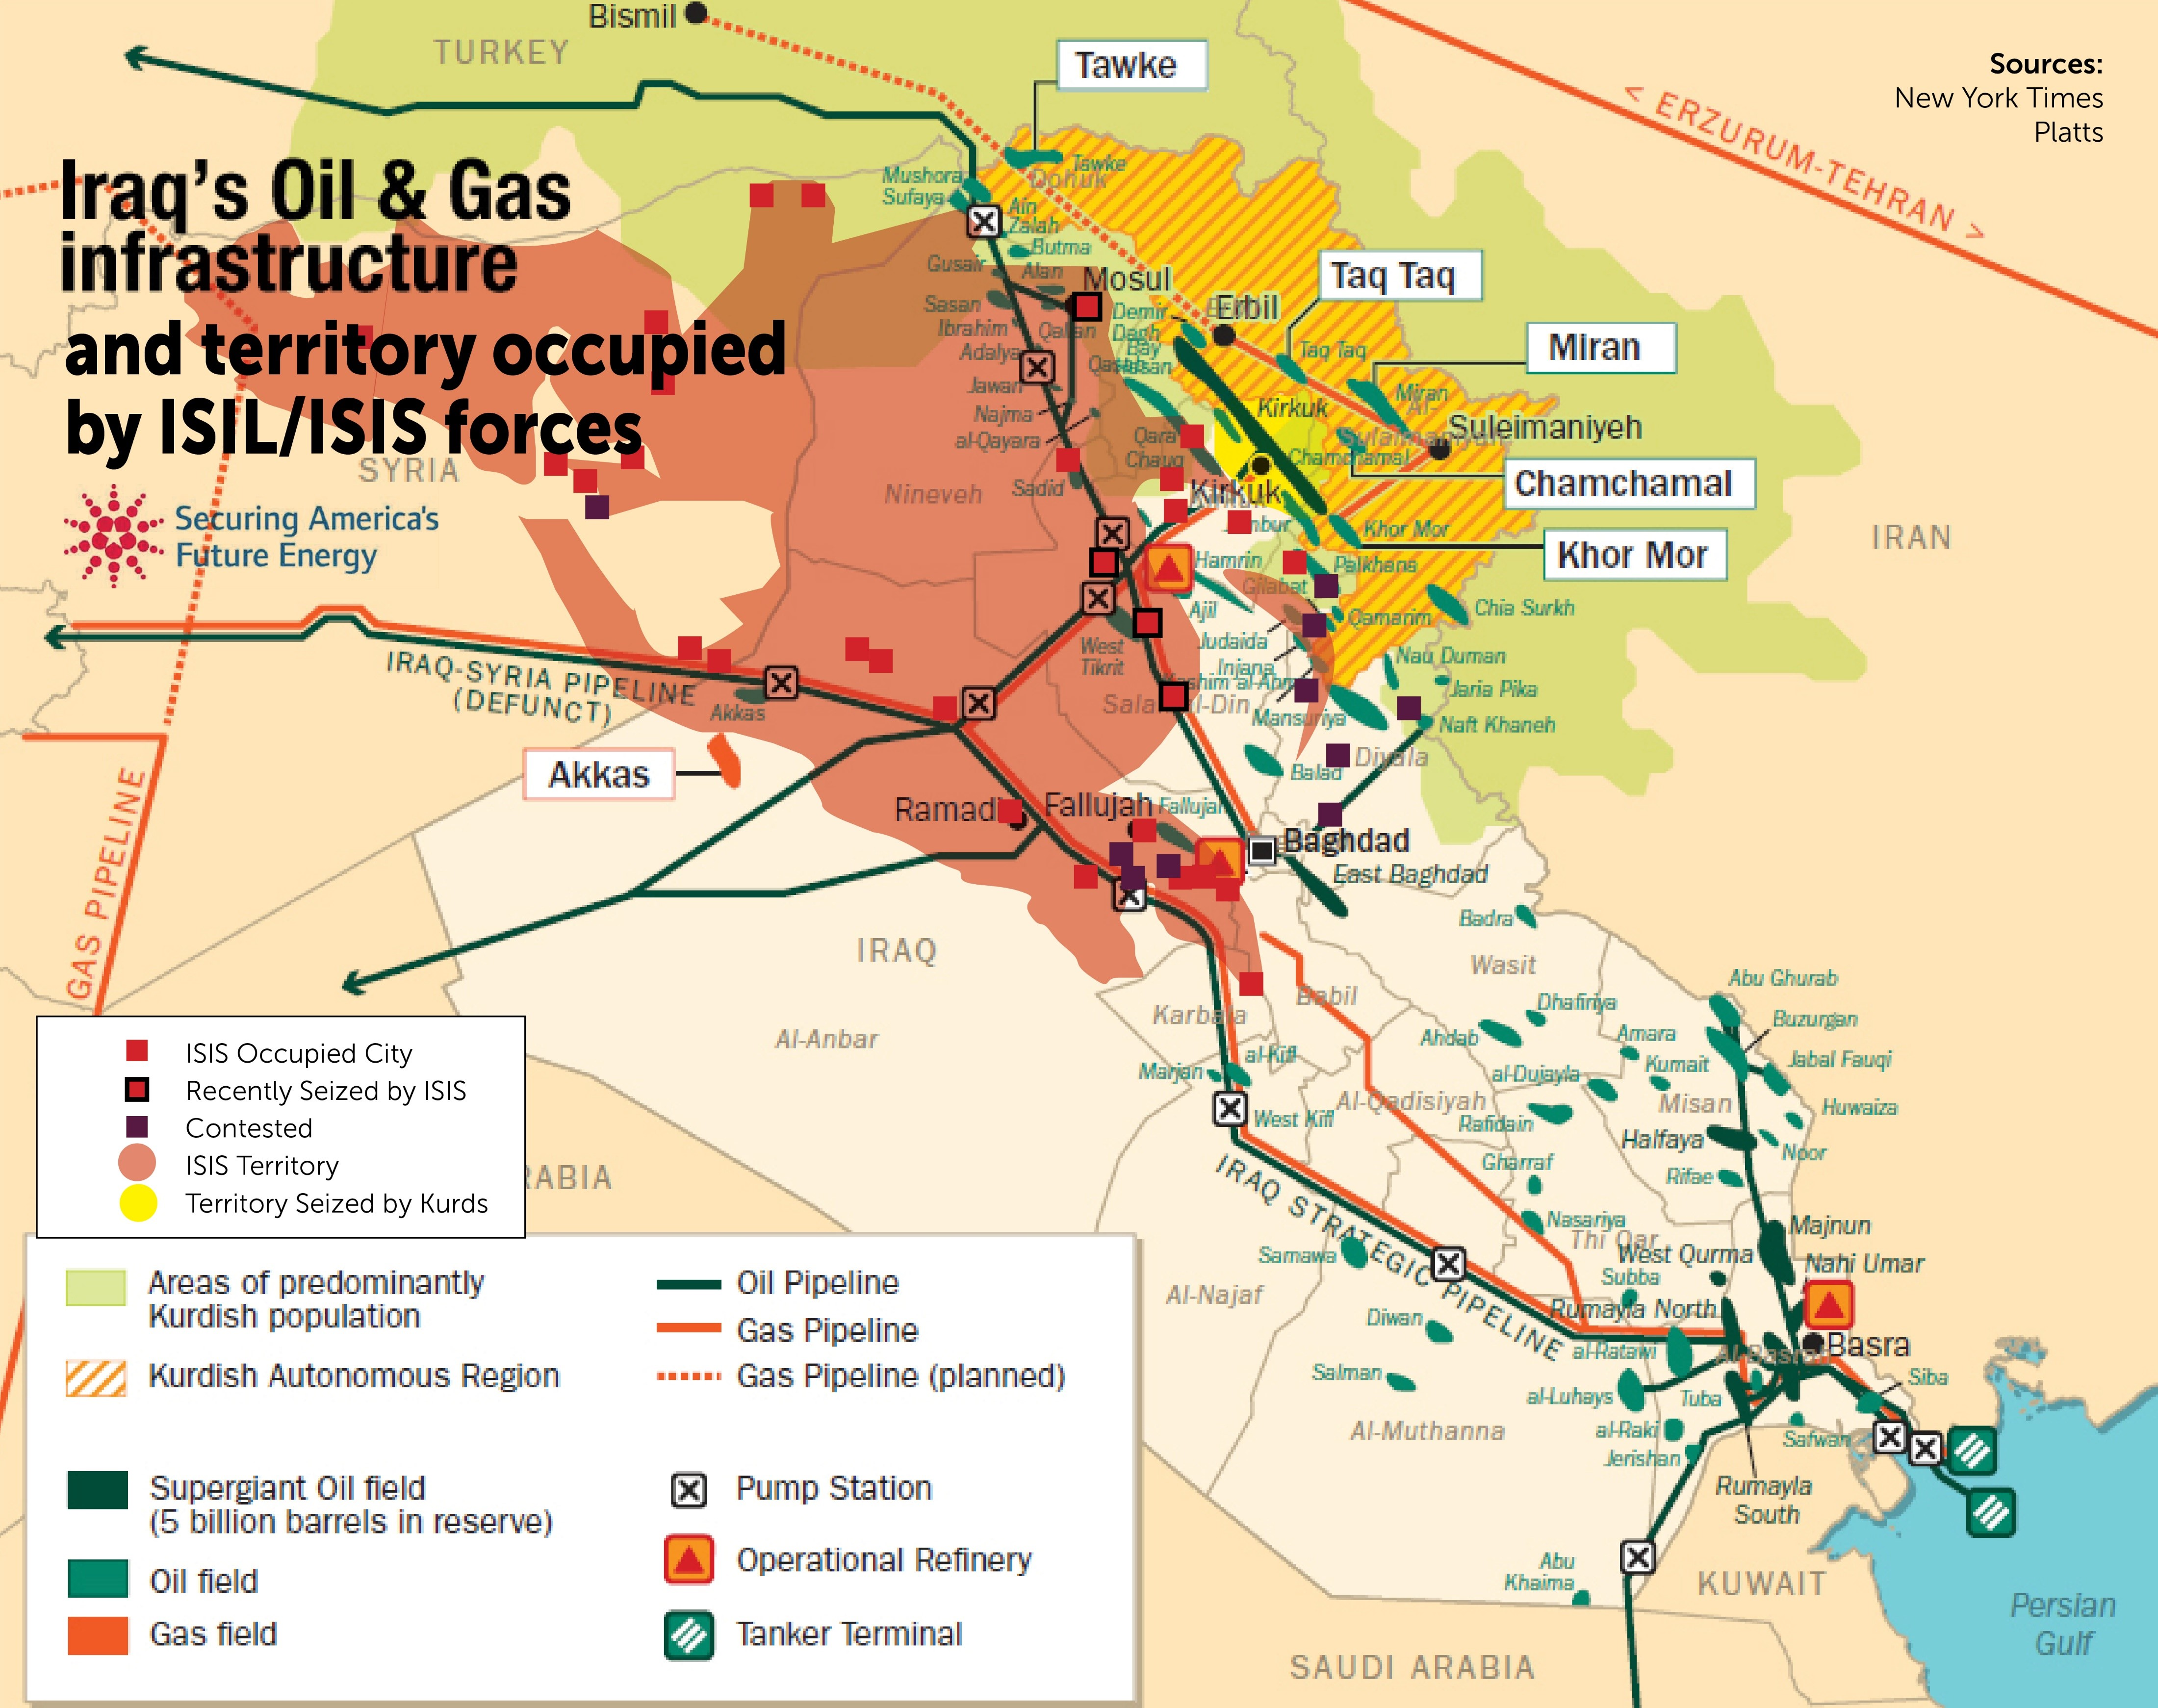
\includegraphics[trim = 0cm 0cm 0cm 0cm, clip,scale=0.3]{./figures/oil_infrastructure.jpg}
   \caption{My caption}
     \label{fig:oil_infrastructure}
\end{figure}


\subsubsection{??????  Needs a reference   ???????}

\begin{figure}[H]
 \centering
 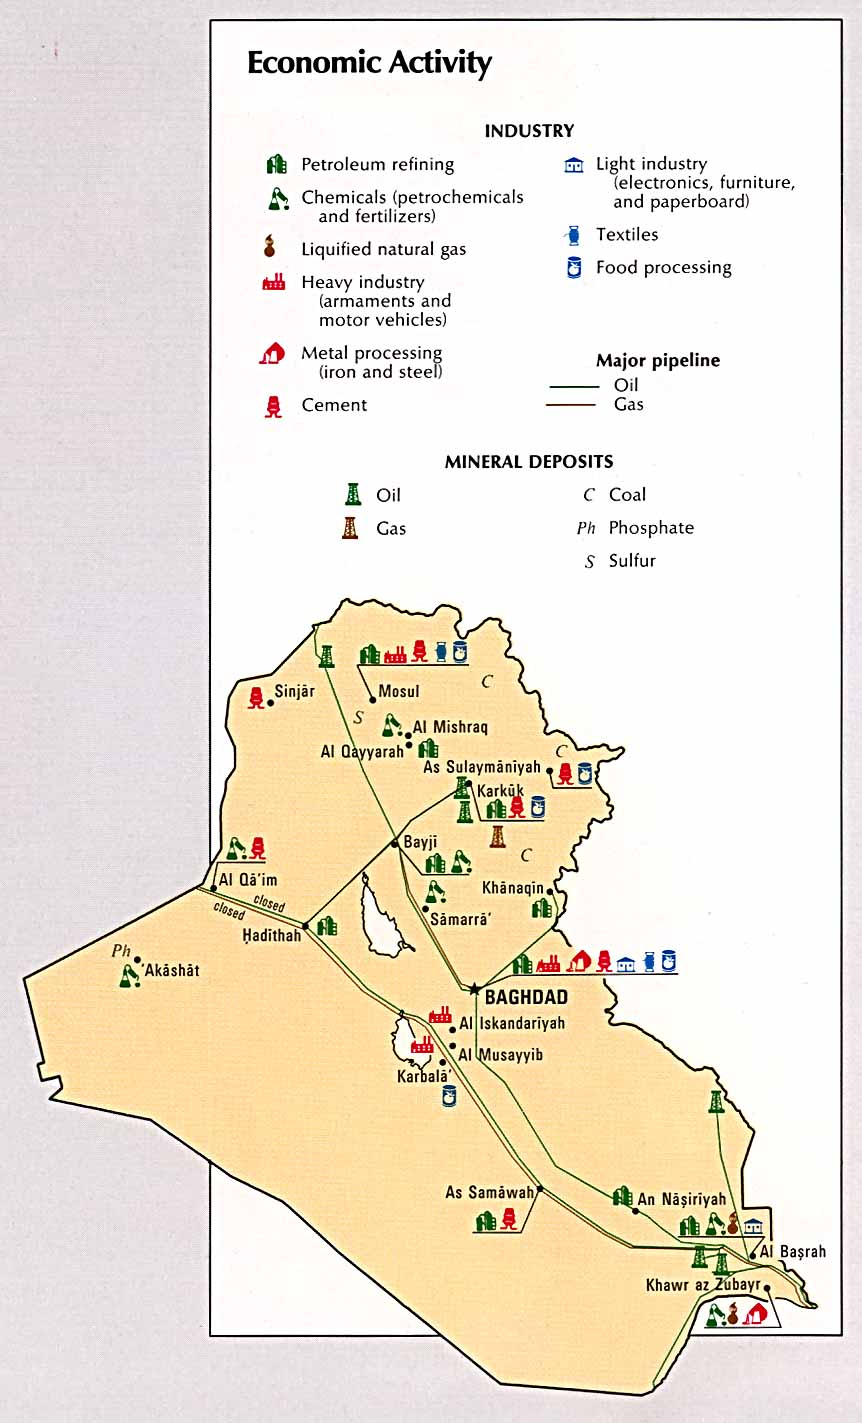
\includegraphics[trim = 0cm 0cm 0cm 0cm, clip,scale=.7]{./figures/minerals.jpg}
   \caption{Mineral Deposits and Industry in Iraq}
     \label{fig:minerals}
\end{figure}



\subsubsection{??????  Needs a reference   ???????}

\begin{figure}[H]
 \centering
 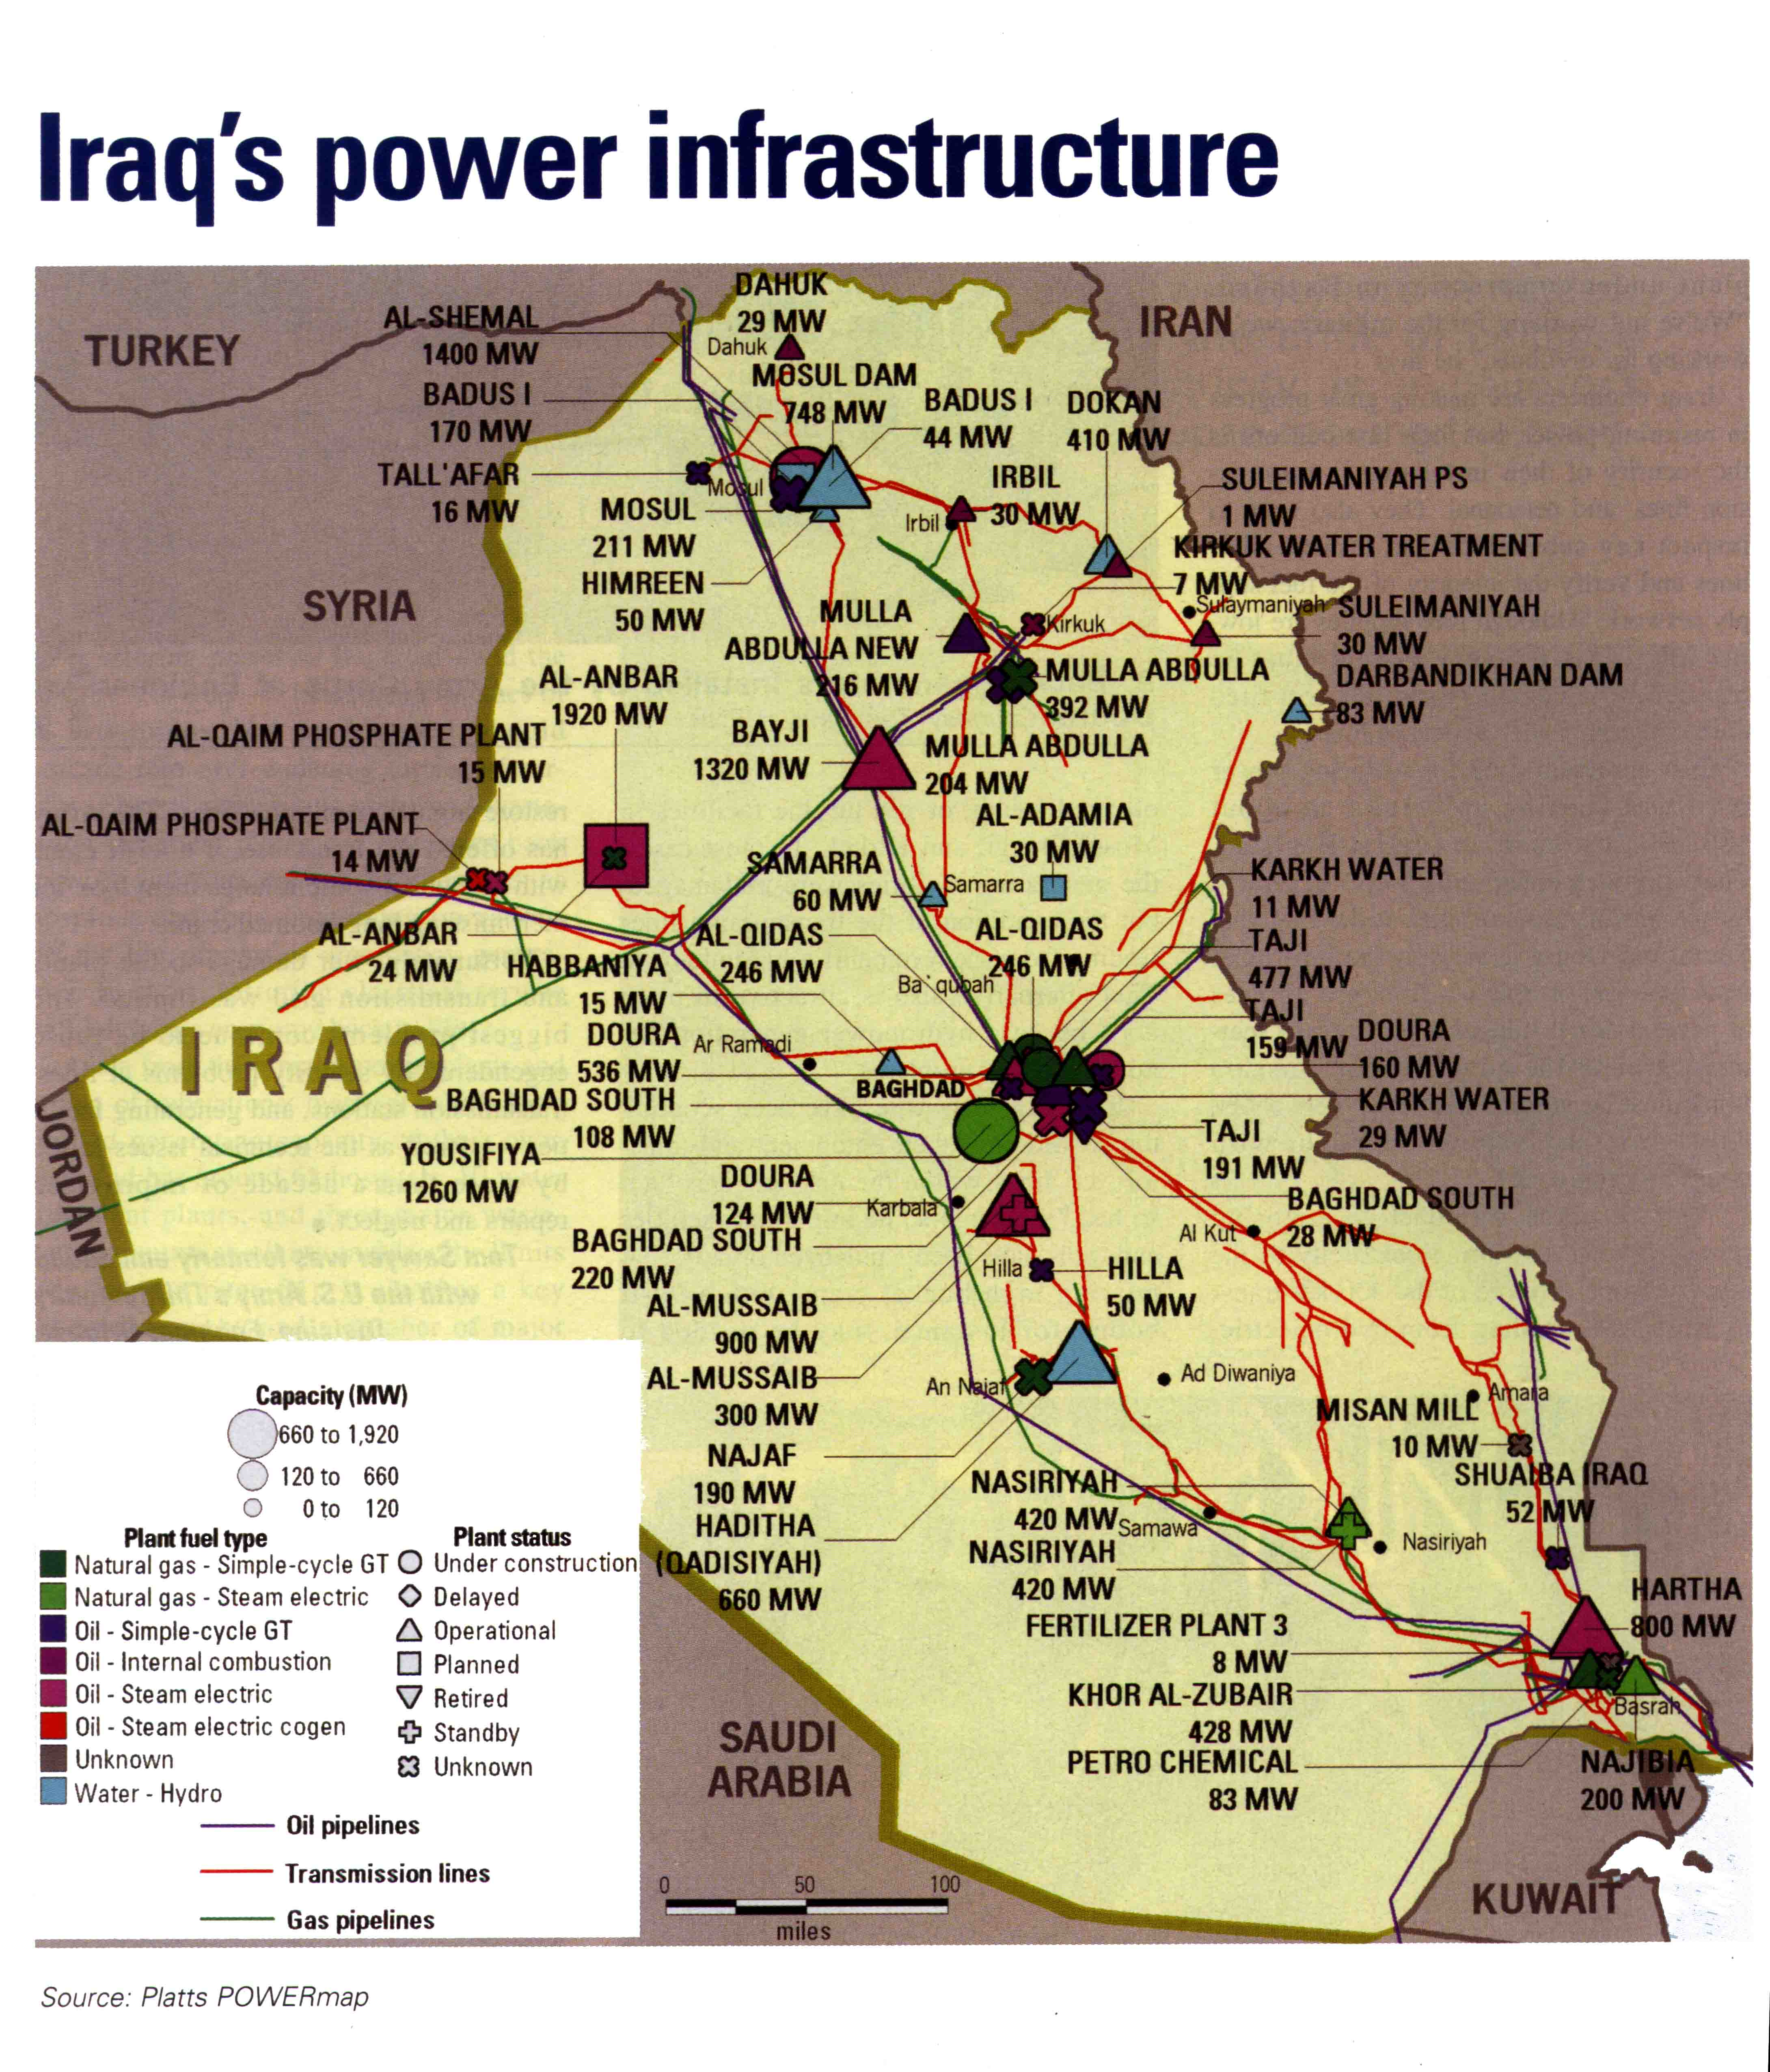
\includegraphics[trim = 0cm 0cm 0cm 0cm, clip,scale=.6]{./figures/elec_grid.jpg}
   \caption{Iraqi Electricity Grid}
     \label{fig:elec_grid}
\end{figure}



Image courtesy of Global Energy Network Institute



\subsubsection{??????  Needs a reference   ???????}

\begin{figure}[H]
 \centering
 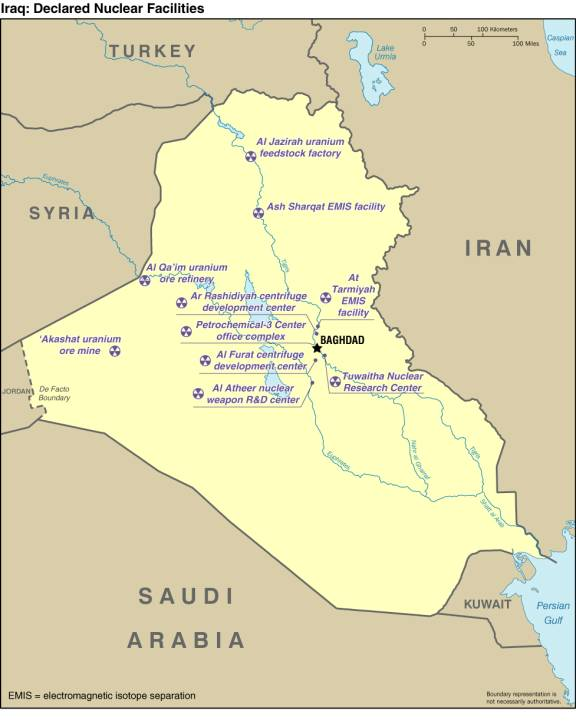
\includegraphics[trim = 0cm 0cm 0cm 0cm, clip,scale=.6]{./figures/nuke_facilities.jpg}
   \caption{Iraq Declared Nuclear Facilities (as of 2002)}
     \label{fig:nuke_facilities}
\end{figure}





Image courtesy of Federation of American Scientist Report



\subsubsection{??????  Needs a reference   ???????}

\begin{figure}[H]
 \centering
 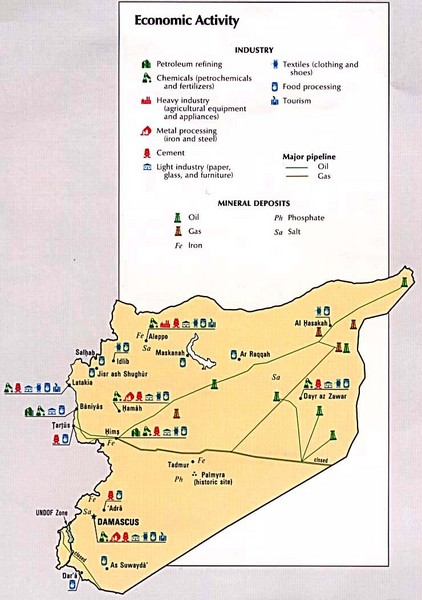
\includegraphics[trim = 0cm 0cm 0cm 0cm, clip,scale=1]{./figures/syria_minerals.jpg}
   \caption{Mineral Deposits and Industry in Syria}
     \label{fig:syria_minerals}
\end{figure}




\subsubsection{??????  Needs a reference   ???????}

\begin{figure}[H]
 \centering
 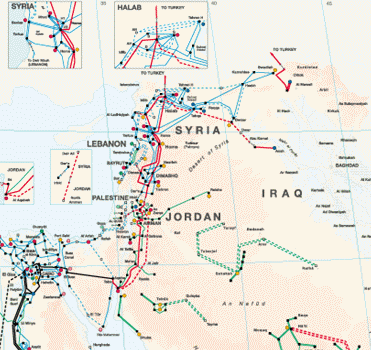
\includegraphics[trim = 0cm 0cm 0cm 0cm, clip,scale=1]{./figures/syria_grid.png}
   \caption{Syrian Electricity Grid}
     \label{fig:syria_grid}
\end{figure}





Image courtesy of Global Energy Network Institute




\subsubsection{??????  Needs a reference   ???????}

\begin{figure}[H]
 \centering
 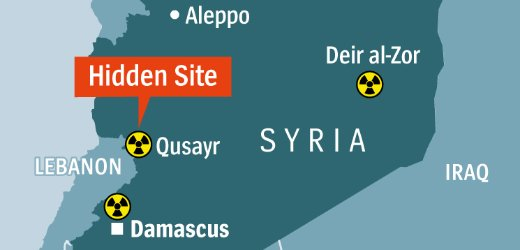
\includegraphics[trim = 0cm 0cm 0cm 0cm, clip,scale=0.7]{./figures/syria_nuke_facilities.jpg}
   \caption{Syrian sites of possible nuclear facilities}
     \label{fig:syria_nuke_facilities}
\end{figure}




Picture courtesy of Der Spiegel






\subsection{Counteract ISIL's draw to foreign fighters.}

ISIL has shown itself prolific at recruiting foreign fighters, and the U.S. must try to stem this flow in its entirety, but also to prevent nuclear scientists from joining ISIL's causes. 

There are two keys reasons why nuclear scientists may choose to aid ISIL in the procurement of a nuclear device:

\begin{enumerate}
  \item Monetary reasons, which would be a result of lack of employment
  \item Ideological reasons
\end{enumerate}


The most effective way to deal with the first possibility is to ensure that nuclear scientists have steady employment and research opportunities. This was the approach used by the Clinton administration to deal with the threat from the former Soviet Union in the wake of the late 1990's Russian financial crises. In the Congressional Research Service's report for congress, Amy Woolf and Curt Tarnoff described the steps taken in 2000:

\subsubsection{????????  Need a more concrete reference for this block quote   ?????????}


\blockquote{The Clinton Administration has responded by proposing the Expanded Threat Reduction (ETR) Initiative. According to the President's budget for FY2000, funding for threat reduction programs would increase from \$742 million in FY1999 to \$1 billion in FY2000. Over the next five years, planned spending would increase from \$2.7 billion to \$4.5 billion. The added funds would not only augment ongoing programs to secure nuclear, chemical, and biological weapons and materials, it would also expand programs that focus on keeping scientists and engineers away from rogue nations. Specifically, in FY2000, funding for DOD programs and DOE programs, both authorized in the DOD authorization and appropriated in the DOD and Energy and Water appropriations bills respectively, would increase a small amount over FY1999 levels (\$35 million and \$28 million respectively), while State Department programs, funded in the Foreign Operations appropriations bill, would increase by nearly \$200 million from FY1999 to FY2000. In the long term, \$1.1 billion of the \$1.8 billion that the Initiative adds to planned threat reduction programs between FY2000 and FY2004 would go to DOD's CTR program. Another \$500 million of the proposed addition would go to DOE programs, and the State Department would receive the remaining \$200 million in added funds.

\subsubsection{???????? not sure the first paragraph of this quote is necessary, unless your saying that we should spend comparable amounts of money now. also, you can probably just integrate the points of the second paragraph into your own paragraph, no real need to pull it out as a block quote  ?????????} 

The State Department manages several programs that offer NIS scientists employment and research opportunities, so that they will be less likely to sell their knowledge to rogue nations. The International Science and Technology Center (ISTC) in Moscow and the Science and Technology Center in Ukraine (STCU), multilateral programs supported by the EU, Japan, and others, fund research in such areas as nuclear reactor safety, medicine, civil aviation, and energy production. A \enquote{Partners Program} links NIS scientists with contributing U.S. private sector companies, such as General Electric and Lockheed Martin, and academic institutes to assist their own R\&D efforts. The Civilian Research and Development Foundation (CRDF) is a private, non-profit foundation, originally funded by matching grants from DOD and George Soros. It supports U.S. collaboration and exchanges with former NIS defense scientists on civilian basic and applied research, and supports projects with commercial applications. The State Department also implements a pilot project for biological weapons scientists to \enquote{redirect} their expertise toward commercial endeavors. Among other activities, it has established a collaborative program between the Department of Agriculture's Agricultural Research Service and Russian scientists on agriculture research, and between the Department of Health and Human Services' Centers for Disease Control, National Institutes of Health, and Food and Drug Administration and Russian biomedical scientists to conduct research on infectious diseases. }

We should recommend that DoS is continuing with these initiatives, and if possible increase funding for employment and research opportunities for nuclear scientists. The second threat – that nuclear scientists will aid ISIL for ideological reasons – is of lesser probability, \subsubsection{???????? source?? ?????????} but more difficult to deal with. The steps that must be taken include a number of initiative to degrade ISIL's image as a leader in the Muslim world, which is part of the larger fight against ISIL as a whole, and is not included in depth in this report. 

\subsection{Domestic Portal and Border Monitoring}

\subsubsection{??????  Needs content proofing ???????}


As with any foreign terrorist threat, it is imperative to assess the United States' domestic capabilities for the detection and interception of weapons and materials that pose a significant risk to American security. In the context of this section, we specifically consider nuclear weapons and materials that have the potential to be detonated domestically after being smuggled past American borders. We examine current and past efforts and capabilities to prevent such weapons from entering the United States undetected, as well as the possibilities for the development and implementation of better detection technologies. 

Two of the relevant governmental organizations regulating domestic borders and security are the Federal Bureau of Investigation (FBI) and the Department of Homeland Security (DHS). Together, these organizations are responsible for the security of the United States against both domestic and foreign threats. They coordinate intelligence gathering as well as threat-response and eventually coordinate with the justice system. With these goals in mind, a significant portion of their work deals with the monitoring of borders. The Department of Homeland Security alone commands more than 180,000 personnel, operating such sub-groups as the U.S. Coast Guard, U.S. Customs and Border Protection (CBP), and the Immigration and Customs Enforcement (ICE) \cite{Robb2005}. One of the most relevant DHS sub-groups is the Domestic Nuclear Detection Office (DNDO). The DNDO is responsible for the development and deployment of radiation and detection equipment to assist any other federal agency, including the other DHS sub-organizations and the FBI \cite{UnitedStatesGovernmentAccountabilityOffice2013}. 

The aforementioned government agencies have correctly addressed border and seaport monitoring as a location of high potential for the interception and detention of nuclear weapons and materials. In 2005, the CBP in collaboration with the American Association of Port Authorities (AAPA) had already begun deployment of a large network of Radiation Portal Monitors (RPMs) with a comprehensive plan for 100\% screening of the locations seen in \autoref{fig:RPM_map} \cite{Simmons2005}. 


\begin{figure}[h]
 \centering
 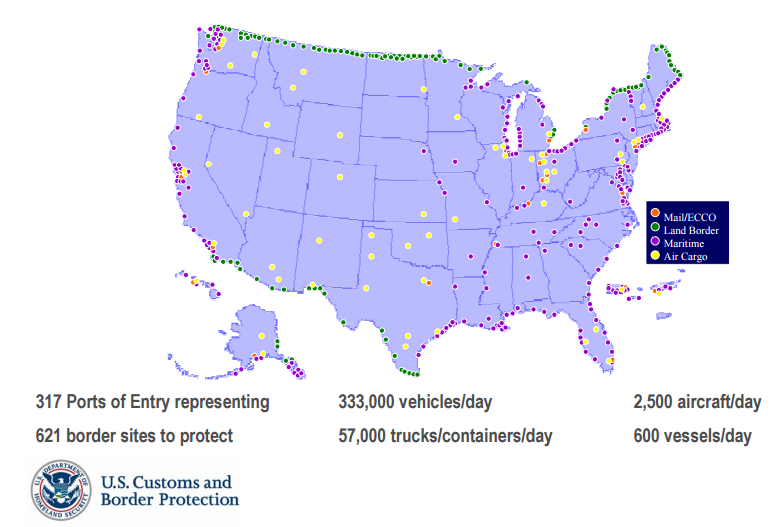
\includegraphics[trim = 0cm 0cm 0cm 0cm, clip,scale=0.55]{./figures/RPM_map.png}
   \caption{CBP plan for RPM deployment \cite{Simmons2005}.}
     \label{fig:RPM_map}
\end{figure}


The CPB/AAPA RPM plan outlines a phased implementation targeting locations on a priority basis around the U.S. The plan additionally details a technology collaboration with the Pacific Northwest National Lab (PNNL), who was responsible for the development of cutting-edge, harmless and passive detection systems (illustrated in \autoref{fig:RPM_designs}). In 2005, RPM systems had already been deployed at 14 terminals, with another 18 in construction and 27 in final design \cite{Simmons2005}.

\begin{figure}
        \centering
        \begin{subfigure}[b]{0.3\textwidth}
                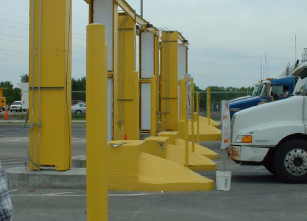
\includegraphics[width=\textwidth,scale=1]{./figures/fixed_vehicle.png}
                \caption{Fixed  vehicle monitor.}
                \label{fig:fixed_vehicle}
        \end{subfigure}%
        ~ %add desired spacing between images, e. g. ~, \quad, \qquad, \hfill etc.
          %(or a blank line to force the subfigure onto a new line)
        \begin{subfigure}[b]{0.3\textwidth}
                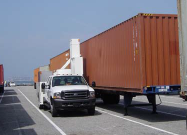
\includegraphics[width=\textwidth,scale=1]{./figures/mobile_cargo.png}
                \caption{Mobile cargo monitor.}
                \label{fig:mobile_cargo}
        \end{subfigure}
        ~ %add desired spacing between images, e. g. ~, \quad, \qquad, \hfill etc.
          %(or a blank line to force the subfigure onto a new line)
        \begin{subfigure}[b]{0.3\textwidth}
                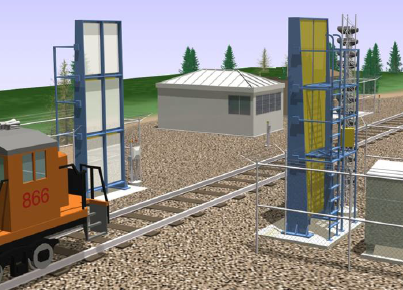
\includegraphics[width=\textwidth,scale=1]{./figures/perm_train.png}
                \caption{Permanent train monitor.}
                \label{fig:perm_train}
        \end{subfigure}
        \caption{RPM designs and illustrations \cite{Simmons2005}.}\label{fig:RPM_designs}
\end{figure}
  


Eight years after the initial development of the RPM plan, the Office of the Inspector General published a report documenting the progress made in the RPM development specifically at seaports \cite{DepartmentofHomelandSecurityDHS2013}. The document reports 444 active RPMs screening 99\% of inbound containerized cargo at large seaports, with the other 1\% of cargo entering low-volume seaports (this 1\% presumably not monitored). 


One point of concern outlined in the report is that many RPM devices (up to 10\% at a large port) were no longer being used. Further, given the limited use of funds for the DNDO and CBP, no plans (as of the report in 2013) were put in place to ensure continued use of RPM technology. Recommendations were generated in the report to develop an organization to ensure the continued and efficient use of RPMs at seaports. 


Development of advanced RPM technologies (meant to replace the old devices) has been continued in recent years, although not necessarily with great success. In 2013, the Government Accountability Office released a report outlining the technical failure of the development of Advanced Spectroscopic Portal Monitors (ASPs) \cite{UnitedStatesGovernmentAccountabilityOffice2013}. Lessons were outlined and documented from the failed attempt at replacement RPMs, but years after the final technology tests. Overall, the entire process was quite cumbersome and ineffective. 

In order for the U.S. to be effectively guarded against potential nuclear terrorist threats from cunning organizations such as ISIL, a streamlined, more efficient approach must be taken to portal and border monitoring. True, the initial development and deployment of RPM technology seems to have been fairly effective based on publicly - available reports \cite{Simmons2005,DepartmentofHomelandSecurityDHS2013}. The caveat to these programs is their reported deterioration over a decade of dormancy. 

\subsubsection{?????????  Add in cross-reference to below paragraph, once Tech Appendix is made  ??????????? }

This document suggests the aggressive continued advancement of such programs. The continued development of new technologies, as outlined in \autoref{}, must be exploited for every feasible advancement leading to total success in national security. This document suggests a priority-phased plan outlining a strong technological collaboration with government labs, similar to the plan put forth in 2005, in order to develop and deploy the next generation of RPMs \cite{Simmons2005}. Such a plan would be managed by the DNDO and executed by the CPB and AAPA. This plan, however, can only be effective given the successfully executed deployment of any resulting technology. Technological failures such as the ASP development program are acceptable so long as a workable solution is subsequently achieved. 




\subsection{Proliferation of RDD materials}

Interception (proliferation)
 
\subsubsection{Fission Weapons}

ISIL could attempt to purchase or steal a nuclear weapon, and so the nations which maintain a stockpile of nuclear weapons must remain under scrutiny. Nations of the highest interest that have nuclear weapons are Pakistan, North Korea, India, Turkey, Israel, and Russia. Israel has not been confirmed to have nuclear weapons, but it is widely believed that it has nuclear capabilities. Turkey is a NATO nuclear weapon sharing state and has U.S. tactical nuclear weapons stationed within its borders. However, it is unlikely that ISIL would be able to steal a nuclear weapon from either of these states, as those in Turkey are under U.S. protection and Israel has proven adept at hiding their arsenal. Of greatest concern is the possibility that any of these nuclear-capable states, North Korea in particular, would willingly sell a physics package to ISIL.

The purchasing of nuclear materials, while it could be done on a national level, is much more likely to occur through individuals. The only collection of nation confirmed information on incidents of illicit trafficking and other unauthorized activities involving nuclear and other radioactive material is called the ITDB \subsubsection{???????? what does this acronym stand for?  ?????????} and is maintained by the IAEA. As of 2006, over 1000 incidents of illicit trafficking and other unauthorized activities involving nuclear and other radioactive material has been reported to the IAEA with about 25\% specifically involving nuclear materials \cite{Iaea2007}. A majority of these cases involve highly enriched uranium (no plutonium). One such incident occurred in 1994 when an individual stole 2.972 kg of highly enriched uranium from a nuclear factory \cite{Iaea2007}. See \autoref{fig:seizures} for more information on the location and size of notable seizures. 

\begin{figure}[h]
 \centering
 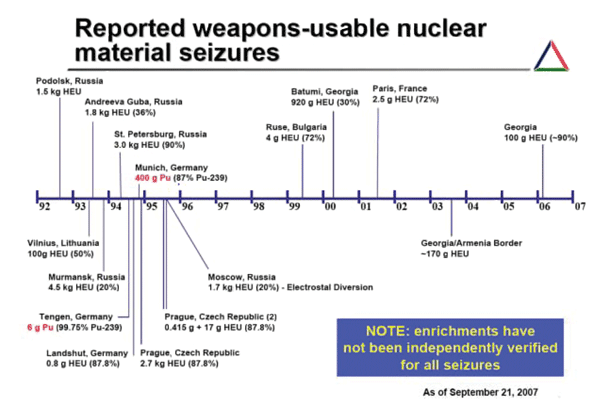
\includegraphics[trim = 0cm 0cm 0cm 0cm, clip,scale=0.7]{./figures/seizures.png}
   \caption{Location and time of global seizures of special nuclear materials \cite{Muller2007}.}
     \label{fig:seizures}
\end{figure}


Most of these instances are very small amounts (grams) but there have been several involving one to three kilograms. No individual case has been found with enough material to make a nuclear bomb, but multiple thefts could allow ISIL to accumulate enough special nuclear material to create a nuclear weapon. 

The non-proliferation treaty (NPT) assists with prevention of these nations selling or having their weapons stolen. The NPT has a multitude of safeguards in place, including accounting for the flow of materials in and out of nuclear facilities, physical security, and containment and surveillance.However, while the NPT's has been effective in preventing nations from using existing energy facilities to make off the books weapon grade materials (these would be easier to sell), Iran, Iraq, and North Korea were able to set up separate facilities for creating weapons grade material. While these facilities were set up without international knowledge, they were discovered in Iraq and North Korea rather quickly.


\subsubsection{RDD}
 Some of the materials required to build an RDD are naturally occurring elements that are naturally radioactive. Other components are solely available to radiological work sites such as reactor facilities, isotope production, research and universities, weapons production facilities, and other commercial and industrial facilities. 

The lands surrounding ISIL are vast, and currently a large majority are under militant occupation.  The probability that materials of this nature can move about the region is very high.  Paid courier services, as well as stolen armed and armored transportation vehicles  may assist in this endeavor.

\subsubsection{???????? Identify possible and likely sources of the top 10 RDD materials identified in section 2.2 that ISIL might purchase or steal. Also identify possible sources of these materials within territory that ISIL controls (such as hospitals and universities). Discuss any current export controls on these materials, and how they might inhibit the acquisition of significant quantities of materials. Discuss the orphan source program, or any other international institutions which regulate the creation and distribution of radioactive sources. (To be added by 4/19; possible add map of sources?) ?????????????} 
 
 \subsection{Flow of fission weapons/materials}

Merge with above subsection?


\subsection{Flow of non-nuclear but necessary technologies}

Flow of non-nuclear but necessary technologies (Sandia components)
Export control regimes

A significant concern identified earlier in this report is the possibility of a nuclear-capable state willingly selling a physics package to ISIL. The associated non-nuclear delivery technologies are also significant proliferation risks from states with the developed capabilities, if not more significant due to less oversight from international organizations and control regimes coupled with a higher degree of technology proliferation. Relevant delivery systems for WMD ISIL may consider include ICBMs, cruise missiles, and gravity bombs. 

There are more than thirty countries now capable of domestically producing ballistic or cruise missiles, including North Korea and to a lesser extent Iran \cite{U.S.CongressOfficeofTechnology1993}. Despite the increasing risk of proliferation of delivery systems for WMD, there is no binding international nonproliferation treaty that controls the spread of missiles or other delivery systems. There are two major examples of regimes that work to limit the proliferation of WMD delivery systems. The Missile Technology Control Regime is an informal and voluntary association of countries that work together to limit the proliferation of unmanned WMD delivery systems. The 2002 Hague Code of Conduct against Ballistic Missile Proliferation contains a set of general principles that its subscriber states pledge to follow. Neither of these sets of rules are binding, and neither include the states of most concern: North Korea, Pakistan, India, and Iran.

Cruise missiles, due to their simpler designs and lower costs, are more widely proliferated. Many cruise missile designs specifically avoid export controls specified by the Missile Technology Control Regime. The combination of \enquote{over-the-counter} technology, high probability of defense penetration in supersonic cruise missiles, and a relatively low barrier to technology development make cruise missiles ideal for initial acquisition followed by indigenous development and use \cite{OfficeoftheUnderSecretaryofDefenseforAcquisitionandTechnology1998}. 

The simplest delivery system is a combat fixed-wing aircraft coupled with a gravity bomb package. It is generally assumed most states seeking WMD already possess aircraft or can purchase them in international markets, and this assumption holds true for ISIL as well. Manned aircraft represent the most probable and delivery system for a WMD. 

The most probable path for ISIL to acquire a WMD delivery system would be to purchase or steal fixed-wing aircraft. This option is the easiest to achieve and most flexible, although the most vulnerable to disruption mid-delivery. However, a second and possibly more realistic use of nuclear materials by ISIL would be a RDD \cite{D.Esfandiary2014}. Delivery systems for RDDs are not limited to the traditional set discussed above, and small yield or compact designs can even be hand-carried to the target. The use of RDDs does not require the delivery systems discussed and nullifies arguments for delivery systems control. 










\chapter{Notes on response to successful weapons development}

Up to this point, the main focus of this policy has been the prevention of ISIL from developing, stealing, or buying a nuclear weapon or RDD.  However, it is necessary to develop a contingency in the unlikely event of failure in which ISIL obtains a weapon.  Unfortunately, the U.S. cannot use the same nuclear strategies it has in the past to deal with a nuclear ISIL.  The main focus of U.S. nuclear policy since the collapse of the Soviet Union has been non-proliferation.  There has not been as strong of a focus on deterring attacks from an adversary that already has nuclear capabilities \cite{Bracken2013}. However, even before the fall of the Soviet Union, deterrent strategies, such as counterforce, counter value, and mutually assured destruction, were tailored to deter an enemy state, not an extremist group.  Deterrence can only happen if the adversarial group/state thinks that the punishment received from the U.S. will outweigh the benefits of detonating a nuclear weapon \cite{kaplan1991wizards}.  It is unlikely that the U.S. will ever be able to make a threat that can deter ISIL.  Unlike the Soviet Union and other nuclear states, ISIL is made up entirely of militants who will die in defense of their religion and their caliph.  Death is not something that members of ISIL, or any other terrorist group, fear; it is something they celebrate.  They believe they will be rewarded in the next life for what actions on earth.  Even the threat of bombing by the U.S. and death will not deter them.  If they have reached the point of weapon acquisition, they have already ignored the United States' threats of massive retaliation and will likely continue to ignore any future threats.  For this reason, deterrence will be ineffective if ISIL acquires a bomb, so the U.S. must focus on other methods of stopping ISIL from detonating the weapon \cite{Sanderson2015}.

Once ISIL has a weapon, the next steps for them will be to develop a method of delivery, pick a target, and deploy and detonate the bomb.  If possible, the first priority of the U.S. should be to locate where ISIL is storing the bomb and destroy it using drone strikes.  However, it is highly improbable that the exact location of the bomb will be known or found using current detection technologies.  Even if it is found, it might be stored underground where drone strikes would not reach it.  Therefore, the more practical strategy for the U.S. will be to try to stop ISIL at each of the previously mentioned steps.   First, the U.S. will need to determine what delivery methods are possible for ISIL.  The U.S. can prevent ISIL from acquiring the necessary components to build more complex delivery system and slow down movement of the bomb.  Then, the U.S. can make predictions about the group's targets based on geographical location from ISIL and try to intercept the bomb before it reaches the target.  If all of that fails and the weapon is deployed, all the U.S. can do is to help minimize the damage.  Then, the U.S. and IAEA must be prepared to collect nuclear forensic data after the detonation in order to acquire data to prevent the construction and deployment of a second bomb.

The first step the U.S. can take after bomb acquisition by ISIL is to cut them off at their delivery method.  Generally, for nuclear powers, delivery methods are described by the nuclear triad: ground based missiles, such as ICBMs, strategic air bombers, and submarine-launched missiles.  However, as North Korea has shown, ground based missiles are not easily implemented.  It is highly unlikely that ISIL will be able to construct a long-range missile that can carry a nuclear weapon or a submarine capable of launching it.  North Korea has spent years trying to build ballistic missiles capable of delivering nuclear weapons over long ranges, and it is still questionable if they are capable of medium range distances \cite{Gladstone2015}.  It is also highly unlikely that any country will sell long-range missiles to ISIL.  As mentioned in \autoref{sec:global_rels} (\enquote{Global Relationships}), even though some nations may sell weapons to ISIL, it is still a low probability.  Also, none of these countries have ICBMs. North Korea and Pakistan do have short-range and some medium-range missiles \cite{Gladstone2015,NuclearThreatInitiative2014}.  Though, it is unlikely that these would be sold to ISIL, these countries should be heavily monitored in the event of bomb acquisition.  Submarine capabilities seem highly unlikely as well since they are more difficult to develop than land based missiles and the land that ISIL currently occupies is land locked.  The third part of the nuclear triad is long-range bombers.  However, few countries have long-range bombers and, of those countries, it is highly improbable that any of them would sell or give ISIL a bomber.  Therefore, the most likely method of delivery would be to ship or carry the bomb to the target depending on the location. 

The next step the U.S. can take is to predict the targets and intercept the bomb in transit to those targets.  It is unlikely that ISIL would use a nuclear weapon or RDD on cities in Syria or Iraq that they do not occupy since that would make the city and their resources unusable to them.  The fallout afterwards would also be close enough to hurt them as well.  It is more likely they will attack one of the other 61 countries in the Anti-ISIL Coalition \cite{Wordsworth2015}.  As mentioned earlier in this policy, it can be assumed that ISIL will follow a counter value strategy versus counterforce.  They are more likely to attack one of the population centers in one of these countries.  A major U.S. city would initially seem a primary target, however, due to the geographical distance from ISIL, it seems unlikely.  Since missile delivery is highly improbable, it would have to be shipped to the U.S..  However, there is no direct shipment method from ISIL to the U.S..  So, the bomb would be shipped through multiple ports and pass through multiple nuclear detector systems before reaching a U.S. port.  However, this possibility should not be ignored.  For this reason, if it is even suspected that ISIL has acquired a nuclear weapon, security at all U.S. ports should be increased.  Portal detectors should be used at all major ports and border crossings and at as many smaller ports as possible.  There is also the possibility of the attack of European countries.   However, as with the U.S., it is unlikely that ISIL will be able to ship it directly to any of the countries in Europe without it being detected.  However, another reason that European countries are not likely targets is due to the ideology behind ISIL.  ISIL's main targets are currently other Muslims who do not hold their extremist beliefs.  They are slightly more tolerant of Christians and Jews than \enquote{apostate} Muslims. \cite{Wood2015}  ISIL is therefore more likely to attack another Muslim nation, especially one that is geographically close.  Due to their close proximity and involvement in the Anti-ISIL coalition, Saudi Arabia, Jordan, Turkey and Lebanon are likely targets.  Iran is also another likely target due to its large Shia population.  Due to U.S.-Iranian relations and U.S. sanctions on Iran, it is unlikely that the U.S. and Iran will be able to work together on stopping a bomb from crossing over the Iranian border.  However, for the other countries, the U.S. can assist in monitoring their borders and possibly supply these countries with more advanced nuclear detection equipment.  With the U.S. and other countries in the Anti-ISIL Coalition focusing on these countries and their borders, it may be possible to stop the bomb from being delivered to its intended target.

If the bomb does reach its intended target, all the U.S. can do is try to minimize the damage and prevent a second detonation from happening.  If the U.S. or any other country is able to gather intelligence on where the bomb may be detonated but unable to find and disarm it, the best course of action is to try evacuating the area.  Depending on the country, the local government may or may not accept U.S. assistance in evacuating the area.  However, if the bomb was able to make it past all detection to its intended target, there is little chance that the U.S. or any other government will have any warning on where and when detonation will occur.  Once the bomb has detonated, the U.S. and the IAEA will need to work with the local government in order to collect samples and take the necessary measurements for post-detonation forensics.  Using this data, it may be possible to determine how ISIL obtained the weapon and to determine what signatures to look for in the future.  Hopefully, this information would prevent the acquisition and detonation of a second weapon.



\section{Weaponization to Target Selection}


Missing?




\chapter{???????   Things we still need to hit   ?????????}

\chapter{???????   Budget, cohesive implemented plan   ?????????}

\chapter{???????   Move bulk of info into appendices    ?????????}


ISIL taking over a major hospital/university - this is a major concern for chem/bio, I think, but not sure if there is a nuclear component. I know that for DoD, terrorist control of failed state capabilities (in the form of former/current facilities) for WMD purposes is a top concern.

Agency cooperation to manage and coordinate a crisis. This would include current actions to prepare to respond to a crisis, and might have lessons learned from Fukushima and Ebola in terms of inter-agency action. How do we utilize agencies and individuals without access to top secret information in the event of a loose nuke? There will be a lot of expertise that could help but intelligence community and white house won't want broad knowledge that ISIL may be getting close to nuclear device. 

This goes along with planning and preparing for a situation with a considerable lack of uncertainty. We're not just planning what to do, but planning structures that allow us to respond quickly to uncertainty. Looking for a lost nuke or lost nuclear material is like looking for a needle in a haystack. Since there is never a precise enough tool to find it, how do we shrink the haystack? How do we ensure we're leveraging collective knowledge of various agencies to zero in on it and verify if it's ISIL who has it. Even if we're keeping an eye on ISIL, are we developing capabilities for the event of a lost nuke (or whatever), to look and investigate, is there any way this thing is making its way to ISIL?

Utilizing Proliferation Security Initiative to track, interdict, and dispose of sensitive materials. There is some thinking on this in the Cooperative Threat Reduction.

There is significant competition within DoD over ISR (intelligence, surveillance, recognizance). How do we make sure the counterterrorism/WMD office gets enough of it to monitor nuclear materials in countries with ISIL sympathizers, and if we don't get it, what's the back up plan?

Broadly speaking, working this problem without assuming false precision. We don't want to assume we'll know exactly what ISIL has or where things are going, etc.

Going back and working with the maps that I sent you guys and trying to get all of that information about facilities and power grids and oil onto one or a couple maps. 

Any other big gaps that need attention.



\chapter{Conclusions and suggestions }

Waiting on Denia?





\appendix
\chapter[Appendix A: Glossary of Nuclear Terminology]{Glossary of Nuclear Terminology}  \label{app:glossary}



\textit{Note: All terminology is taken from the U.S. Nuclear Regulatory Commission  \cite{USNRC2015}.}

\textbf{Radioactive Decay:} The spontaneous transformation of one radioisotope into one or more different isotopes. The isotopes created may or may not also be radioactive. Radioactive decay may also be used to refer to the emission of a gamma ray or a conversion electron emission, which reduces the energy of the decaying isotope but does not change its identity. 

\textbf{Alpha Radiation:} The radioactive decay of a nuclide which results in the emission of a 4-Helium atom. Alpha radiation is sometimes followed by gamma emission. 

\textbf{Beta Radiation:} A radioactive decay of a nuclide which results in the emission of an electron and an electron antineutrino pair, or a positron and an electron neutrino pair. 

\textbf{Fusion:} A nuclear reaction in which atomic nuclei of low atomic number merge and become a heavier nucleus, thereby releasing energy. 

\textbf{Special Nuclear Material:} Plutonium, 233-Uranium, Uranium with enrichments of 233-Uranium or 235-Uranium.

\textbf{Gamma Radiation:} A radioactive decay which results in the emission of a high energy- short-wavelength, electromagnetic radiation emitted from within the nucleus of an atom. Gamma radiation often follows the emission of an alpha or beta particle, and always follows a fission event. 

\textbf{Electron Volt:} A unit of energy equivalent to the work required to accelerate an electron through a potential difference of 1 volt. 

\textbf{Fission:} The splitting of an atom, which releases energy. During fission, a heavy (large A) nucleus splits into two or three smaller nuclei and emits gamma rays and neutrons. 

\textbf{Nuclide:} A distinct nucleus, defined by the total number of neutrons and protons contained therein.  

\textbf{Fast Neutron:} A neutron with kinetic energy in excess of 1.5 MeV.

\textbf{Thermal Neutron:} A neutron which is in thermal equilibrium with its surroundings. 

\textbf{Fissile Material:} A nuclide that is capable of undergoing fission after capturing thermal neutrons.

\textbf{Fissionable Material:} A nuclide that is capable of undergoing fission after capturing a fast or thermal neutron.




% \appendix
\chapter[Appendix B: Intelligence Overview]{Intelligence Overview}  \label{app:intel}


\section{Intelligence Collection and Agency Responsibilities}

\subsection{?????????  Generally speaking, this Appendix could use some references ???????????}

Intelligence agencies gather information from physical and technical observations, conversations, searches, and human operations. These sources are grouped into Signals Intelligence (SIGINT), Imagery Intelligence (IMINT), Measurement and Signature Intelligence (MASINT), Human-Source Intelligence (HUMINT), Open-Source Intelligence (OSINT) and Geospatial Intelligence (GEOINT) \cite{Intelligen}. The National Security Agency (NSA) is responsible for SIGINT, and the NSA collects SIGINT using signal communications between people, machines, and combinations of both. National Geospatial-Intelligence Agency (NGA) is responsible for the collection of IMINT using visual collection methods including cameras, radars, lasers, etc. MASINT is technically and scientifically based intelligence on unique attributes of the desired target. MASINT is the part of the Defense Intelligence Agency (DIA) and can be used to recognize, locate, and describe the target through nuclear, seismic, acoustic, material, radio frequency, and optical sciences. The Department of State (DOS), CIA, Department of Defense (DOD), Federal Bureau of Investigation (FBI), and other agencies use HUMINT sources, more commonly known as spies, to gather data via photography, document transfer, information download, etc. in enemy territory. OSINT relies on publicly available information, and a large synthesis of OSINT is performed at Foreign Broadcast Information Service (FBIS) and the National Air and Space Intelligence Center (NASIC). GEOINT belongs to the NGA and is generally collected from satellites and reconnaissance aircraft. 

\subsection{Information Classification}

\subsection{??????? Add in Ref 10 below from Bushra  ???????}

The Information Security Oversight Office (ISOO) determines standards for information classification based on policy guidance from the National Security Council (NSC). ISOO has oversight of the extensive security characterization framework and the National Industrial Security Program. ISOO sets requirements for the original classification of information if the following apply: information should be classified by the classification authority; information is belongs to, controlled by, or is for the United States; information refers to one of the classification categories; classification authorities determines damage will be caused to national security from unsanctioned disclosure [10]. The classes of information classification believed to be effective \cite{Richelson2011}, [10].  The general classes of classification are:

10 Federal Register. "The President”, Part VII 75, 2010

\begin{itemize}
  \item Top secret: \enquote{exceptionally grave damage} to national security in case of disclosure.
  \item Secret: \enquote{serious damage} to national security in case of disclosure.
  \item Confidential: \enquote{damage} to national security in case of disclosure.
  \item Unclassified.
\end{itemize}

The information volume received from the all intelligence sources is astronomic. To facilitate the handling of this volume of information, assets are assigned based on the prioritization of the information. These are assigned as low, medium, and highly important:

\begin{itemize}
  \item \underline{Low (moderately serious)}: (e.g. planning to build weapon: enough time to plan actions and monitor progress).
  \item \underline{Medium (very serious)}: (e.g. weapon building in the process: actions should be taken ASAP).
  \item \underline{High (catastrophic)}: (e.g. weapon exists, ready to use: time is determining factor and actions should be taken immediately).
\end{itemize}

Combining these classification categories, a set of information and its sensitivity for the ISIL nuclear threat can be generated and is shown in \autoref{tab:separate_sec_level}.  

\subsubsection{?????? Be good to color code according to TS, S, C, or unclassified ???????}

% Please add the following required packages to your document preamble:
% \usepackage[table,xcdraw]{xcolor}
% If you use beamer only pass "xcolor=table" option, i.e. \documentclass[xcolor=table]{beamer}
\begin{table}[h]
\centering
\begin{tabular}{|c|l|c|c|c|}
\hline
\multicolumn{2}{|c|}{Information Category}           & \multicolumn{3}{c|}{Minimum Security Level}                                                 \\ \hline
\# & \multicolumn{1}{c|}{Information type}           & \cellcolor[HTML]{34FF34}LOW & \cellcolor[HTML]{FCFF2F}MEDIUM & \cellcolor[HTML]{FE0000}HIGH \\ \hline
1  & Information about weapon                        & \cellcolor[HTML]{34FF34}    & \cellcolor[HTML]{FCFF2F}X      & \cellcolor[HTML]{FE0000}     \\ \hline
2  & Information about weapon location               & \cellcolor[HTML]{34FF34}    & \cellcolor[HTML]{FCFF2F}       & \cellcolor[HTML]{FE0000}X    \\ \hline
3  & Information about target                        & \cellcolor[HTML]{34FF34}    & \cellcolor[HTML]{FCFF2F}       & \cellcolor[HTML]{FE0000}X    \\ \hline
4  & Information about persons related to the weapon & \cellcolor[HTML]{34FF34}    & \cellcolor[HTML]{FCFF2F}X      & \cellcolor[HTML]{FE0000}     \\ \hline
\end{tabular}
\caption{Separation of information by minimum security levels.}
\label{tab:separate_sec_level}
\end{table}

\subsection{International Intelligence Sharing}

Information sharing in the international IC is immensely more complicated than between internal U.S. agencies. The mere fact of declared opposition to ISIL is an insufficient basis for intelligence sharing alone.  Indeed, the U.S. various strained relationships with many allies in the fight against ISIL. It is assumed that information sharing on the ISIL issue would fall along lines consistent with historical cooperation levels. Cooperation levels can be divided into a simple system of three levels as shown in \autoref{tab:relation_table}.

\begin{table}[h]
\centering
\begin{tabular}{|c|l|}
\hline
Levels & \multicolumn{1}{c|}{Definition}                                                                                                             \\ \hline
1      & Historically and currently close relationship (Great Britain, France, Canada)                                                    \\ \hline
2      & \begin{tabular}[c]{@{}l@{}}Neither good nor bad relations or recent downturn in relations \\ For example: Germany as neutral [11] and Israel as recent downturn \cite{Goldberg2014}.\end{tabular} \\ \hline
3      & Historically and currently bad relationship (Russia, Jordan, Turkey, Egypt [10])                                                  \\ \hline
\end{tabular}
\caption{My caption}
\label{tab:relation_table}
\end{table}

\subsubsection{????????  This table needs a caption, reference  ???????}

A good example of informal multilateral agreement amongst level one countries is the United Kingdom – United States of America Agreement for cooperation in intelligence gaining between five English-speaking democracies: the United Kingdom, the United States, Canada, Australia and New Zealand \cite{Cox2012}. The collaboration began during World War II to track German and Russian signals and activities and endured for 70 years. The agreement enables the members to share intelligence facilities, avoid duplication, and combine strength. The U.S. and the UK have the most advanced technical abilities, biggest budgets, and are main players in the alliance. The U.S. operates intelligence centers in allied countries: one of the world's largest eavesdropping centers in Britain is run by NSA with hundreds of British employees from the Government Communications Headquarters (GCHQ); Pine Gap, a satellite tracking station in Australia, is run Partly run by the CIA, NSA, and U.S. National Reconnaissance Office (NRO). The agencies work side-by-side, allowing information flow quickly. The members of the alliance work with foreign intelligence to obtain local information without letting them into the alliance. Only U.S. intelligence officers can directly access the database; other country members have to show potential links to U.S. security threats for the information they request from the database. All members have benefited from the information sharing. The U.S. and UK prevented a major attack in 2006 designed to use liquid explosives to explode 10 airliners traveling from the UK to U.S. and Canadian destinations. 


\chapter[Appendix C: International Partnerships]{International Partnerships} \label{app:partners}

\section{Strategic Communication }

\subsection{????????  This appendix needs references  ???????}


Strategic communication became increasingly important with the advent of globalization and interconnectivity (borderless world) that led to rising threats from \enquote{transnational} issues. Security challenges no longer come in lone tangible entities, but instead are multi-polar and dispersed into gray areas where there are no clear cut answers, everything is connected, and second order effects must be accounted for. Strategic communication was developed to provide a framework to help solve the multi-polar problem that defines our current security environment.

Communications or exchanges of information (intelligence sharing) can be on the bilateral or multilateral level. Cooperating at the multilateral level diversifies sources of intelligence and increases the confidence in intelligence assessments. Multilateralism disproportionally benefits smaller countries with less bargaining power and resources, but working together with these countries can be effective in tackling issues of concern related to nuclear proliferation that may utilize black markets and networks that reside in their country. On the other hand, multilateral cooperation requires a complex system requiring organization and structure to ensure timely and accurate sharing of information. Additionally, the large number of participants can result in lower security of information thereby affecting the willingness of countries to share confidential and sensitive materials.

At the bilateral level, both sides can be more specific and develop tailored agreements. From a liberalism perspective, bilateralism can help larger states gain control over smaller states through a series of arrangements that maximize the influence of the larger state. However, bilateral cooperation can be more wasteful in time and effort as compared to a multilateral strategy. It can also be less reliable because no international norm is established creating compliance pressure, which can lead to compliance with the agreement becoming a bargaining chip to gain further concessions.

The U.S. sees merits in pursuing both multilateral and bilateral effort in international strategic communications. Most of the times, the U.S. tends to favored intense bilateralism over multilateralism to achieve its objectives. However, following World War II, multilateral initiatives in the area of nuclear non-proliferation and disarmament increased in significance.  This multilateral transition was marked by the creation of the United Nations (UN) in 1945.  The UN, and several subsequent agencies, are the current approach taken by the U.S. to address nuclear proliferation concerns.  

\subsection{Nuclear-Relevant Organizations }

The UN is the largest international organization that can take actions on the issues of security at a global level. Several divisions in the UN address nuclear security issues including the General Assembly (GA), the Security Council (SC), and the Department of Disarmament Affairs (DDA). The GA can make recommendations to Member States and the SC about situations that are likely to endanger international peace and security. The SC consists of five permanent member states (China, France, Russia, United Kingdom, and the United States) and 10 non-permanent members. The Security Council is responsible for formulating plans for the regulation of armaments. The DDA provides substantive and organizational support to UN Member States for disarmament norm-setting through the work of the GA and other bodies. The DDA's Weapons of Mass Destruction (WMD) Branch supports multilateral efforts to strengthen the international norm on disarmament and non-proliferation of WMD and cooperates with other UN agencies, such as the International Atomic Energy Agency (IAEA).

The IAEA was established in 1957, with the aim of promoting peaceful uses of nuclear energy through safeguards \cite{InternationalAtomicEnergyAgency}. The IAEA maintains the legal framework and technical capabilities to establish and verify the safeguards agreements with Non-Proliferation Treaty (NPT) member states. IAEA is authorized to conduct inspections of a NPT member country's declared and undeclared nuclear facilities. If a state is caught in non-compliance with its safeguards agreements, the Board of Governors has the right to ask for more information and may refer it to the UN Security Council for further action. However, the power of IAEA is limited to the countries that have signed NPT, and the scope of inspection is limited as defined in the safeguard agreement. 



\newpage
\pagestyle{fancyTOC}


\addcontentsline{toc}{chapter}{Bibliography}
\bibliographystyle{ieeetr}
\bibliography{../../../library}
\thispagestyle{fancyTOC}


\end{document}
